\documentclass[12pt]{article}
\usepackage{geometry}
\geometry{left=2.5cm, right=2.5cm, top=2.5cm, bottom=2.5cm}
\usepackage{fancyhdr}
\usepackage{float}
\pagestyle{fancy}
\fancyhead{} % 清空页眉
\fancyhead[C]{Fall 2024\hspace{3cm}CS425 Database Organization Project\hspace{3cm}		\thepage} % [C] 表示居中,也可以使用 L(左对齐)和 R(右对齐)
\fancyfoot{} % 清空页脚
\fancyfoot[C]{\thepage}
\usepackage{spverbatim}
\usepackage[english]{babel}
\usepackage{ctex}
\usepackage{amsmath}          % 数学公式包
\usepackage{graphicx}         % 图片包
\usepackage{caption}          % 标题包
\usepackage{subcaption}       % 子标题包
\usepackage{booktabs}         % 表格优化
\usepackage{hyperref}         % 超链接包
\usepackage{setspace}         % 设置行距包
\hypersetup{hidelinks}       % 去除链接的边框
\usepackage{times}
\usepackage{tcolorbox}
\usepackage{listings}
% 设置行距为1.5倍
\onehalfspacing

\title{Introduction to Algorithm \\ Project Report}  % 文档标题
\author{Liner Zhang}   % 作者姓名
\date{\today}          % 当前日期


\begin{document}

\fontsize{12}{15}\selectfont  % 设置正文字体大小

% 自定义封面
\begin{titlepage}
    \centering
    \vfill
    \Huge \textbf{Database Organization} \\[0.5cm]  % 标题
    \Huge \textbf{Project Report} \\[10.0cm]  % 标题
    \Large Member: Liner Zhang \\[0.5cm]
    \Large CUG No: 20231003496  \\[0.5cm]
    \Large IIT No: A20563408 \\[0.5cm]
    \Large Teacher: Miss. Feng\\[0.5cm]
    \Large Date: \today \\[2.0cm]
\end{titlepage}

\tableofcontents  % 自动生成目录
\newpage

\section{Problem Description — Performance Organization System}

\subsection{Database Requirements}
Design a performance management system that includes multiple tables, such as performance, actors, theaters, users, and tickets, ensuring data integrity, consistency, and proper relational structure between the tables.

\subsection{Application Requirements}
In this system, users can flexibly query performance information, actor details, remaining ticket information, and make purchases, but they cannot modify system data. Only administrators are allowed to perform operations such as adding, modifying, or deleting performance, actor, and theater information. Additionally, administrators can view and manage all ticketing information.

\section{Database Design}

\subsection{Table Structure}
I first designed three separate tables to store the basic information for the performance system, \textbf{actors} table, \textbf{dramas} table, and \textbf{theaters} table. Each table has an 'id'' as the primary key, and these 'id's are auto-incremented at the application layer using the `SERIAL` data type. Since gender can only be selected as either "male" or "female", I used the `ENUM` type to enforce this constraint.
\par Next, I started designing the relationships between these tables. 
Each performance needs to be associated with a specific drama and venue, so I used the \textbf{performances} table to link the two. 
Each performance also involves different actors, so I created the \textbf{performace\_actors} table to represent the relationship between performances and actors. 
Additionally, to record the performance times, I designed the \textbf{schedules} table, which functions like a container, organizing each performance in chronological order. 
At this point, the basic structure for storing performance information is complete.
\par Considering the ticketing system, I designed the \textbf{tickets}, \textbf{users}, and \textbf{orders} tables, following a similar approach as the previous airplane reservation system.
To differentiate between users and administrators, I added a password field and created the \textbf{staff} table to distinguish between the two roles, enabling proper system functionality and login identification.
\par My detailed table structure is shown below.
\newpage
\begin{enumerate}
    \item \textbf{actors Table}: Stores information about the actors. 
    \begin{itemize}
        \item \textbf{actor\_id} (Primary Key): A unique identifier for each actor, automatically generated.
        \item \textbf{actor\_name}: The full name of the actor.
        \item \textbf{gender}: The gender of the actor, "male" or "female".
        \item \textbf{birthday}: The actor's birthdate.
        \item \textbf{biography}: A textual description of the actor's background and career.
    \end{itemize}

    \item \textbf{theaters Table}: Stores information about the theaters. 
    \begin{itemize}
        \item \textbf{theater\_id} (Primary Key): A unique identifier for each theater, automatically generated.
        \item \textbf{theater\_name}: The name of the theater.
        \item \textbf{address}: The physical address of the theater.
        \item \textbf{seats}: The total number of seats in the theater. 
        \item \textbf{contact\_num}: The contact number for the theater.
    \end{itemize}

    \item \textbf{dramas Table}: Stores information about the dramas. 
    \begin{itemize}
        \item \textbf{drama\_id} (Primary Key): A unique identifier for each drama, automatically generated.
        \item \textbf{drama\_name}: The name of the drama.
        \item \textbf{description}: A textual description of the drama.
        \item \textbf{duration}: The duration of the drama in minutes.
    \end{itemize}

    \item \textbf{performances Table}: Stores information about specific performances of dramas in theaters. 
    \begin{itemize}
        \item \textbf{performance\_id} (Primary Key): A unique identifier for each performance, automatically generated.
        \item \textbf{drama\_id} (Foreign Key): References the \textbf{drama\_id} in the \textbf{dramas} table to identify which drama is being performed.
        \item \textbf{theater\_id} (Foreign Key): References the \textbf{theater\_id} in the \textbf{theaters} table to identify where the performance is being held.
    \end{itemize}

    \item \textbf{performance\_actors Table}: Represents the relationship between performances and actors. 
    \begin{itemize}
        \item \textbf{performance\_id} (Foreign Key): References the \textbf{performance\_id} in the \textbf{performances} table.
        \item \textbf{role}: The role that the actor plays in the performance.
        \item \textbf{actor\_id} (Foreign Key): References the \textbf{actor\_id} in the \textbf{actors} table.
    \end{itemize}

    \item \textbf{schedules Table}: Stores the schedules for performances in theaters. 
    \begin{itemize}
        \item \textbf{theater\_id} (Foreign Key): References the \textbf{theater\_id} in the \textbf{theaters} table.
        \item \textbf{performance\_id} (Foreign Key): References the \textbf{performance\_id} in the \textbf{performances} table.
        \item \textbf{start\_time}: The scheduled start time of the performance.
        \item \textbf{end\_time}: The scheduled end time of the performance. 
    \end{itemize}

    \item \textbf{tickets Table}: Stores information about tickets available for performances. 
    \begin{itemize}
        \item \textbf{ticket\_id} (Primary Key): A unique identifier for each ticket, automatically generated.
        \item \textbf{performance\_id} (Foreign Key): References the \textbf{performance\_id} in the \textbf{performances} table to associate the ticket with a specific performance.
        \item \textbf{price}: The price of the ticket.
        \item \textbf{left\_tickets}: The number of remaining tickets available for sale. 
        \item \textbf{class}: The class of the ticket, including "VIP" and "Basic".
    \end{itemize}

    \item \textbf{users Table}: Stores information about users of the system. 
    \begin{itemize}
        \item \textbf{user\_id} (Primary Key): A unique identifier for each user, automatically generated.
        \item \textbf{user\_name}: The name of the user.
        \item \textbf{gender}: The gender of the user.
        \item \textbf{birthday}: The birthdate of the user.
        \item \textbf{country}: The country where the user resides.
        \item \textbf{password}: The password for the user's account.
    \end{itemize}

    \item \textbf{orders Table}: Represents the orders made by users for tickets. 
    \begin{itemize}
        \item \textbf{order\_id} (Primary Key): A unique identifier for each order, automatically generated.
        \item \textbf{user\_id} (Foreign Key): References the \textbf{user\_id} in the \textbf{users} table.
        \item \textbf{ticket\_id} (Foreign Key): References the \textbf{ticket\_id} in the \textbf{tickets} table.
        \item \textbf{seat\_id}: The seat number for the order.
        \item \textbf{status}: The current status of the order, with a default value of "pending". The possible values are "pending", "paid", or "cancelled".
    \end{itemize}

    \item \textbf{staff Table}: Stores information about staff members managing the system.
    \begin{itemize}
        \item \textbf{work\_id} (Primary Key): A unique identifier for each staff member, automatically generated.
        \item \textbf{work\_name}: The name of the staff member.
        \item \textbf{password}: The password for the staff member's account.
    \end{itemize}
\end{enumerate}
\subsection{ER Model}
\begin{figure}[h]
    \centering
    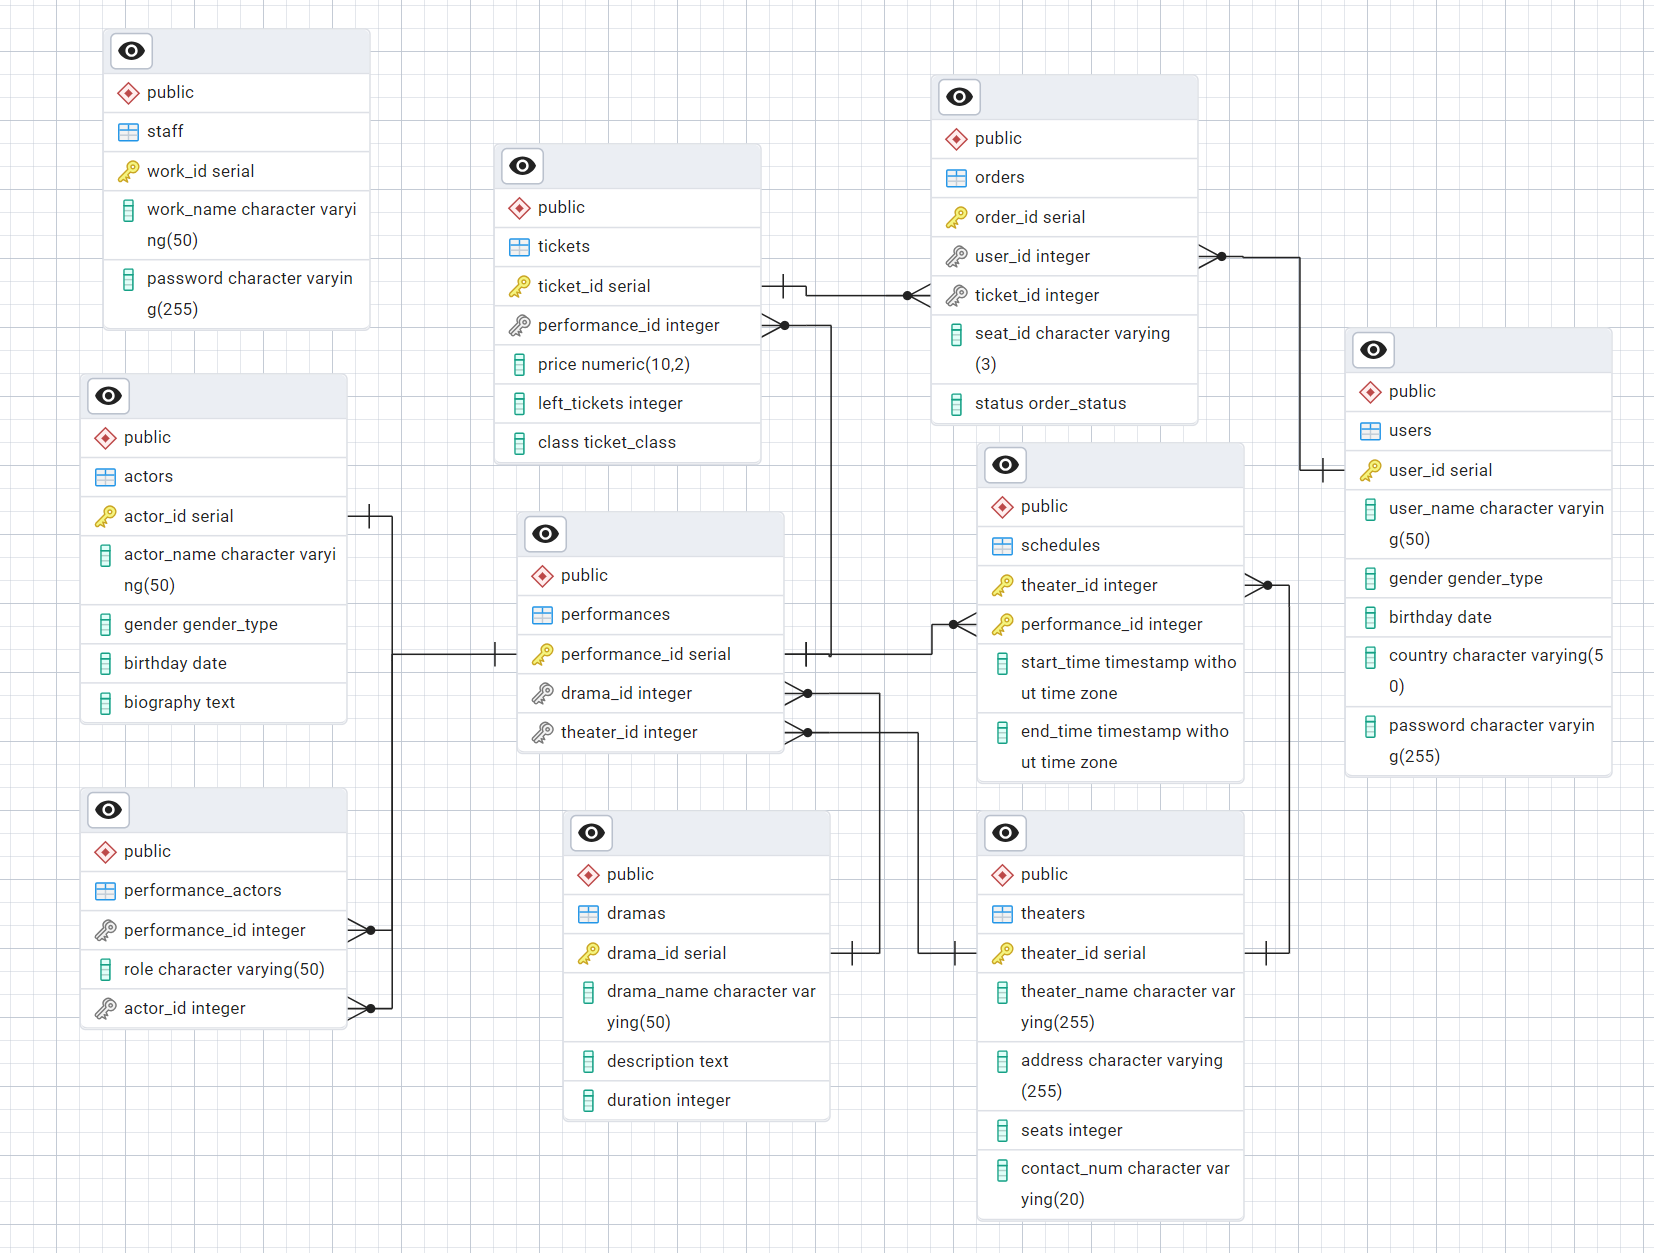
\includegraphics[width=\textwidth]{ER Model.png}
    \caption{ER Model}
    \label{Figure 1}
\end{figure}

\section{Function Design}
\par I have divided the program into two main functional modules: one for users and one for staff.
\par Users can log in and register, view all available information about dramas, actors, and theaters, and choose and purchase tickets based on personal preferences. They can also modify their personal information.
\par To ensure information security, staff can only log in and cannot register an account. Staff have the authority to modify, add, or delete drama information, actor information, theater information, and performance-related details.
\par The specific functional flowchart is shown in the figure below. I will omit the UI description and provide a detailed analysis of the database application part of the program.
\begin{figure}[h]
    \centering
    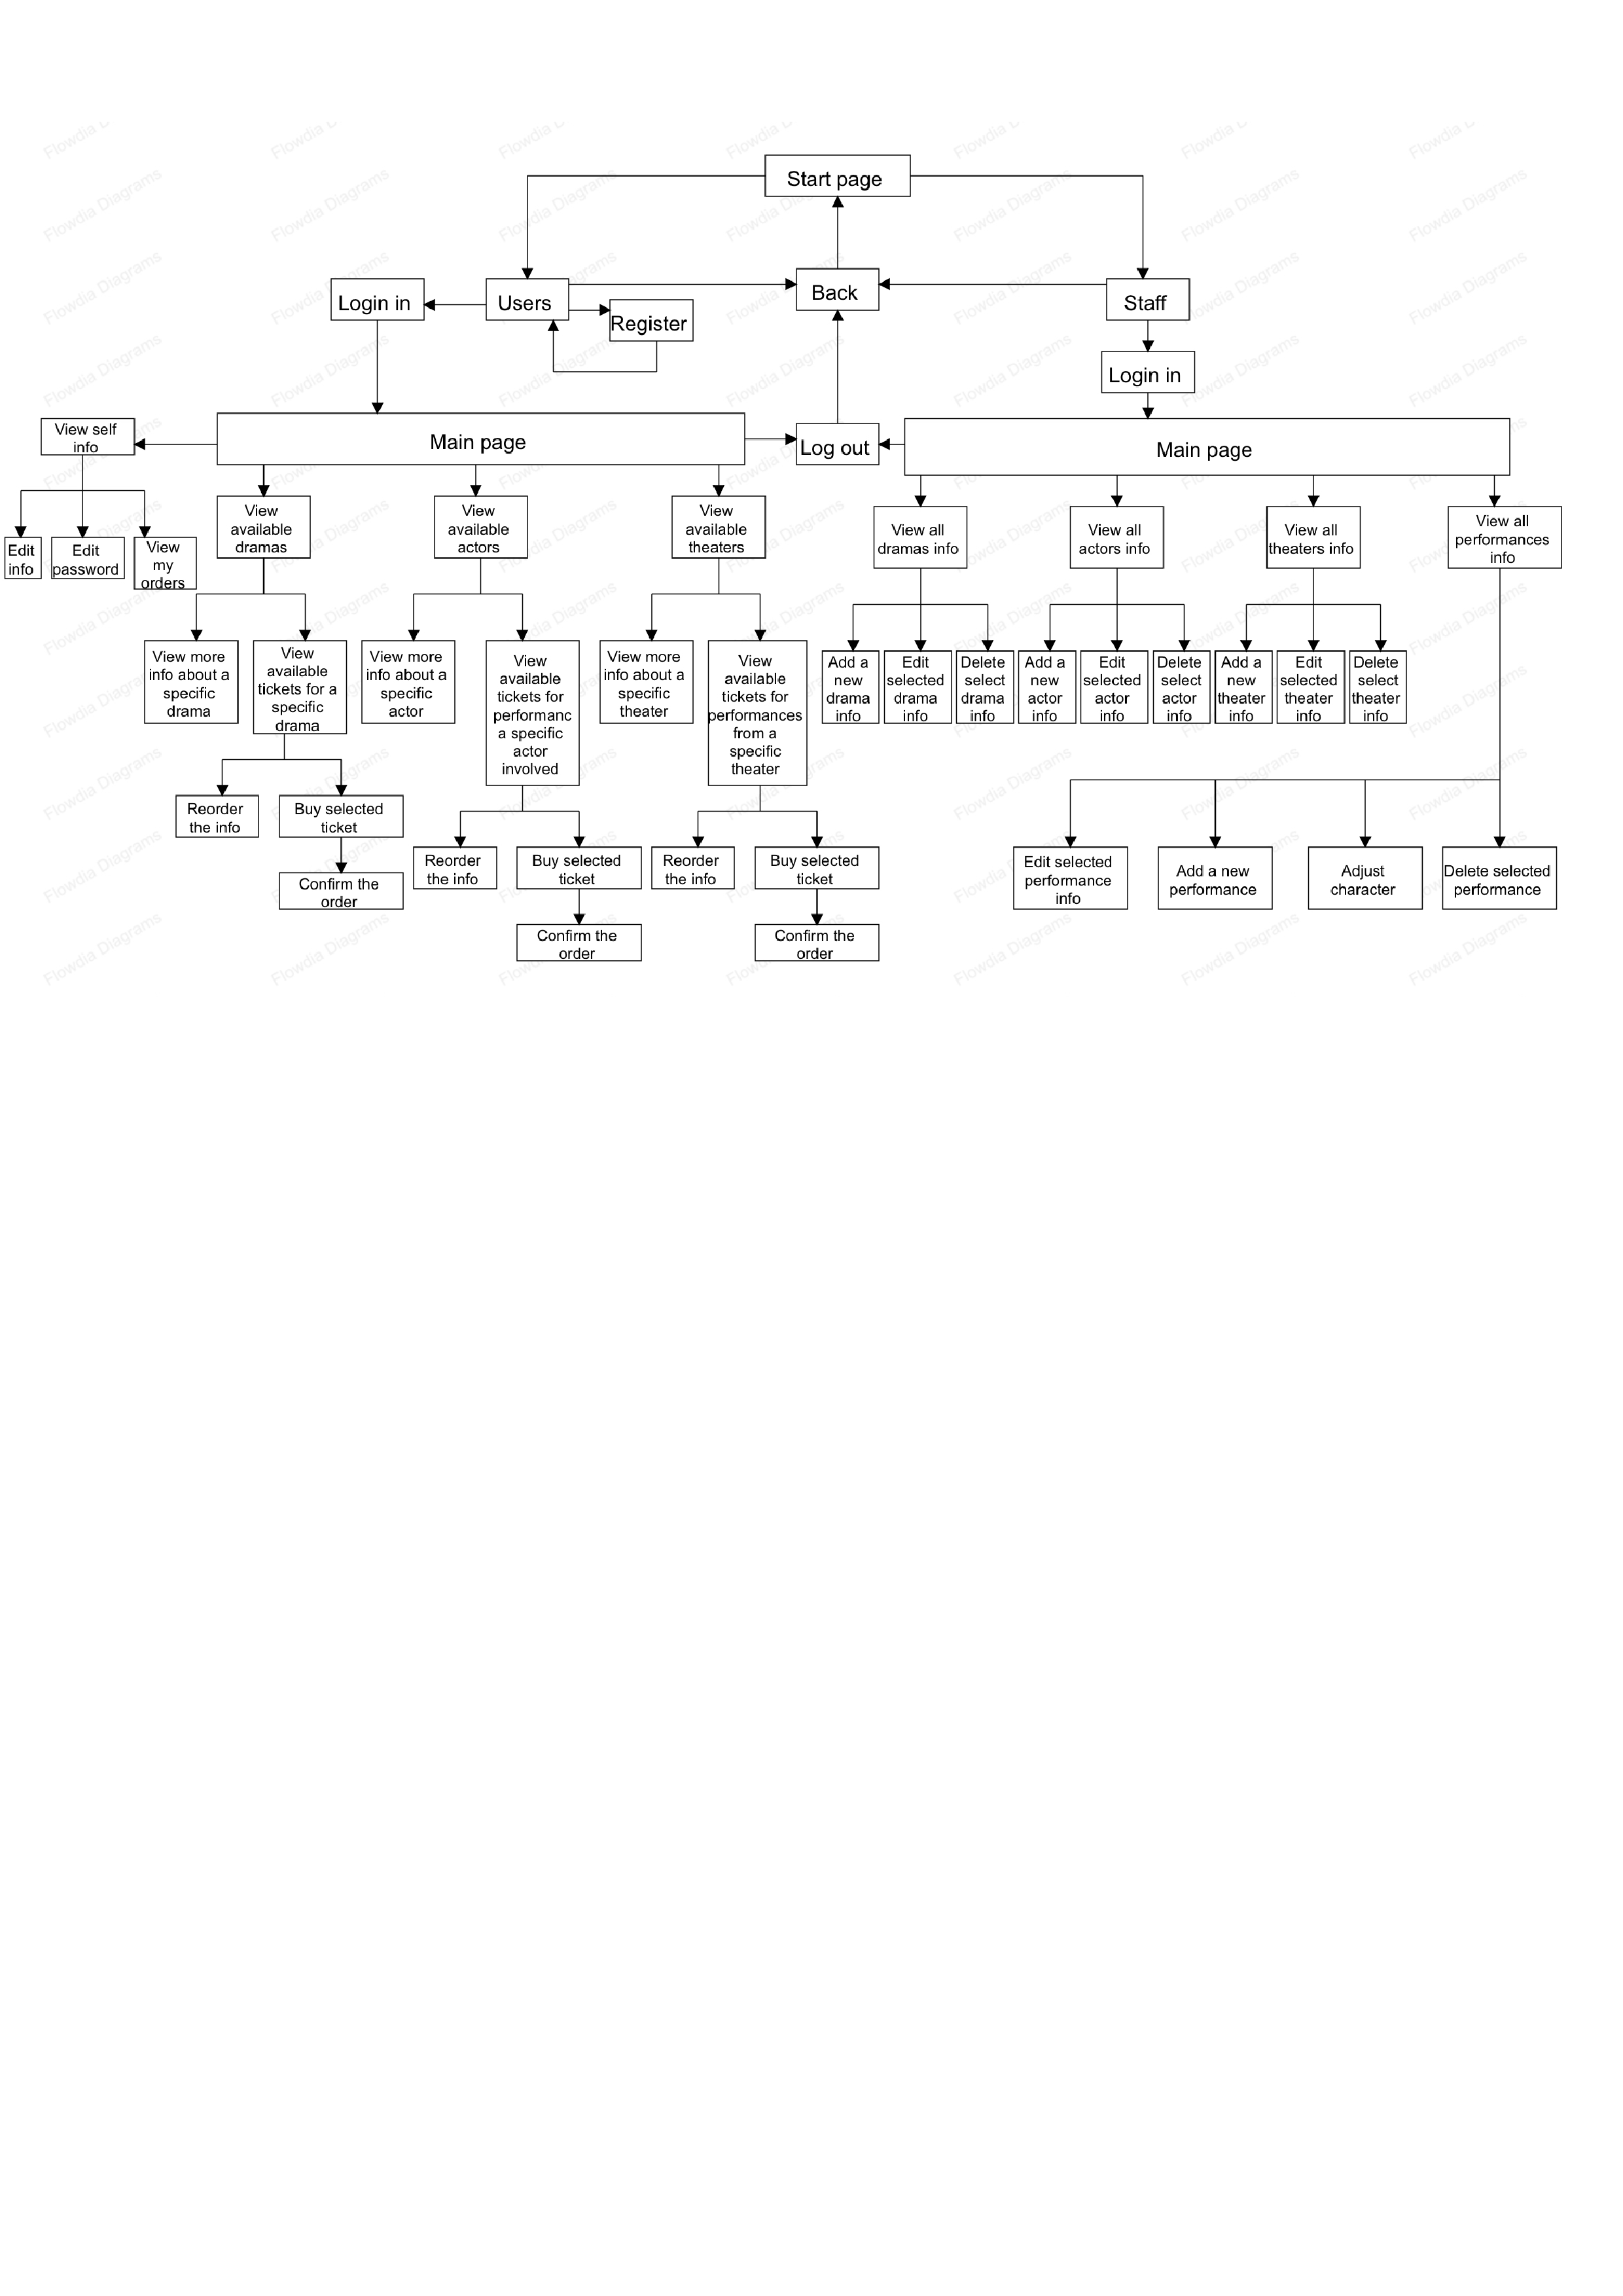
\includegraphics[width=0.95\textwidth]{Figure2.pdf}
    \caption{Functional flowchart}
    \label{Figure 2}
\end{figure}
\subsection{Users Function}
\subsubsection{Login Process Query}
\par During the login and registration process, the \textbf{users} table will be utilized. 
\par Since the \textbf{user\_id} is set as an auto-incrementing field when the table is created, users only need to input information other than the \textbf{user\_id}. After performing basic checks on this information, such as verifying whether all required fields are filled, ensuring the format is correct, and checking if the username already exists, the information will be written to the database using an \textbf{INSERT} statement.

\begin{tcolorbox}[colframe=black, colback=white, boxrule=0.4mm, sharp corners=southwest, title=Excerpt of User Registration Code]
    \begin{lstlisting}[language=Python, breaklines=true]
existing_user = db.fetch_one("""SELECT user_name 
    FROM users WHERE user_name = %s""", (user_name,))
if existing_user:
    show_error_message("""Username already exists""")
else:
    db.execute_query(""" 
        INSERT INTO users 
        (password, user_name, gender, birthday, country)
        VALUES (%s, %s, %s, %s, %s) 
        RETURNING user_id""",
        (password, user_name, gender, birthdate, country))
    user_id=db.fetch_one("""SELECT LASTVAL();""")[0]
    show_success_message(f"""Registration successful! Your User ID is {user_id}. \nPlease remember your ID for the next login.""")
\end{lstlisting}
\end{tcolorbox}

\par During login, the system first uses a \textbf{SELECT} statement to retrieve all user information. It first checks whether the \textbf{user\_id} entered by the user exists in the users table. If it does, the system then compares the entered password with the \textbf{password} corresponding to that \textbf{user\_id} in the database.

\begin{tcolorbox}[colframe=black, colback=white, boxrule=0.4mm, sharp corners=southwest, title=Excerpt of User Login Code]
    \begin{lstlisting}[language=Python, breaklines=true]
user = db.fetch_one("""SELECT * FROM users WHERE user_id = %s""", (user_id,))
stored_password = user[5] 
if password == stored_password:
    success_label = ctk.CTkLabel(window, text="""{}, welcome!""".format(user[1]), font=("Arial", 20), text_color="green")
    success_label.pack(pady=10)
    window.after(800, lambda: user_dashboard(window,user_id, db, pics,pics1,pics2)) 
else:
    messagebox.showerror("""Login Error""", """Incorrect password!\nPlease try again!""")
\end{lstlisting}
\end{tcolorbox}

\subsubsection{Drama-Based Query}
\par During this process, the \textbf{dramas}, \textbf{performances}, \textbf{tickets}, \textbf{orders} tables will be utilized. 
\par First, use a \textbf{SELECT} statement to retrieve all the drama information from the database, and then display it to the user combining both images and text.
\begin{tcolorbox}[colframe=black, colback=white, boxrule=0.4mm, sharp corners=southwest, title=Excerpt of Search Dramas Code]
    \begin{lstlisting}[language=Python, breaklines=true]
dramas = db.fetch_all("""SELECT * FROM dramas""")
\end{lstlisting}
\end{tcolorbox}

\par When the user selects a particular drama, a \textbf{SELECT} statement is used to retrieve the ticket information related to that drama through the relationship between \textbf{tickets} and \textbf{performances}. Then, using the relationships between \textbf{performances} and \textbf{schedules}, as well as between \textbf{performances} and \textbf{theaters}, all the ticket information is comprehensively displayed to the user. Additionally, the information can be sorted and filtered based on the user's desired sorting order and region.
\begin{tcolorbox}[colframe=black, colback=white, boxrule=0.4mm, sharp corners=southwest, title=Excerpt of Search Tickets Code]
    \begin{lstlisting}[language=Python, breaklines=true]
region_condition = ""
if region:
    region_condition = f"""AND H.address LIKE %s"""
    region = f"%{region}%"  # Use SQL LIKE pattern
query = f"""
        SELECT T.ticket_id, H.theater_name, S.start_time, S.end_time, T.class, T.price, T.left_tickets
        FROM tickets AS T
        JOIN performances AS P ON P.performance_id = T.performance_id
        JOIN Theaters AS H ON P.theater_id = H.theater_id
        JOIN schedules AS S ON P.performance_id = S.performance_id
        WHERE P.drama_id = %s
        {region_condition}
        ORDER BY {sort_column_map.get(sort_column, 'H.theater_name')} {sort_order_sql}
        """
tickets = db.fetch_all(query, (drama_id, region) if region else (drama_id,))
\end{lstlisting}
\end{tcolorbox}

\par After the user selects the ticket type, a \textbf{SELECT} statement is first used to retrieve all the existing orders of the user to check whether the user has already purchased the ticket, in order to prevent duplicate purchases. Once the user confirms the ticket purchase, an \textbf{UPDATE} statement is used to update the remaining \textbf{tickets}, decreasing the ticket count by one. Then, an \textbf{INSERT} statement is used to add the new order information to \textbf{orders}.
\begin{tcolorbox}[colframe=black, colback=white, boxrule=0.4mm, sharp corners=southwest, title=Excerpt of Buy Ticket Code]
    \begin{lstlisting}[language=Python, breaklines=true]
db.execute_query(
    """UPDATE tickets
        SET left_tickets = left_tickets - 1
        WHERE ticket_id = %s""",
        (ticket_id,))
seat_id = generate_seat_id(ticket_class)
db.execute_query(
    """INSERT INTO orders(user_id, ticket_id, seat_id, status)
        VALUES (%s, %s, %s, 'paid')""",
        (user_id, ticket_id, seat_id))
messagebox.showinfo("Success", f"""Successfully purchased one ticket! \nYour seat ID is {seat_id}\nYou can check your order in the <My Orders> page.""")
\end{lstlisting}
\end{tcolorbox}

\subsubsection{Actor-Based Query}
\par During this process, the \textbf{actors}, \textbf{performances}, \textbf{tickets}, \textbf{orders} and \textbf{performance\_actors} tables will be utilized. 
\par When the user wants to query \textbf{actors}, a \textbf{SELECT} statement is used to retrieve all the actor information, which is then displayed through a combination of images and text.
\begin{tcolorbox}[colframe=black, colback=white, boxrule=0.4mm, sharp corners=southwest, title=Excerpt of Search Actors Code]
    \begin{lstlisting}[language=Python, breaklines=true]
actors= db.fetch_all("""SELECT * FROM actors""")
\end{lstlisting}
\end{tcolorbox}

\par When the user selects an actor, a \textbf{SELECT} statement retrieves all ticket information for the \textbf{performances} the actor has participated in, based on the relationships between \textbf{tickets}, \textbf{performances}, and \textbf{performance\_actors}. The ticket details are then displayed using the relationships between \textbf{performances}, \textbf{schedules}, and \textbf{theaters}. Additionally, the information can be sorted and filtered by the user's preferred order and region.
\begin{tcolorbox}[colframe=black, colback=white, boxrule=0.4mm, sharp corners=southwest, title=Excerpt of Search Tickets Code]
    \begin{lstlisting}[language=Python, breaklines=true]
region_condition = ""
if region:
    region_condition = f"""AND H.address LIKE %s"""
    region = f"%{region}%"  
query = f"""SELECT T.ticket_id, D.drama_name,PA.role,H.theater_name, S.start_time, S.end_time, T.class, T.price, T.left_tickets
    FROM tickets AS T
    JOIN performances AS P ON P.performance_id = T.performance_id
    JOIN theaters AS H ON P.theater_id = H.theater_id
    JOIN schedules AS S ON P.performance_id = S.performance_id
    JOIN dramas AS D ON D.drama_id = P.drama_id
    JOIN performance_actors AS PA ON PA.performance_id = P.performance_id
    JOIN actors AS A ON A.actor_id = PA.actor_id
    WHERE A.actor_id = %s {region_condition}
    ORDER BY {sort_column_map.get(sort_column, 'H.theater_name')} {sort_order_sql}"""
tickets = db.fetch_all(query, (actor_id, region) if region else (actor_id,))
\end{lstlisting}
\end{tcolorbox}
\par The database used for subsequent ticket purchases is the same as the one described earlier, so it is omitted.

\subsubsection{Theater-Based Query}
\par During this process, the \textbf{theaters}, \textbf{performances}, \textbf{tickets}, \textbf{orders} tables will be utilized. 
\par When the user wants to query \textbf{theaters}, a \textbf{SELECT} statement is used to retrieve all the theater information, which is then displayed through a combination of images and text.
\begin{tcolorbox}[colframe=black, colback=white, boxrule=0.4mm, sharp corners=southwest, title=Excerpt of Search Theaters Code]
    \begin{lstlisting}[language=Python, breaklines=true]
theaters=db.fetch_all("""SELECT * FROM theaters""")
\end{lstlisting}
\end{tcolorbox}

\par When the user selects a theater, a \textbf{SELECT} statement retrieves all ticket information for performances at that theater, based on the relationships between \textbf{theaters}, \textbf{performances}, and \textbf{tickets}. The details are displayed using the relationships with \textbf{dramas} and \textbf{schedules}. The information can be sorted and filtered by the user's preferences. Unlike previous sorting processes, the \textbf{LIKE} statement is not used for region filtering, as the theater already defines the location.
\begin{tcolorbox}[colframe=black, colback=white, boxrule=0.4mm, sharp corners=southwest, title=Excerpt of Search Tickets Code]
    \begin{lstlisting}[language=Python, breaklines=true]
query = f"""SELECT T.ticket_id, D.drama_name, H.theater_name, S.start_time, S.end_time, T.class, T.price, T.left_tickets
    FROM tickets AS T
    JOIN performances AS P ON P.performance_id = T.performance_id
    JOIN theaters AS H ON P.theater_id = H.theater_id
    JOIN schedules AS S ON P.performance_id = S.performance_id
    JOIN dramas AS D ON D.drama_id = P.drama_id
    WHERE H.theater_id = %s
    ORDER BY {sort_column_map.get(sort_column, 'H.theater_name')} {sort_order_sql}
tickets = db.fetch_all(query, (theater_id,))
\end{lstlisting}
\end{tcolorbox}

\par The database used for subsequent ticket purchases is the same as the one described earlier, so it is omitted.

\subsubsection{Personal Information Query}
\par When the user views his or her information, the corresponding data is retrieved from the \textbf{users} table based on the \textbf{user\_id} and displayed. 
\begin{tcolorbox}[colframe=black, colback=white, boxrule=0.4mm, sharp corners=southwest, title=Excerpt of Search Personal Info Code]
    \begin{lstlisting}[language=Python, breaklines=true]
user_info = db.fetch_one("""SELECT * FROM users WHERE user_id=%s""", (user_id,))
\end{lstlisting}
\end{tcolorbox}

\par When the user edits their personal information, the submitted content is briefly reviewed, and the \textbf{users} is updated using an \textbf{UPDATE} statement. 
\begin{tcolorbox}[colframe=black, colback=white, boxrule=0.4mm, sharp corners=southwest, title=Excerpt of Edit Personal Info Code]
    \begin{lstlisting}[language=Python, breaklines=true]
db.excute_query("""UPDATE users SET user_name=%s, gender=%s, birthday=%s, country=%s WHERE user_id=%s""", 
    (new_name, new_gender, new_birthdate, new_country, user_id))
\end{lstlisting}
\end{tcolorbox}

\par When the user changes their password, both the new and old passwords must be provided. A \textbf{SELECT} statement retrieves the current password for comparison to ensure account security.
\begin{tcolorbox}[colframe=black, colback=white, boxrule=0.4mm, sharp corners=southwest, title=Excerpt of Edit Password Code]
    \begin{lstlisting}[language=Python, breaklines=true]
if old_password != current_password:
    messagebox.showerror("Error","""Old password is incorrect! Please try again.""")
elif not new_password: 
    messagebox.showerror("Error", """New password cannot be empty! Please try again.""")
else: 
    db.execute_query("""UPDATE users 
    SET password=%s WHERE user_id=%s""", (new_password, user_id))
    messagebox.showinfo("Success", """Password changed successfully!""")
\end{lstlisting}
\end{tcolorbox}

\par When the user queries all their orders, a \textbf{SELECT} statement is used to query the corresponding orders in the \textbf{orders} table. Then, based on the relationships with \textbf{performances}, \textbf{theaters}, \textbf{dramas}, and \textbf{schedules}, the complete order details are output, providing the user with the most comprehensive information.
\begin{tcolorbox}[colframe=black, colback=white, boxrule=0.4mm, sharp corners=southwest, title=Excerpt of Search Personal Orders Code]
    \begin{lstlisting}[language=Python, breaklines=true]
query = """
    SELECT orders.order_id, orders.seat_id, 
    tickets.price, dramas.drama_name, 
    dramas.duration, schedules.start_time, 
    schedules.end_time, theaters.theater_name, 
    theaters.address  
    FROM orders
    RIGHT JOIN tickets ON tickets.ticket_id = orders.ticket_id
    RIGHT JOIN performances ON performances.performance_id = tickets.performance_id
    RIGHT JOIN dramas ON dramas.drama_id = performances.drama_id
    RIGHT JOIN schedules ON schedules.performance_id = performances.performance_id
    RIGHT JOIN theaters ON theaters.theater_id = performances.theater_id
    WHERE orders.user_id = %s"""
orders = db.fetch_all(query, (user_id,))
\end{lstlisting}
\end{tcolorbox}

\subsection{Staff Function}
\subsubsection{Login Process Query}
\par During the login process, the \textbf{staff} table will be utilized. 
Staff can only log in, and the process is the same as the user login process.

\begin{tcolorbox}[colframe=black, colback=white, boxrule=0.4mm, sharp corners=southwest, title=Excerpt of Staff Login Code]
    \begin{lstlisting}[language=Python, breaklines=true]
staff = db.fetch_one("""SELECT * FROM staff WHERE work_id = %s""", (work_id,))
if staff is None:
    messagebox.showerror("Error", """Invalid Work ID!""")
else:
    stored_password = staff[2]
    if password == stored_password:
        success_label = ctk.CTkLabel(window, text="""{}, welcome!""".format(staff[1]), font=("Arial", 20), text_color="green")
        success_label.pack(pady=10)
        window.after(800, lambda: staff_dashboard(window,work_id, db))
    else:
        messagebox.showerror("Error", """Incorrect password!\nPlease try again!""")
\end{lstlisting}
\end{tcolorbox}

\subsubsection{Drama Management Query} 
\par The \textbf{dramas} table is used to manage the drama information.
\par When the staff selects the drama section, all the information from the \textbf{dramas} table needs to be displayed. 
\par When a new drama is to be added, the staff's input is briefly reviewed, and the information is inserted into the dramas table using an \textbf{INSERT} statement. 
\begin{tcolorbox}[colframe=black, colback=white, boxrule=0.4mm, sharp corners=southwest, title=Excerpt of Drama Add Code]
    \begin{lstlisting}[language=Python, breaklines=true]
query = """INSERT INTO dramas (drama_name, description, duration) VALUES (%s, %s, %s)"""
db.execute_query(query, (name_entry, description_entry, duration_entry))
\end{lstlisting}
\end{tcolorbox}

\par When the user needs to delete the selected drama, the related foreign key data is deleted first, and then the corresponding information is removed from the \textbf{dramas} table using a \textbf{DELETE} statement.
\begin{tcolorbox}[colframe=black, colback=white, boxrule=0.4mm, sharp corners=southwest, title=Excerpt of Drama Deletion Code]
    \begin{lstlisting}[language=Python, breaklines=true]
drama_id = treeview.item(selected_item[0])['values'][0]
performance_ids = db.fetch_all("""SELECT performance_id FROM performances WHERE drama_id = %s""", (drama_id,))
query3 = """DELETE FROM tickets WHERE performance_id = %s"""
query4 = """DELETE FROM performance_actors WHERE performance_id = %s"""
query5 = """DELETE FROM schedules WHERE performance_id = %s"""
query1 = """DELETE FROM performances WHERE drama_id = %s"""
query2 = """DELETE FROM dramas WHERE drama_id = %s"""
for performance in performance_ids:
    performance_id = performance
    db.execute_query(query5, (performance_id,))
    db.execute_query(query4, (performance_id,))
    db.execute_query(query3, (performance_id,))
db.execute_query(query1, (drama_id,))
db.execute_query(query2, (drama_id,))
\end{lstlisting}
\end{tcolorbox}

\par When the user needs to modify the selected drama, the staff's input is reviewed, and the changes are applied to the \textbf{dramas} table using an \textbf{UPDATE} statement.
\begin{tcolorbox}[colframe=black, colback=white, boxrule=0.4mm, sharp corners=southwest, title=Excerpt of Drama Edit Code]
    \begin{lstlisting}[language=Python, breaklines=true]
query = """UPDATE dramas SET drama_name = %s, description = %s, duration = %s WHERE drama_id = %s"""
db.execute_query(query, (drama_name, description, duration, drama_id))
\end{lstlisting}
\end{tcolorbox}

\subsubsection{Actor Management Query}
\par The \textbf{actors} table is used to manage the actor information.
\par When the staff selects the actor section, all the information from the \textbf{actors} table needs to be displayed.
\par When a new actor's information is to be added, the staff's input is briefly reviewed, and the information is inserted into the \textbf{actors} table using an \textbf{INSERT} statement.
\begin{tcolorbox}[colframe=black, colback=white, boxrule=0.4mm, sharp corners=southwest, title=Excerpt of Actor Add Code]
    \begin{lstlisting}[language=Python, breaklines=true]
query = """INSERT INTO actors (actor_name, biography, gender,birthday) VALUES (%s, %s, %s,%s)"""
db.execute_query(query, (name_entry, description_entry, gender_entry,birthdate_entry))
\end{lstlisting}
\end{tcolorbox}

\par When the staff needs to delete a selected actor, the related foreign key data is deleted first using a \textbf{DELETE} statement, followed by the deletion of the actor's information from the \textbf{actors} table.
\begin{tcolorbox}[colframe=black, colback=white, boxrule=0.4mm, sharp corners=southwest, title=Excerpt of Actor Deletion Code]
    \begin{lstlisting}[language=Python, breaklines=true]
actor_id = treeview.item(selected_item[0])['values'][0]  
query1 = """DELETE FROM performance_actors WHERE actor_id = %s"""
query2 = """DELETE FROM actors WHERE actor_id = %s"""
db.execute_query(query1, (actor_id,))
db.execute_query(query2, (actor_id,))
\end{lstlisting}
\end{tcolorbox}

\par When the actor's information needs to be modified, an \textbf{UPDATE} statement is used.
\begin{tcolorbox}[colframe=black, colback=white, boxrule=0.4mm, sharp corners=southwest, title=Excerpt of Actor Edit Code]
    \begin{lstlisting}[language=Python, breaklines=true]
query = """UPDATE actors SET actor_name = %s, gender = %s, birthday = %s, biography = %s WHERE actor_id = %s"""
db.execute_query(query, (actor_name, gender, birthdate, biography, actor_id))
\end{lstlisting}
\end{tcolorbox}

\subsubsection{Theater Management Query}
\par The \textbf{theaters} table is used to manage the theater information.
\par When the staff selects the theater section, all the information from the \textbf{theaters} table needs to be displayed.
\par When a new theater's information is to be added, the staff's input is briefly reviewed, and the information is inserted into the \textbf{theaters} table using an \textbf{INSERT} statement.
\begin{tcolorbox}[colframe=black, colback=white, boxrule=0.4mm, sharp corners=southwest, title=Excerpt of Theater Add Code]
    \begin{lstlisting}[language=Python, breaklines=true]
query = """INSERT INTO theaters (theater_name, address, seats, contact_num) VALUES (%s, %s, %s, %s)"""
db.execute_query(query, (name_entry, address_entry, seats_entry, contact_entry))
\end{lstlisting}
\end{tcolorbox}
\par When the staff needs to delete a selected theater, the related foreign key data is deleted first using a \textbf{DELETE} statement, followed by the deletion of the theater's information from the \textbf{theaters} table.
\begin{tcolorbox}[colframe=black, colback=white, boxrule=0.4mm, sharp corners=southwest, title=Excerpt of Theater Deletion Code]
    \begin{lstlisting}[language=Python, breaklines=true]
theater_id = treeview.item(selected_item[0])['values'][0]
performance_ids = db.fetch_all("""SELECT performance_id FROM performances WHERE theater_id = %s""", (theater_id,))
query_schedule = """DELETE FROM schedules WHERE theater_id = %s"""
query_ticket = """DELETE FROM tickets WHERE performance_id = %s"""
query_performance_actors = """DELETE FROM performance_actors WHERE performance_id = %s"""
query_performance ="""DELETE FROM performances WHERE performance_id = %s"""
query_theater = """DELETE FROM theaters WHERE theater_id = %s"""
db.execute_query(query_schedule, (theater_id,))
for performance in performance_ids:
    performance_id = performance[0]
    db.execute_query(query_ticket, (performance_id,))
    db.execute_query(query_performance_actors, (performance_id,))
    db.execute_query(query_performance, (performance_id,))
db.execute_query(query_theater, (theater_id,))
\end{lstlisting}
\end{tcolorbox}

\par When the theater's information needs to be modified, an \textbf{UPDATE} statement is used.
\begin{tcolorbox}[colframe=black, colback=white, boxrule=0.4mm, sharp corners=southwest, title=Excerpt of Theater Edit Code]
    \begin{lstlisting}[language=Python, breaklines=true]
query = """UPDATE theaters SET theater_name = %s, address = %s, seats = %s, contact_num = %s WHERE theater_id = %s"""
db.execute_query(query, (theater_name, address, seats, contact, theater_id))
\end{lstlisting}
\end{tcolorbox}

\subsubsection{Performance Management Query}
\par This process involves the \textbf{performances}, \textbf{actors}, \textbf{performance\_actors}, \textbf{theaters}, \textbf{dramas}, and \textbf{schedules} tables, as a performance's information includes a combination of details such as the drama, performance time, and venue.
\par When displaying all performance information, the data from multiple tables is first combined using the \textbf{performance\_id} to generate the performance details, and then the \textbf{performance\_actors} table is used to link the information to the actors.
\begin{tcolorbox}[colframe=black, colback=white, boxrule=0.4mm, sharp corners=southwest, title=Excerpt of Performance show Code]
    \begin{lstlisting}[language=Python, breaklines=true]
performances = db.fetch_all("""
    SELECT 
    performances.performance_id, dramas.drama_name, 
    theaters.theater_name, actors.actor_name, 
    performance_actors.role, schedules.start_time,
    schedules.end_time
    FROM performances 
    LEFT JOIN theaters ON performances.theater_id = theaters.theater_id 
    LEFT JOIN dramas ON dramas.drama_id = performances.drama_id
    LEFT JOIN performance_actors ON performance_actors.performance_id = performances.performance_id
    LEFT JOIN actors ON actors.actor_id = performance_actors.actor_id
    LEFT JOIN schedules ON performances.performance_id = schedules.performance_id;""")
\end{lstlisting}
\end{tcolorbox}
\par When modifying selected performance details, such as the drama name, venue, and time, the staff only needs to provide the updated information. The primary key of the new data is then found in the corresponding table and updated in the \textbf{performances} table, followed by updating the corresponding time for that performance\_id in the \textbf{schedules} table.
\begin{tcolorbox}[colframe=black, colback=white, boxrule=0.4mm, sharp corners=southwest, title=Excerpt of Performance Edit Code]
    \begin{lstlisting}[language=Python, breaklines=true]
performance_info = treeview.item(selected_item[0])['values']
performance_id, drama_name, theater_name, actor, role, start_time, end_time = performance_info
theater_id = db.fetch_one("""SELECT theater_id FROM theaters WHERE theater_name=%s""", (updated_theater_name,))[0]
drama_id = db.fetch_one("""SELECT drama_id FROM dramas WHERE drama_name=%s""", (updated_drama_name,))[0]
query_performance = """
    UPDATE performances, schedules
    JOIN theaters ON performances.theater_id = theaters.theater_id
    JOIN schedules ON schedules.performance_id = performances.performance_id
    SET performances.theater_id = %s,
        performances.drama_id = %s,
        schedules.start_time = %s,
        schedules.end_time = %s
    WHERE performances.performance_id = %s"""
db.execute_query(query_performance, (theater_id, drama_id, updated_start_time, updated_end_time, performance_id))
\end{lstlisting}
\end{tcolorbox}

\par When adding a performance, the staff needs to provide all relevant performance information, but does not need to include actor role information. Then, the corresponding primary key is found and the data is added to the \textbf{performances} table using an \textbf{INSERT} statement.
\begin{tcolorbox}[colframe=black, colback=white, boxrule=0.4mm, sharp corners=southwest, title=Excerpt of Performance Add Code]
    \begin{lstlisting}[language=Python, breaklines=true]
drama_id = db.fetch_one("""SELECT drama_id FROM dramas WHERE drama_name=%s""", (drama_name,))[0]
theater_id = db.fetch_one("""SELECT theater_id FROM theaters WHERE theater_name=%s""",(theater_name))[0]
query = """
    INSERT INTO performances (drama_id, theater_id)
    VALUES (%s, %s)"""
db.execute_query(query, (drama_id, theater_id,))
\end{lstlisting}
\end{tcolorbox}

\par When the staff wants to adjust the role information for a performance, they need to input the performance\_id, actor name, and role name, and then update or add the corresponding data to the \textbf{performance\_actors} table.
\begin{tcolorbox}[colframe=black, colback=white, boxrule=0.4mm, sharp corners=southwest, title=Excerpt of Charator Adjust Code]
    \begin{lstlisting}[language=Python, breaklines=true]
if role in existing_roles:
    confirm = messagebox.askyesno("Confirm", """The role exists.\nDo you want to replace it?""")
    if confirm:
        db.execute_query("""UPDATE performance_actors
            SET actor_id = (SELECT actor_id FROM actors WHERE actor_name = %s)
            WHERE performance_id = %s AND role = %s
            """, (actor_name, performance_id, role))
else:
    actor_id = db.fetch_one("""SELECT actor_id FROM actors WHERE actor_name = %s""", (actor_name,))
    if actor_id is None:
        messagebox.showerror("Error", """Actor not found in the database!""")
        return
    actor_id = actor_id[0]
    db.execute_query("""
        INSERT INTO performance_actors (performance_id, role, actor_id)
         VALUES (%s, %s, %s)
        """, (performance_id, role, actor_id))
\end{lstlisting}
\end{tcolorbox}

\par When deleting a performance, all related foreign key information must be deleted first, followed by the deletion of the performance itself.
\begin{tcolorbox}[colframe=black, colback=white, boxrule=0.4mm, sharp corners=southwest, title=Excerpt of Performance Delete Code]
    \begin{lstlisting}[language=Python, breaklines=true]
erformance_id = treeview.item(selected_item[0])['values'][0]
query1 = """DELETE FROM performances WHERE performance_id = %s"""
query2 = """DELETE FROM tickets WHERE performance_id = %s"""
query3 = """DELETE FROM schedules WHERE performance_id = %s"""
query4 = """DELETE FROM performance_actors WHERE performance_id = %s"""
db.execute_query(query4, (performance_id,))
db.execute_query(query3, (performance_id,))
db.execute_query(query2, (performance_id,))
db.execute_query(query1, (performance_id,))
\end{lstlisting}
\end{tcolorbox}

\section{Implementation}

\begin{figure}[H]
    \centering
    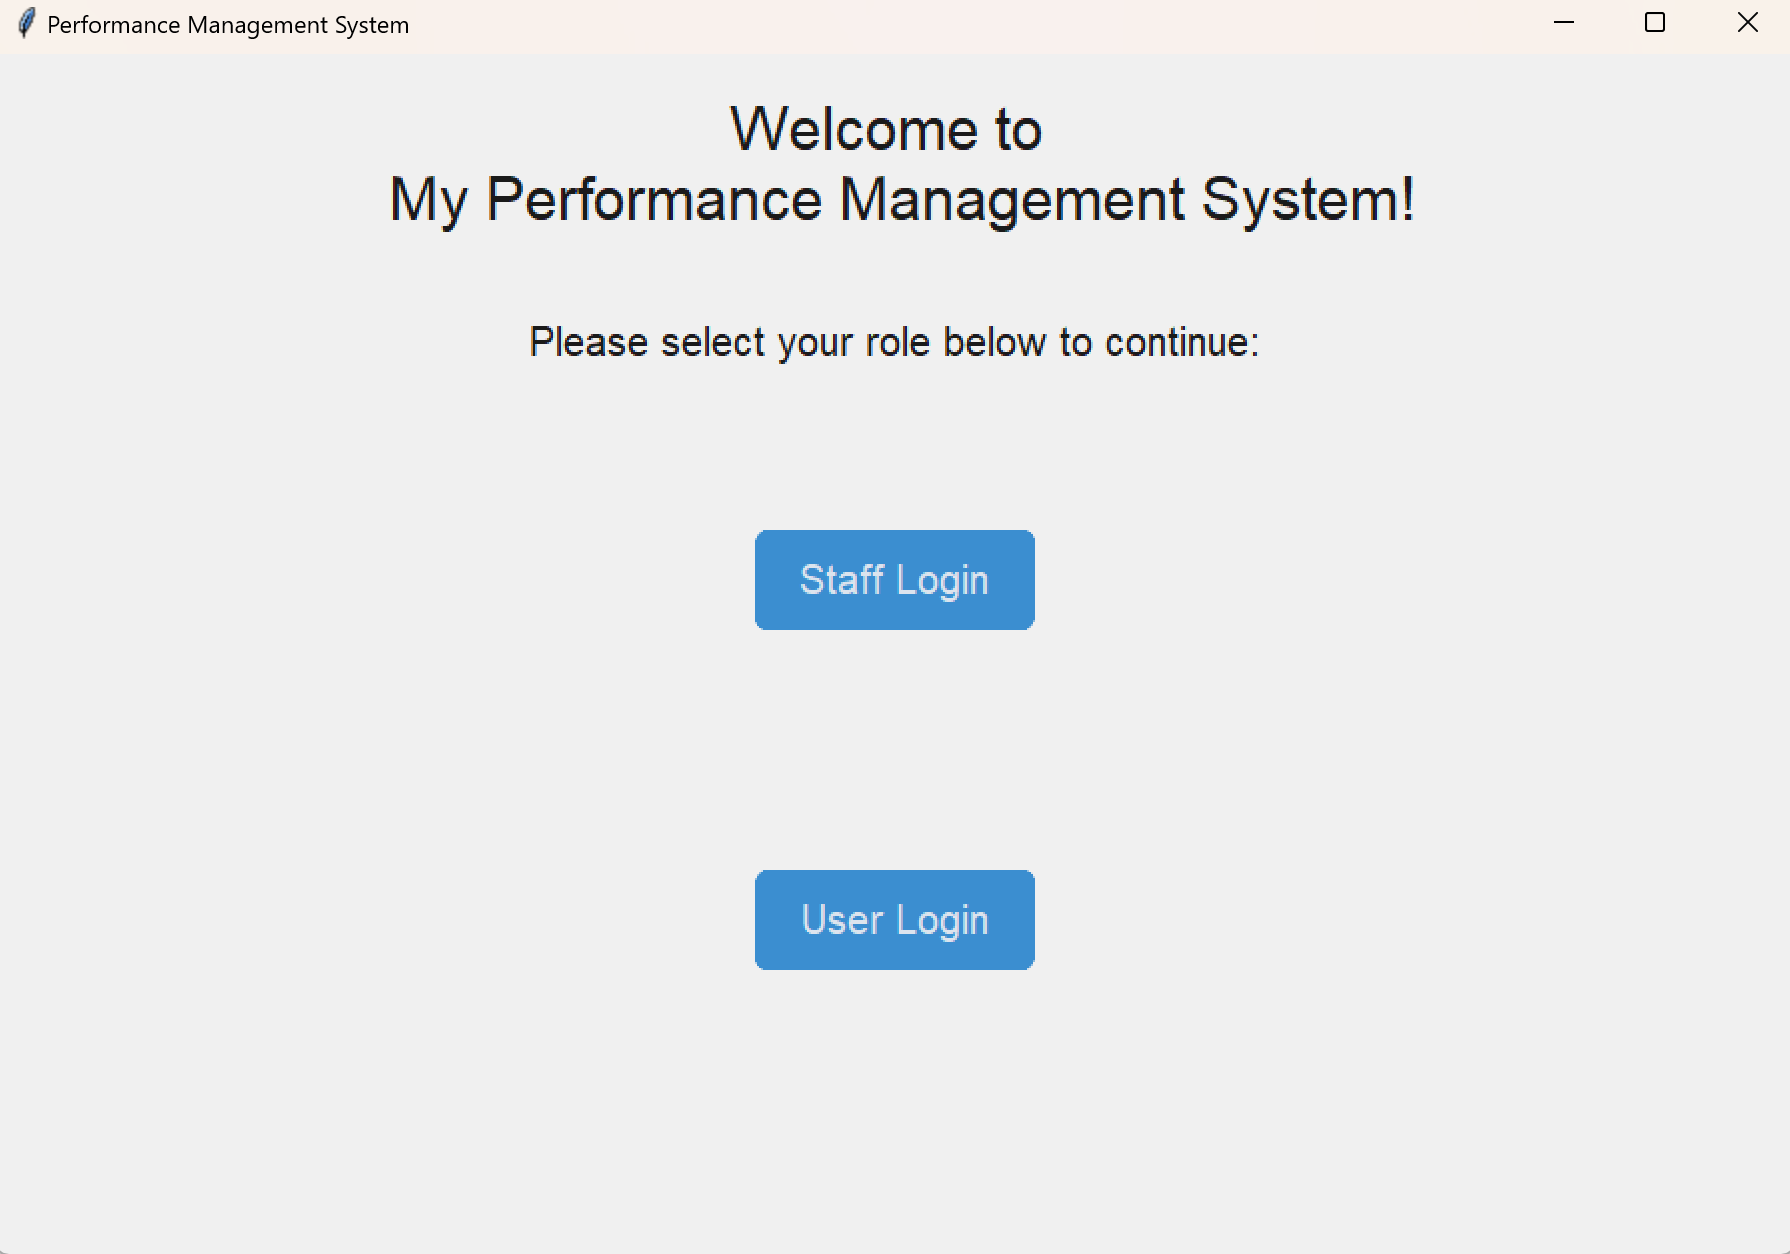
\includegraphics[width=0.75\textwidth]{3.png}
    \caption{Initial interface}
    \label{Figure 3}
\end{figure}

\subsection{User Usage}
\par Users can log in using their username and password. Upon successful login, the username will be displayed to welcome the user. If the login fails, an error message will pop up, prompting the user to re-enter the information. Users without an account can click on 'Register' and fill in the information in the registration popup to sign up.
Users can also click the 'Back' button in the top left corner to return and select a different role.
\begin{figure}[H]
    \centering
    \begin{minipage}{0.58\textwidth}
        \centering
        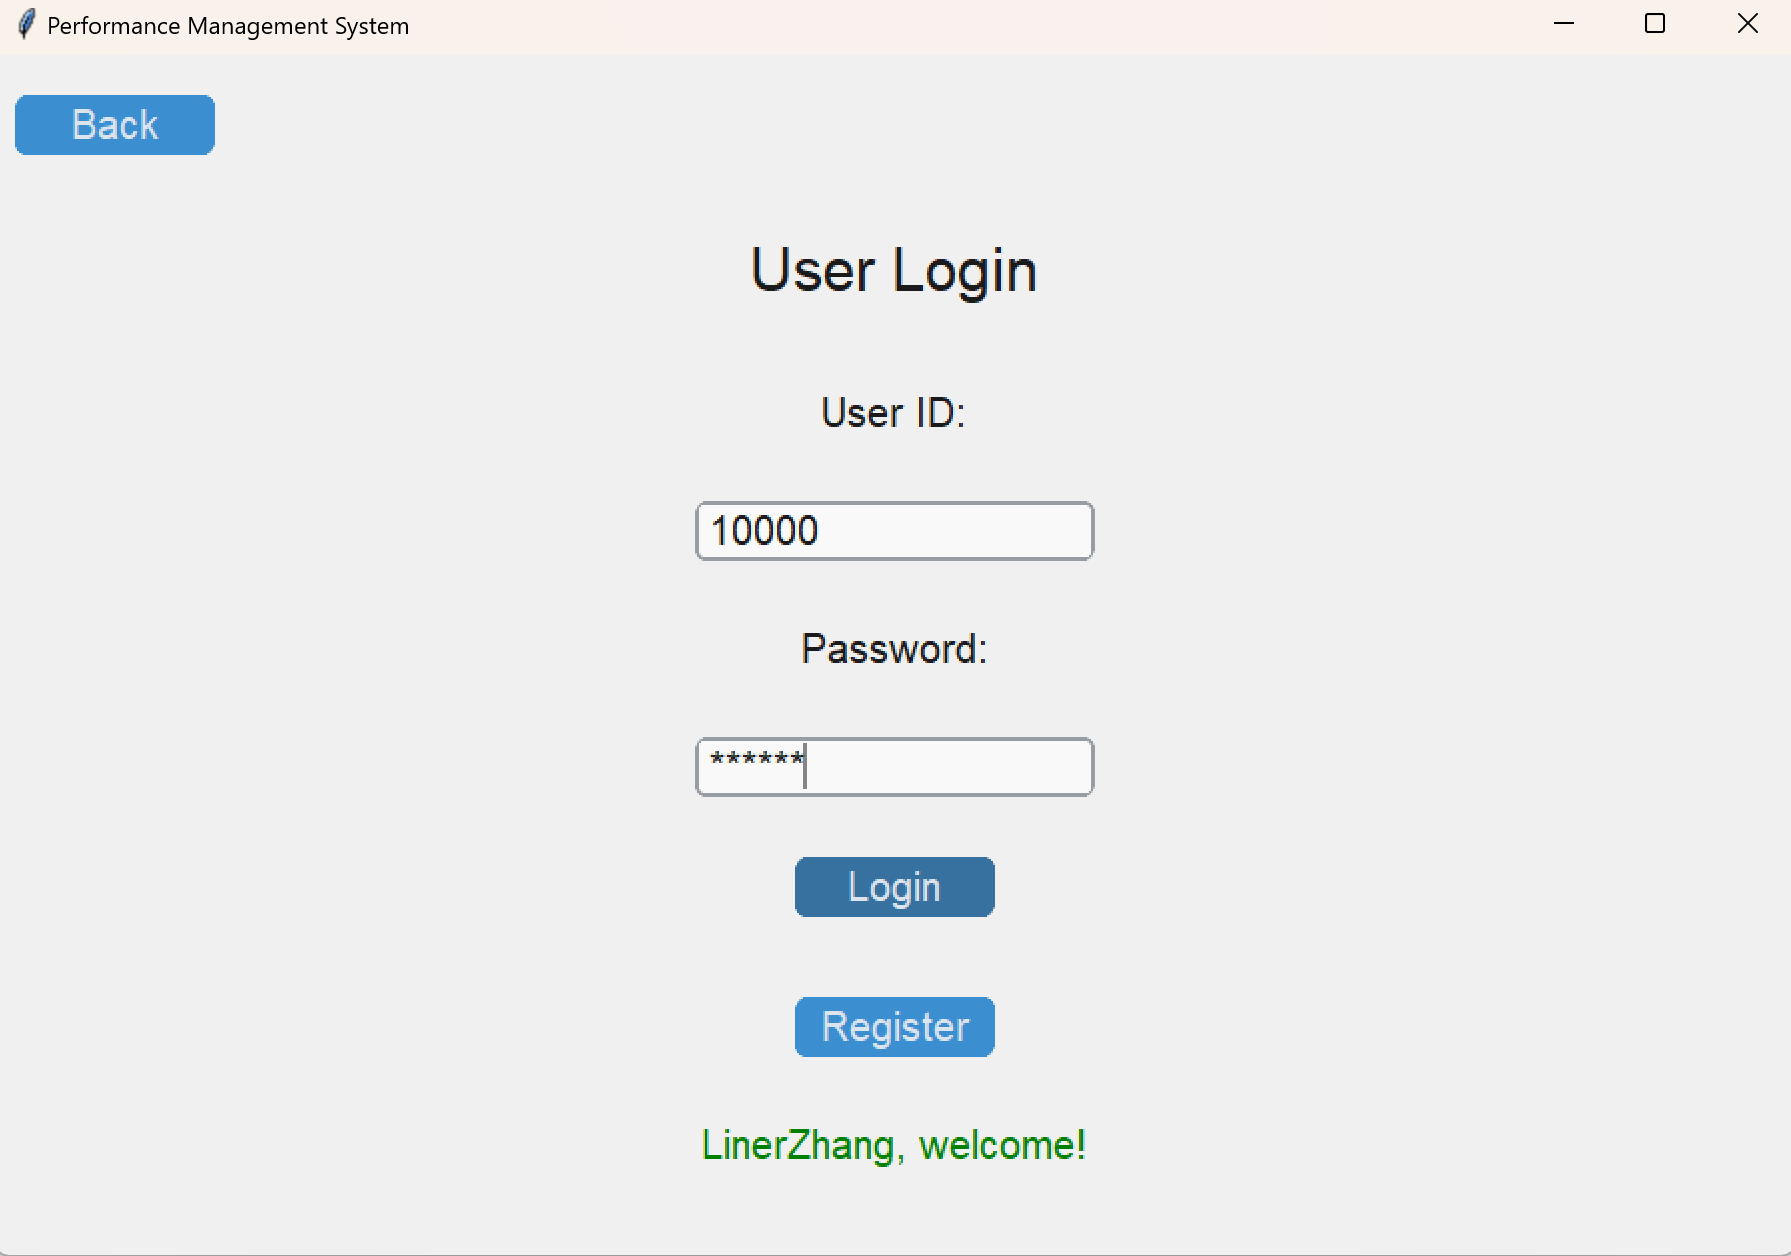
\includegraphics[width=\textwidth]{4.png}
        \caption{User login}
        \label{Figure 4}
    \end{minipage}
    \hfill
    \begin{minipage}{0.35\textwidth}
        \centering
        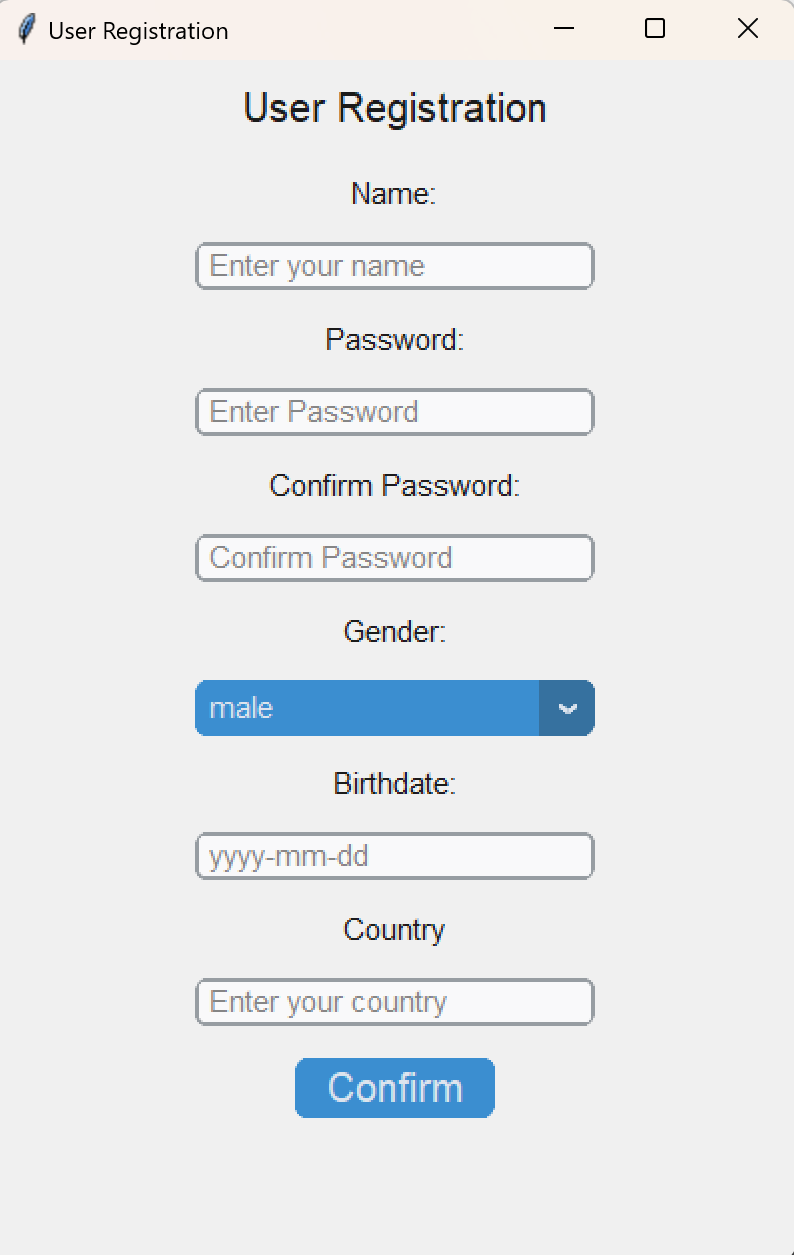
\includegraphics[width=\textwidth]{5.png}
        \caption{User registration}
        \label{Figure 5}
    \end{minipage}
\end{figure}

\par After logging in, the interface is divided into three main sections. The top row contains two buttons: the left button allows the user to log out and return to the initial screen, while the right button allows the user to view and manage their personal information. The left section contains three buttons for querying and displaying different types of information. The right section is the display area, which by default shows drama information, with two items per page and the ability to paginate.

\begin{figure}[H]
    \centering
    \begin{minipage}{0.48\textwidth}
        \centering
        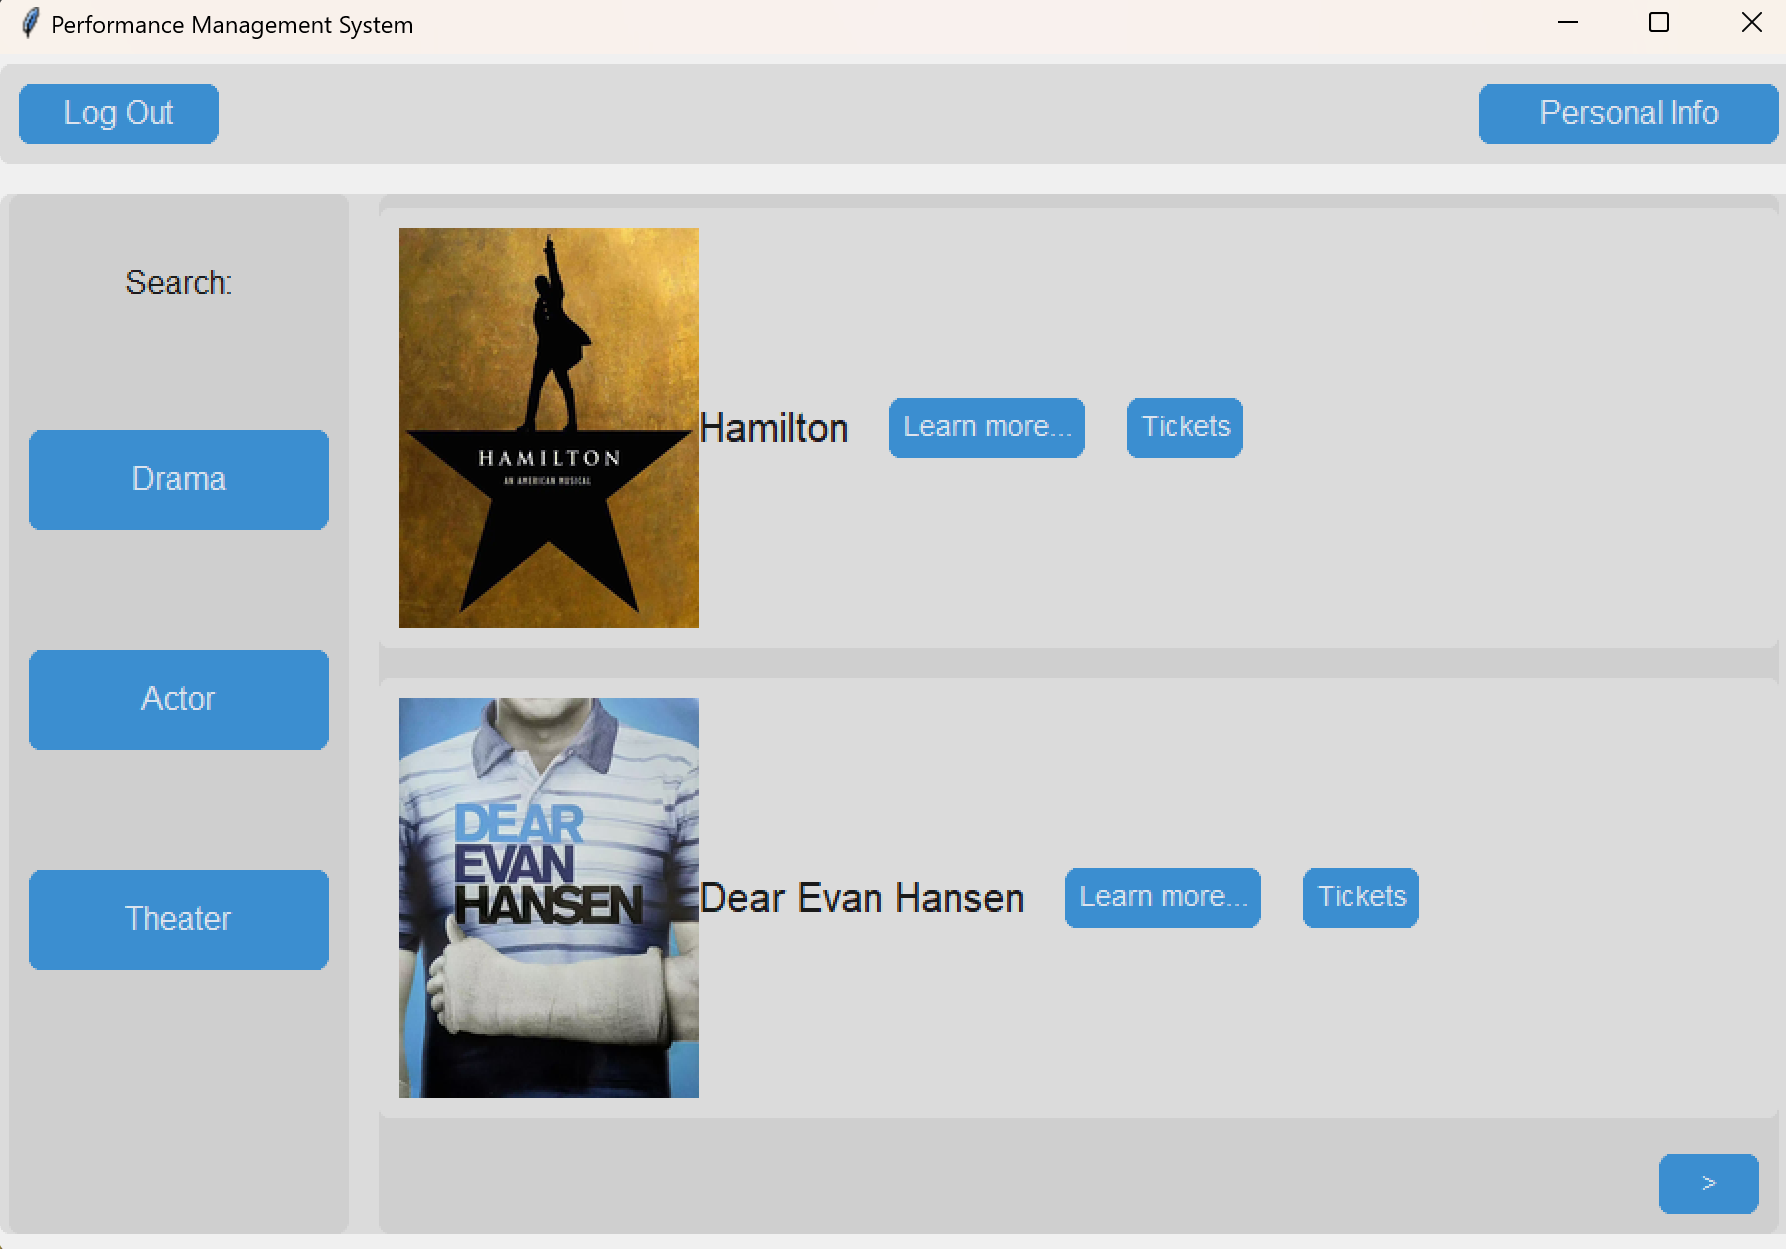
\includegraphics[width=\textwidth]{6.png}
        \caption{User dashboard}
        \label{Figure 6}
    \end{minipage}
    \hfill
    \begin{minipage}{0.48\textwidth}
        \centering
        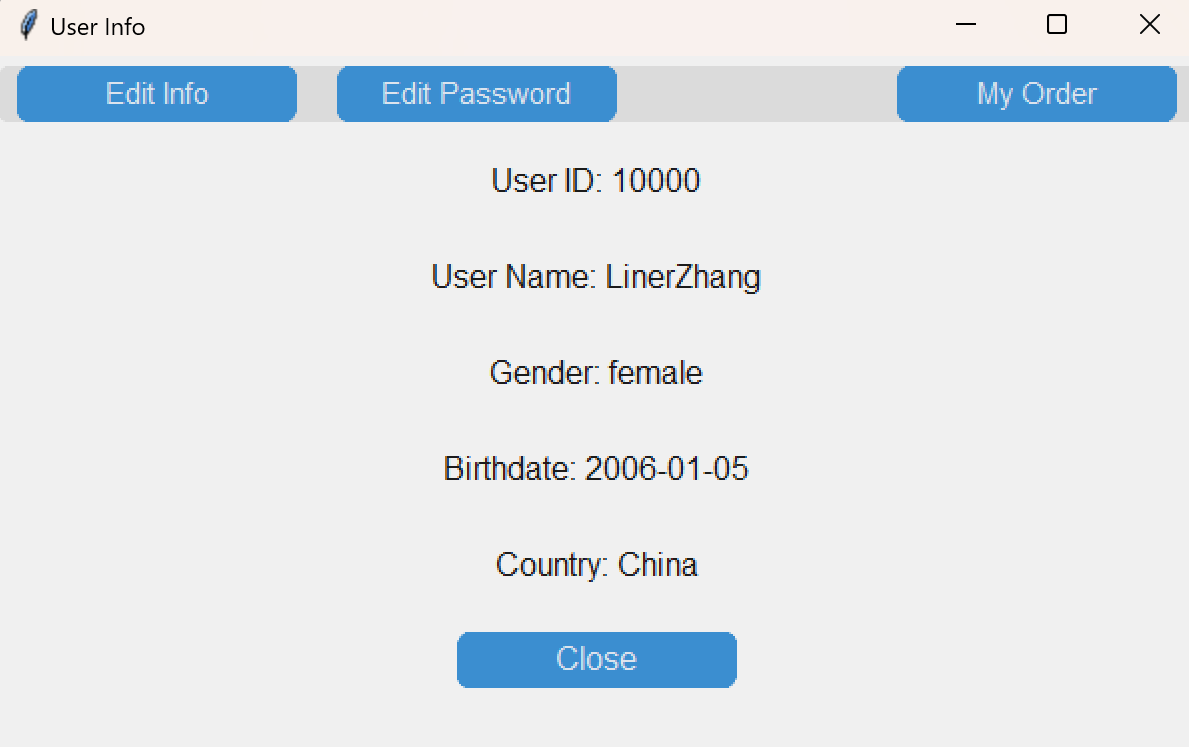
\includegraphics[width=\textwidth]{7.png}
        \caption{Personal info}
        \label{Figure 7}
    \end{minipage}
\end{figure}
\par In the Personal Info section, the user's personal information is displayed. Clicking 'Edit Personal Info' will open a new popup where the current information can be modified. Clicking 'Edit Password' will open a new popup prompting the user to enter both the old and new passwords, with the password only being updated if the old password is correct. Clicking 'My Orders' allows the user to view all the tickets they have purchased, along with the related viewing times and locations, providing convenience for the user.
\begin{figure}[H]
    \centering
    \begin{minipage}{0.45\textwidth}
        \centering
        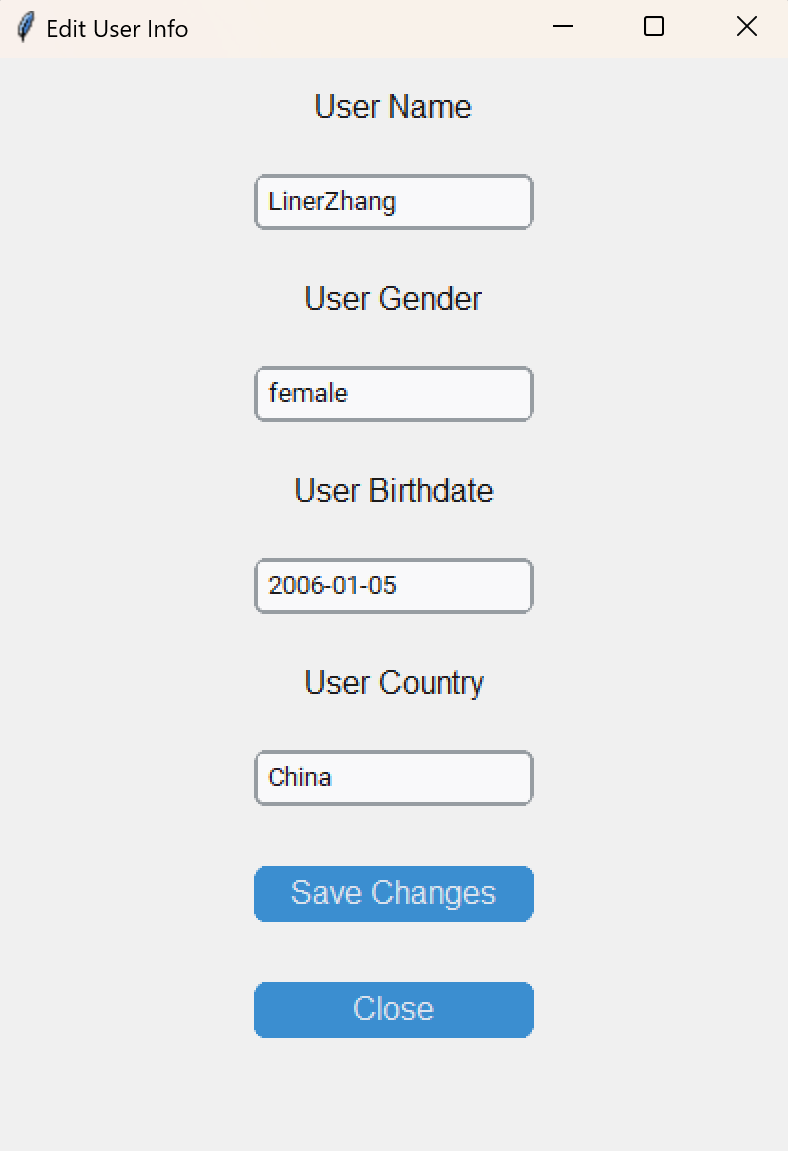
\includegraphics[width=\textwidth]{8.png}
        \caption{Edit info}
        \label{Figure 8}
    \end{minipage}
    \hfill
    \begin{minipage}{0.45\textwidth}
        \centering
        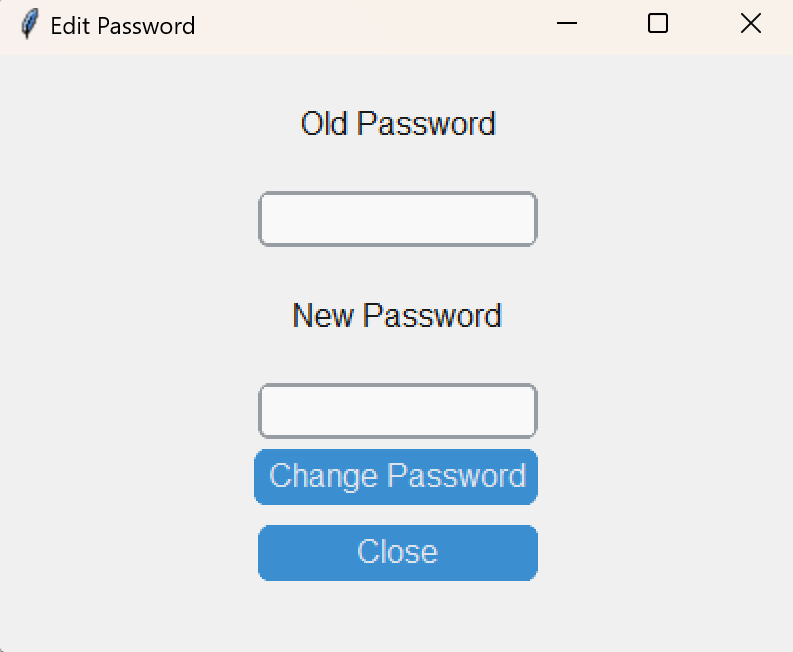
\includegraphics[width=\textwidth]{9.png}
        \caption{Edit password}
        \label{Figure 9}
    \end{minipage}
\end{figure}

\begin{figure}[H]
    \centering
    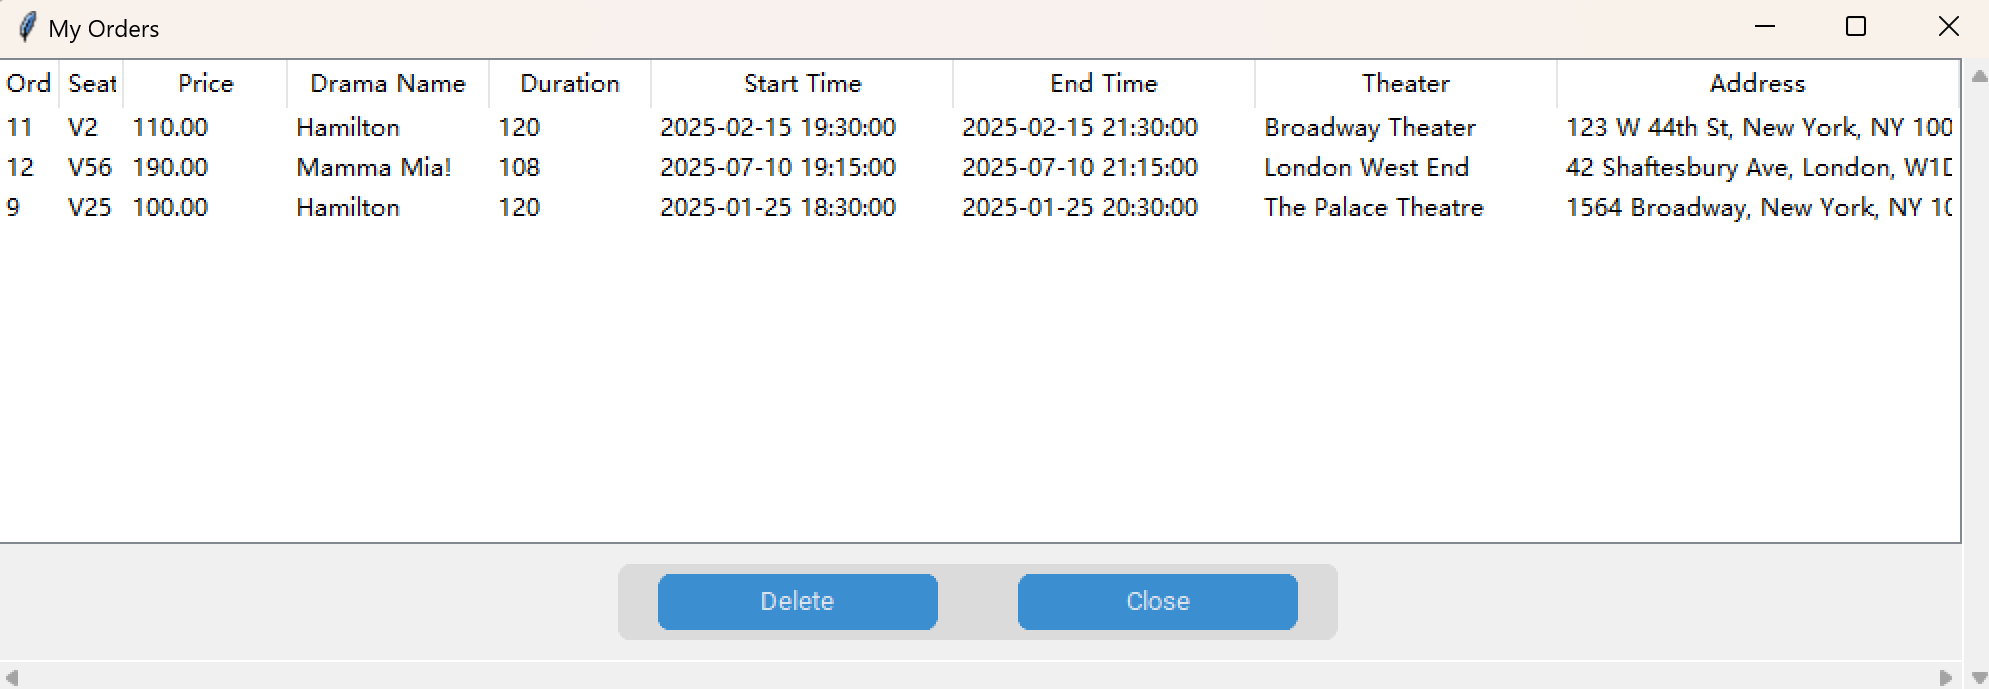
\includegraphics[width=0.7\textwidth]{10.png}
    \caption{My orders}
    \label{Figure 10}
\end{figure}

\subsubsection{Drama Display}
\par Clicking the 'Learn More' button of any drama that interests the user will display a brief summary of the drama's main content.\(Figure11-14\)
\begin{figure}[H]
    \centering
    \begin{minipage}{0.48\textwidth}
        \centering
        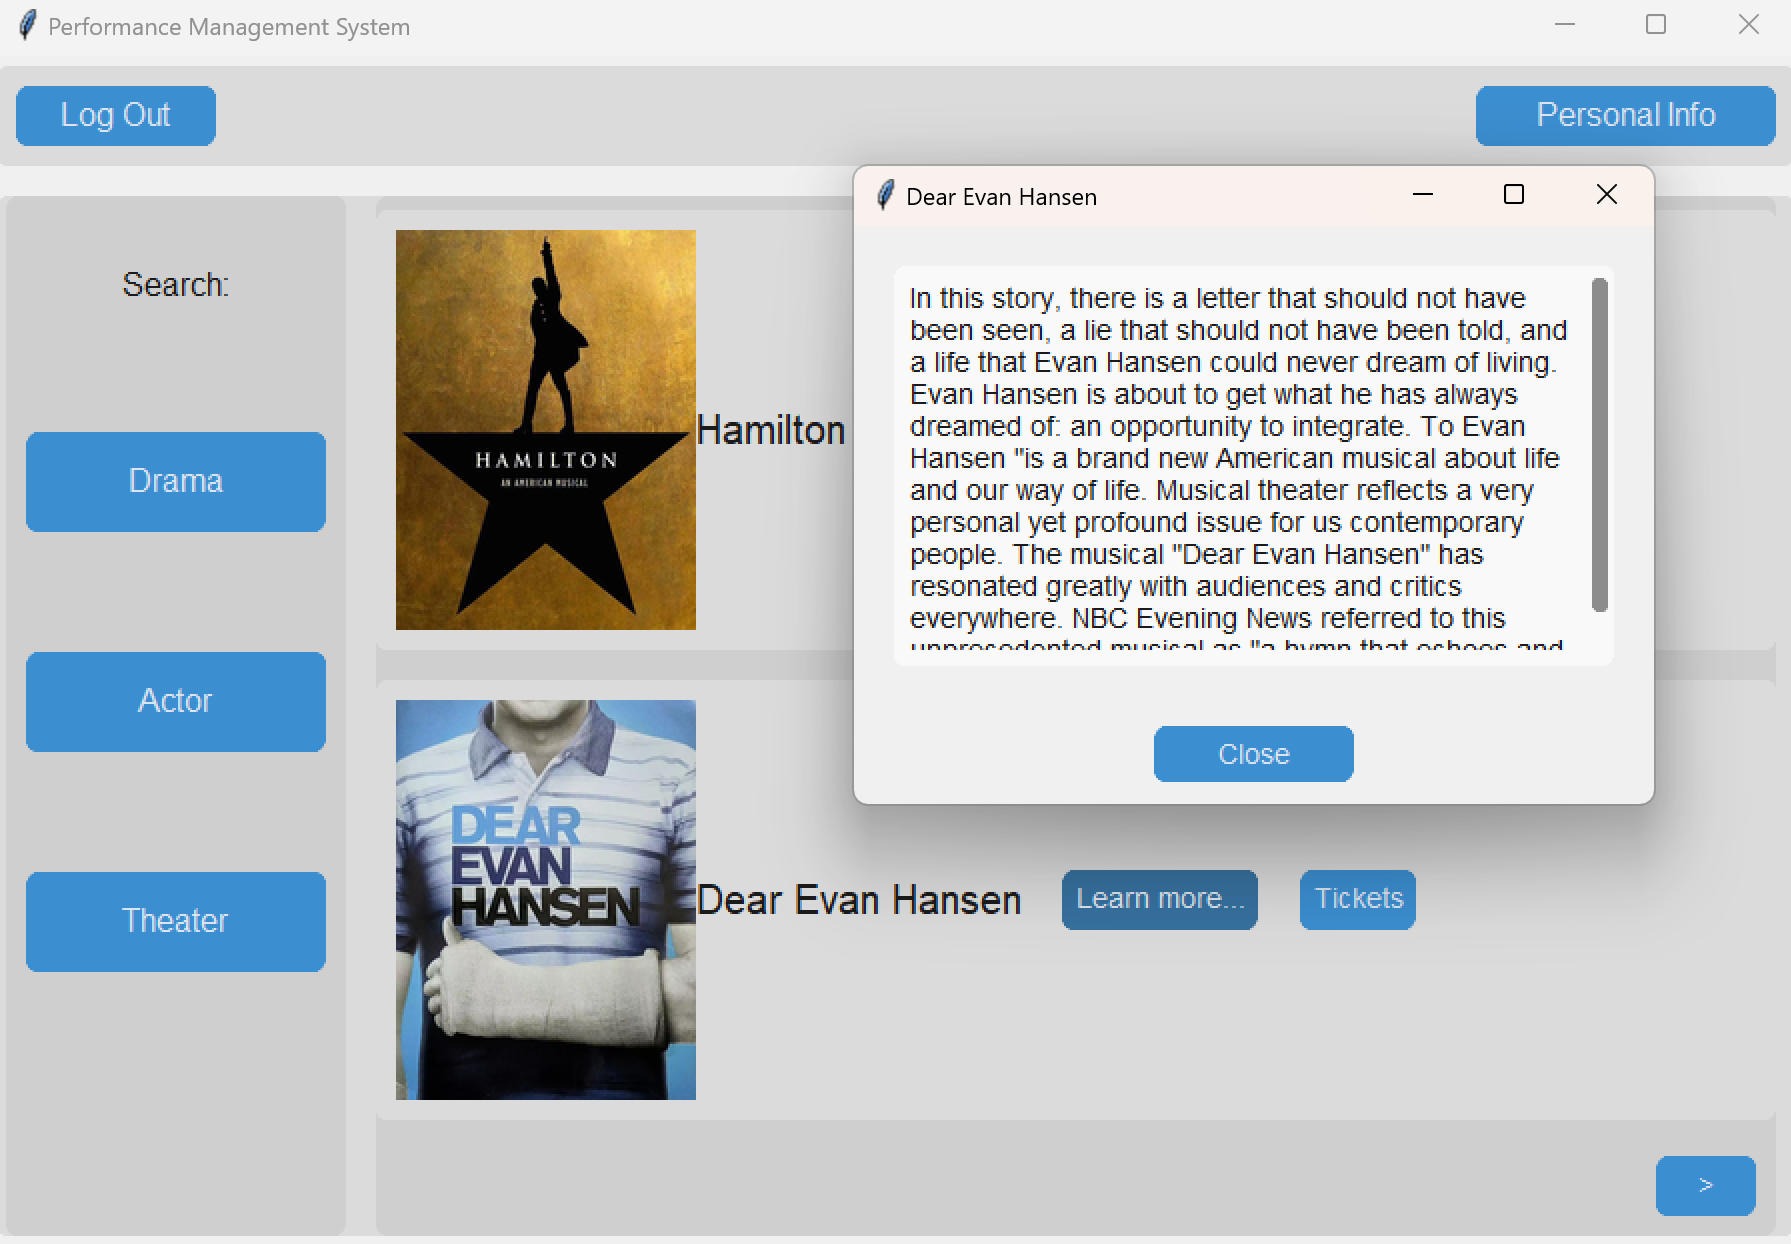
\includegraphics[width=\textwidth]{11.png}
        \caption{Learn more example} 
        \label{Figure 11}
    \end{minipage}
    \hfill
    \begin{minipage}{0.48\textwidth}
        \centering
        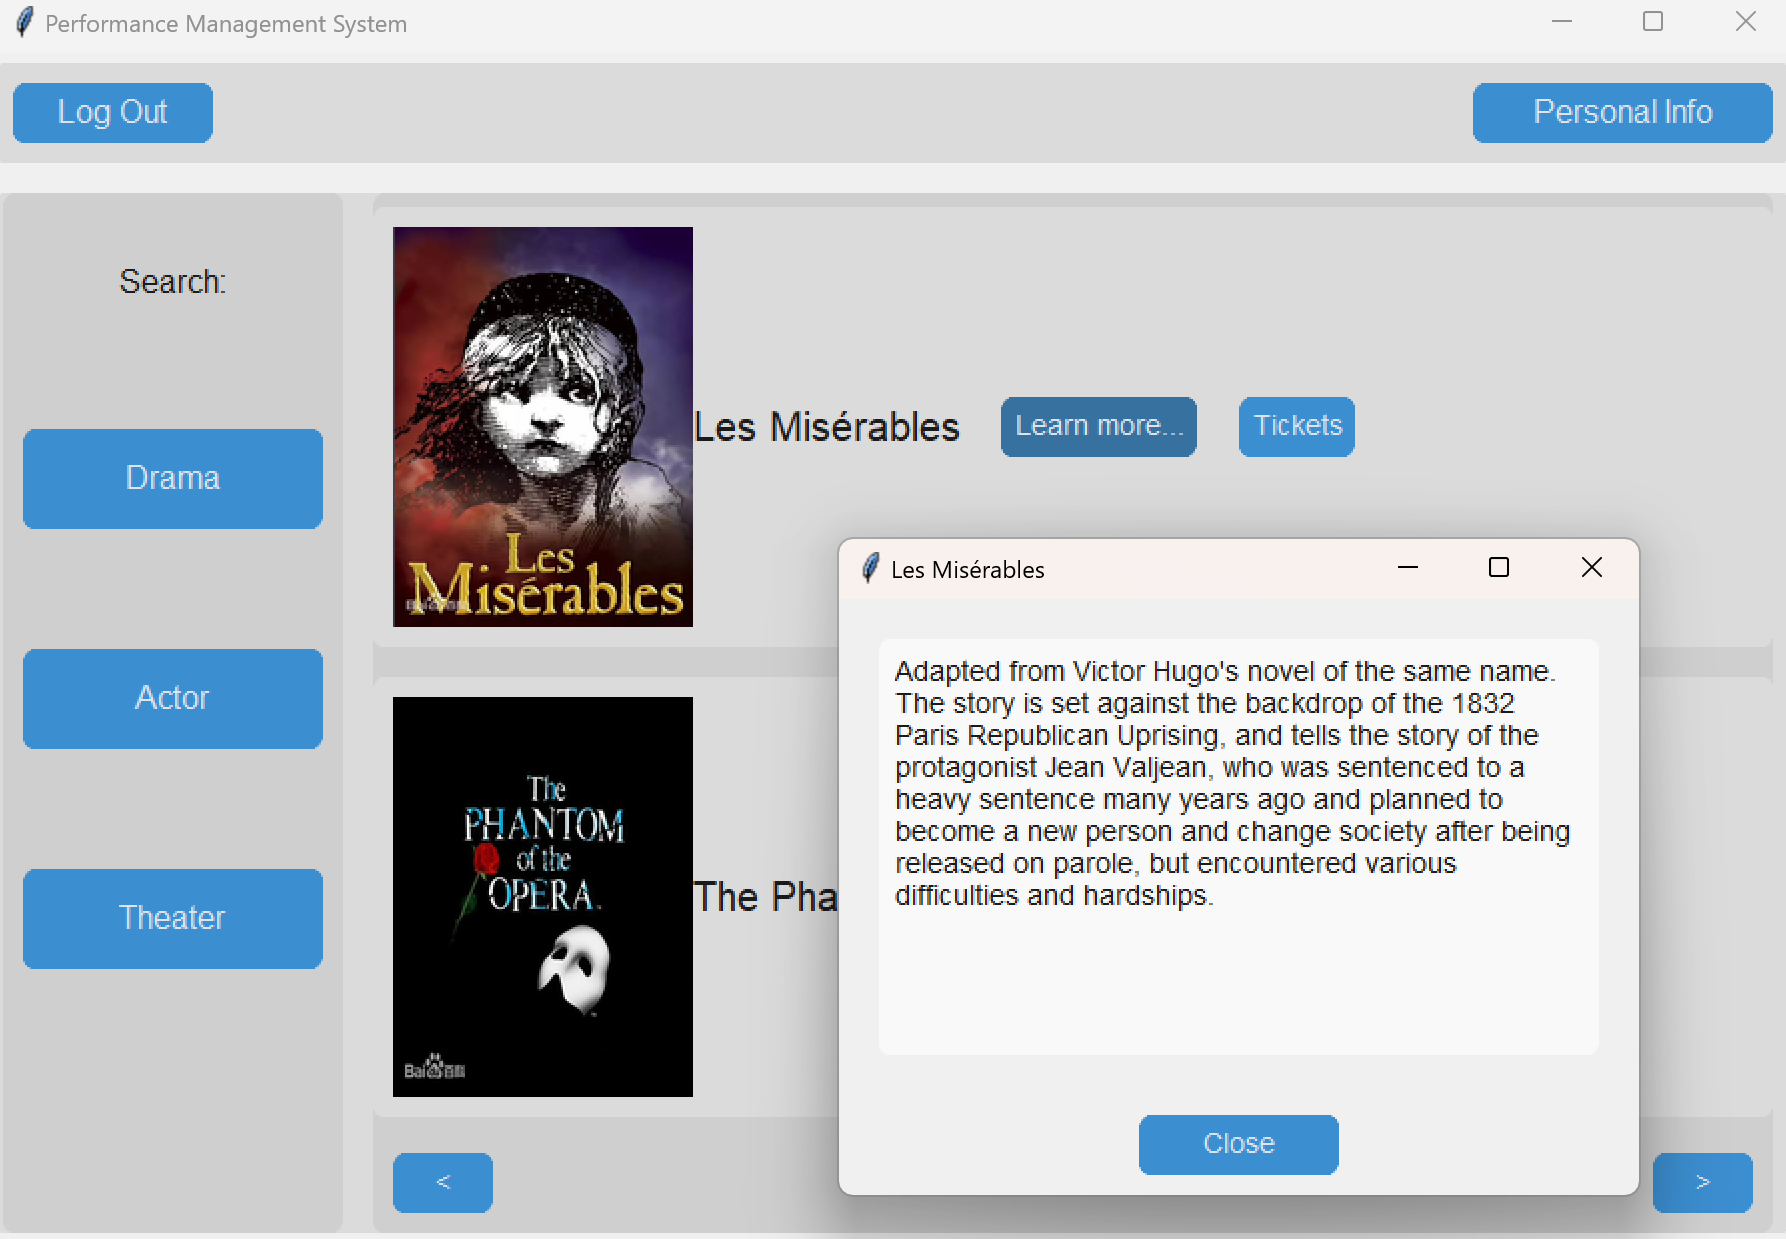
\includegraphics[width=\textwidth]{12.png}
        \caption{Learn more example}
        \label{Figure 12}
    \end{minipage}
\end{figure}

\par When displaying tickets, the user can choose the sorting method and type for the display. After clicking on the ticket they wish to purchase, clicking 'Buy It Now' will display the complete order details, allowing the user to confirm the purchase.
\begin{figure}[H]
    \centering
    \begin{minipage}{0.48\textwidth}
        \centering
        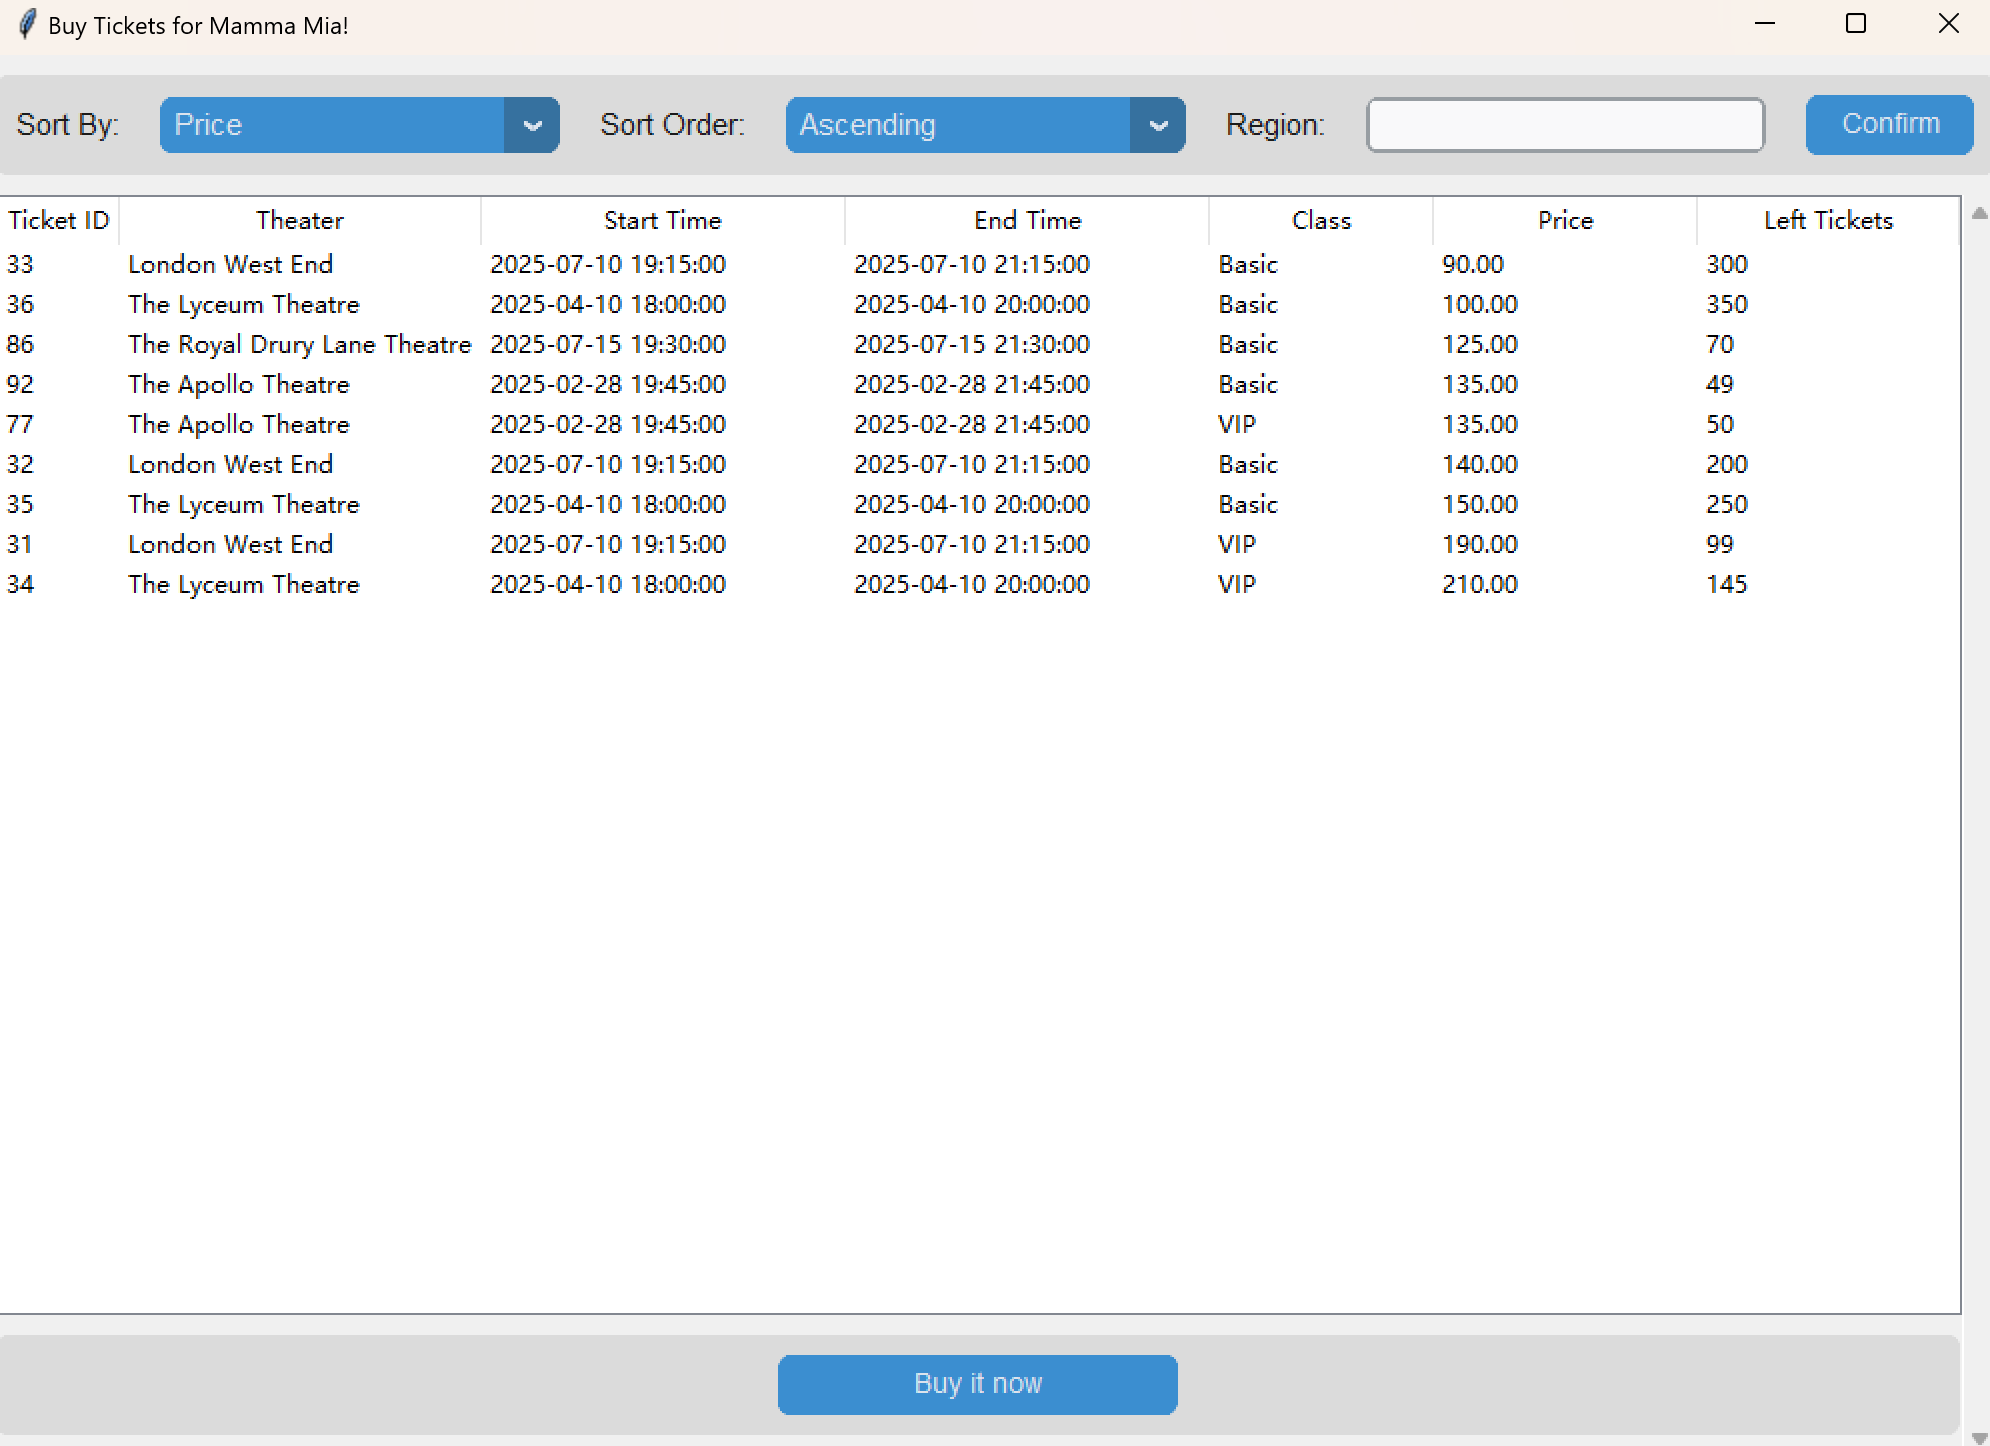
\includegraphics[width=\textwidth]{13.png}
        \caption{Tickets example} 
        \label{Figure 13}
    \end{minipage}
    \hfill
    \begin{minipage}{0.48\textwidth}
        \centering
        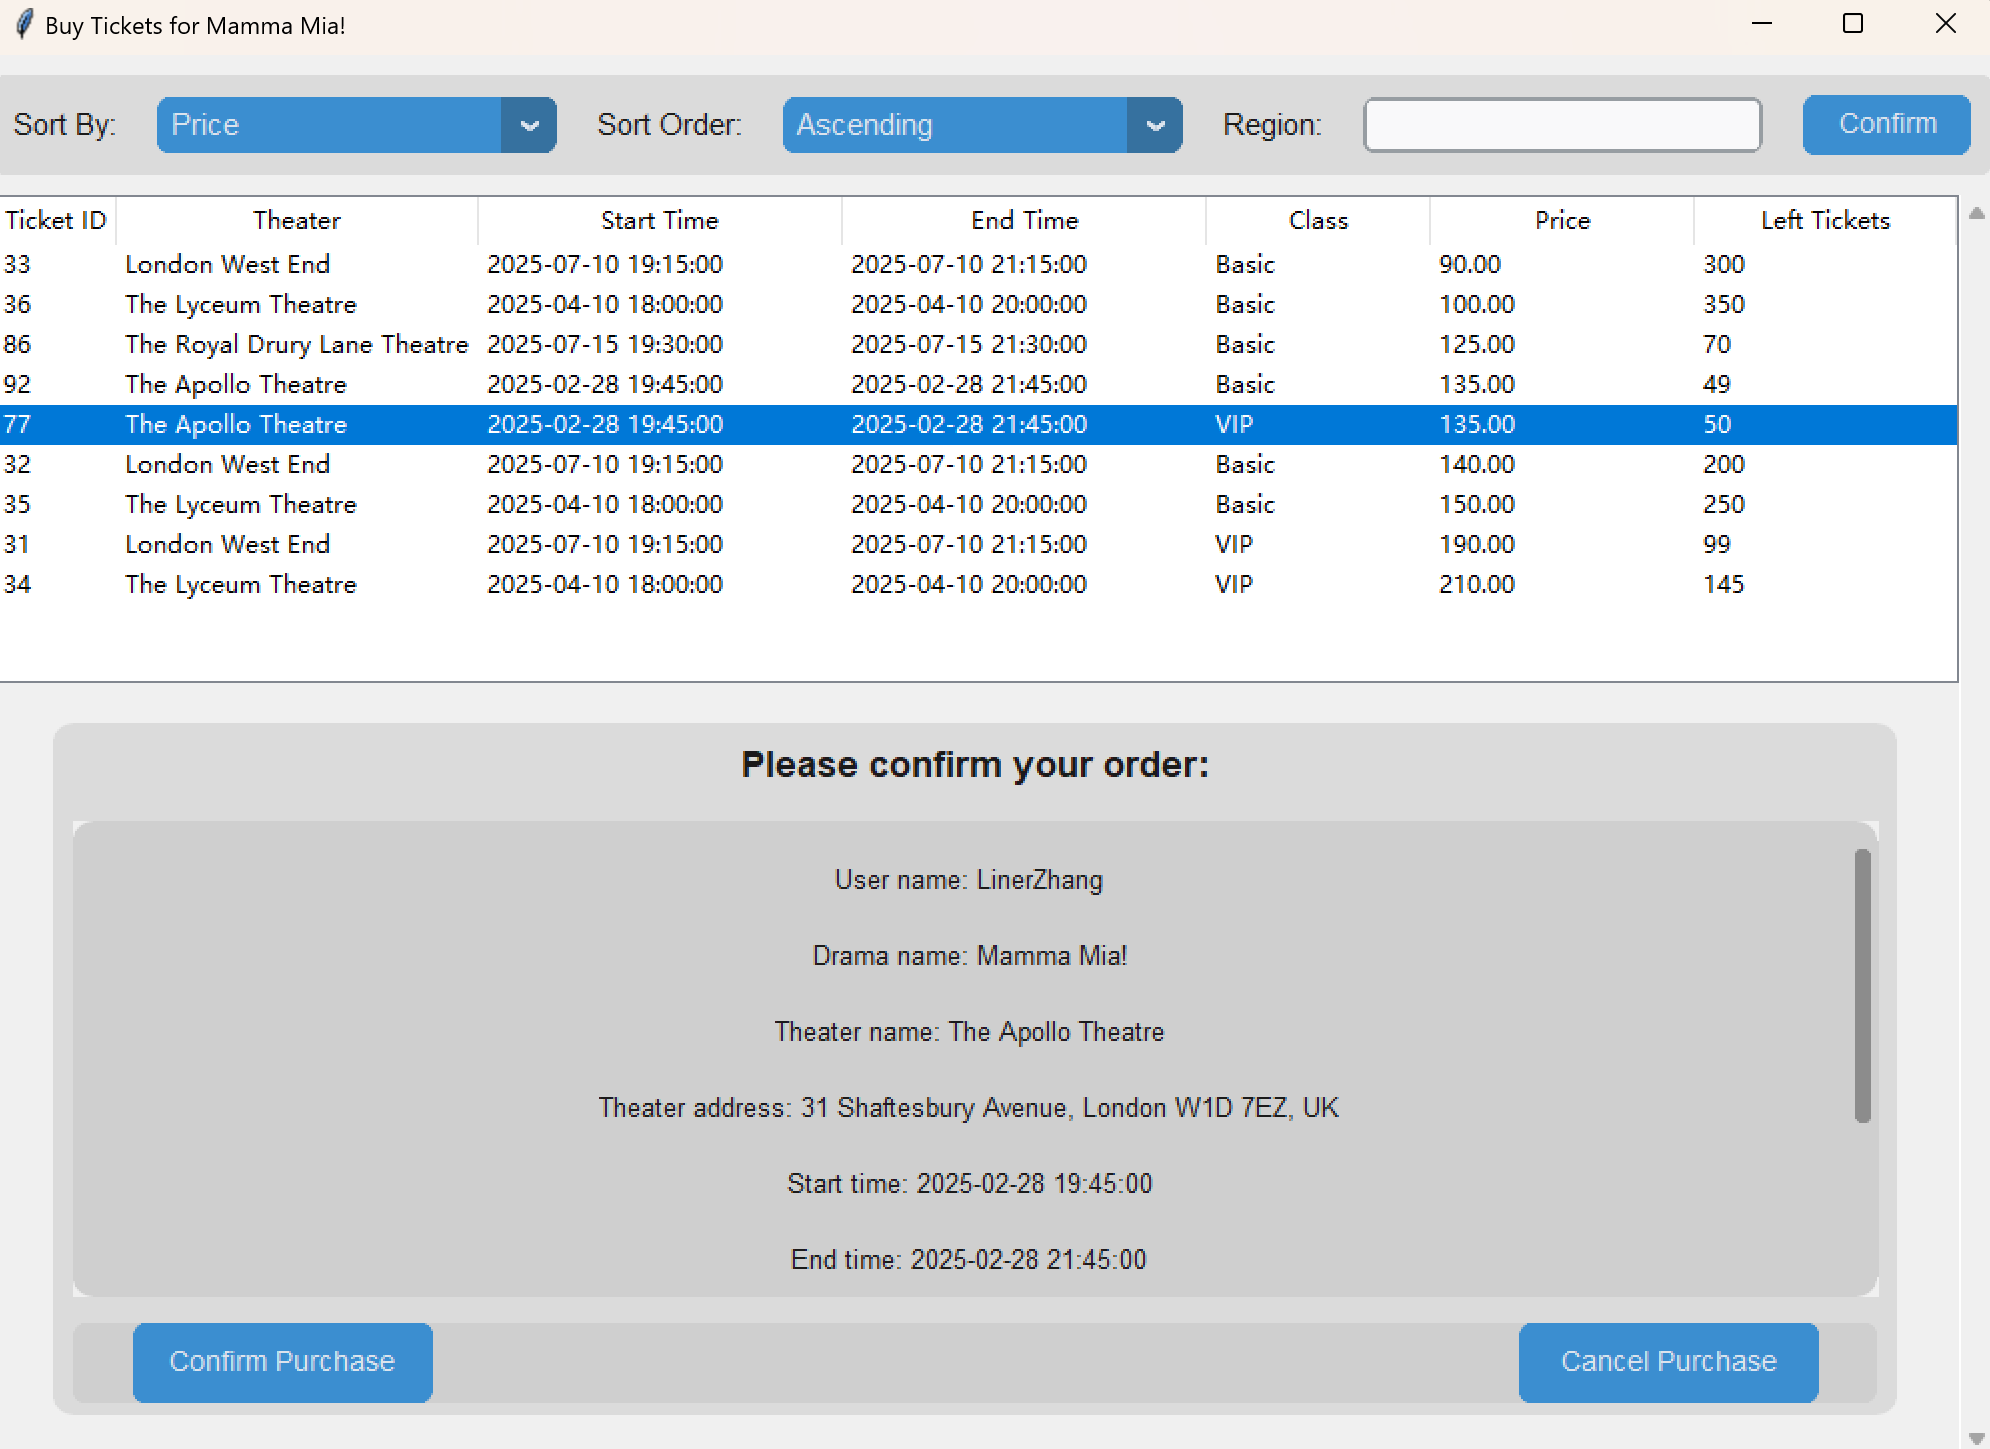
\includegraphics[width=\textwidth]{14.png}
        \caption{Buy it now}
        \label{Figure 14}
    \end{minipage}
\end{figure}

\subsubsection{Actor Display}
\par The process is the same as before, so it is omitted.\(Figure15-18\)
\begin{figure}[H]
    \centering
    \begin{minipage}{0.48\textwidth}
        \centering
        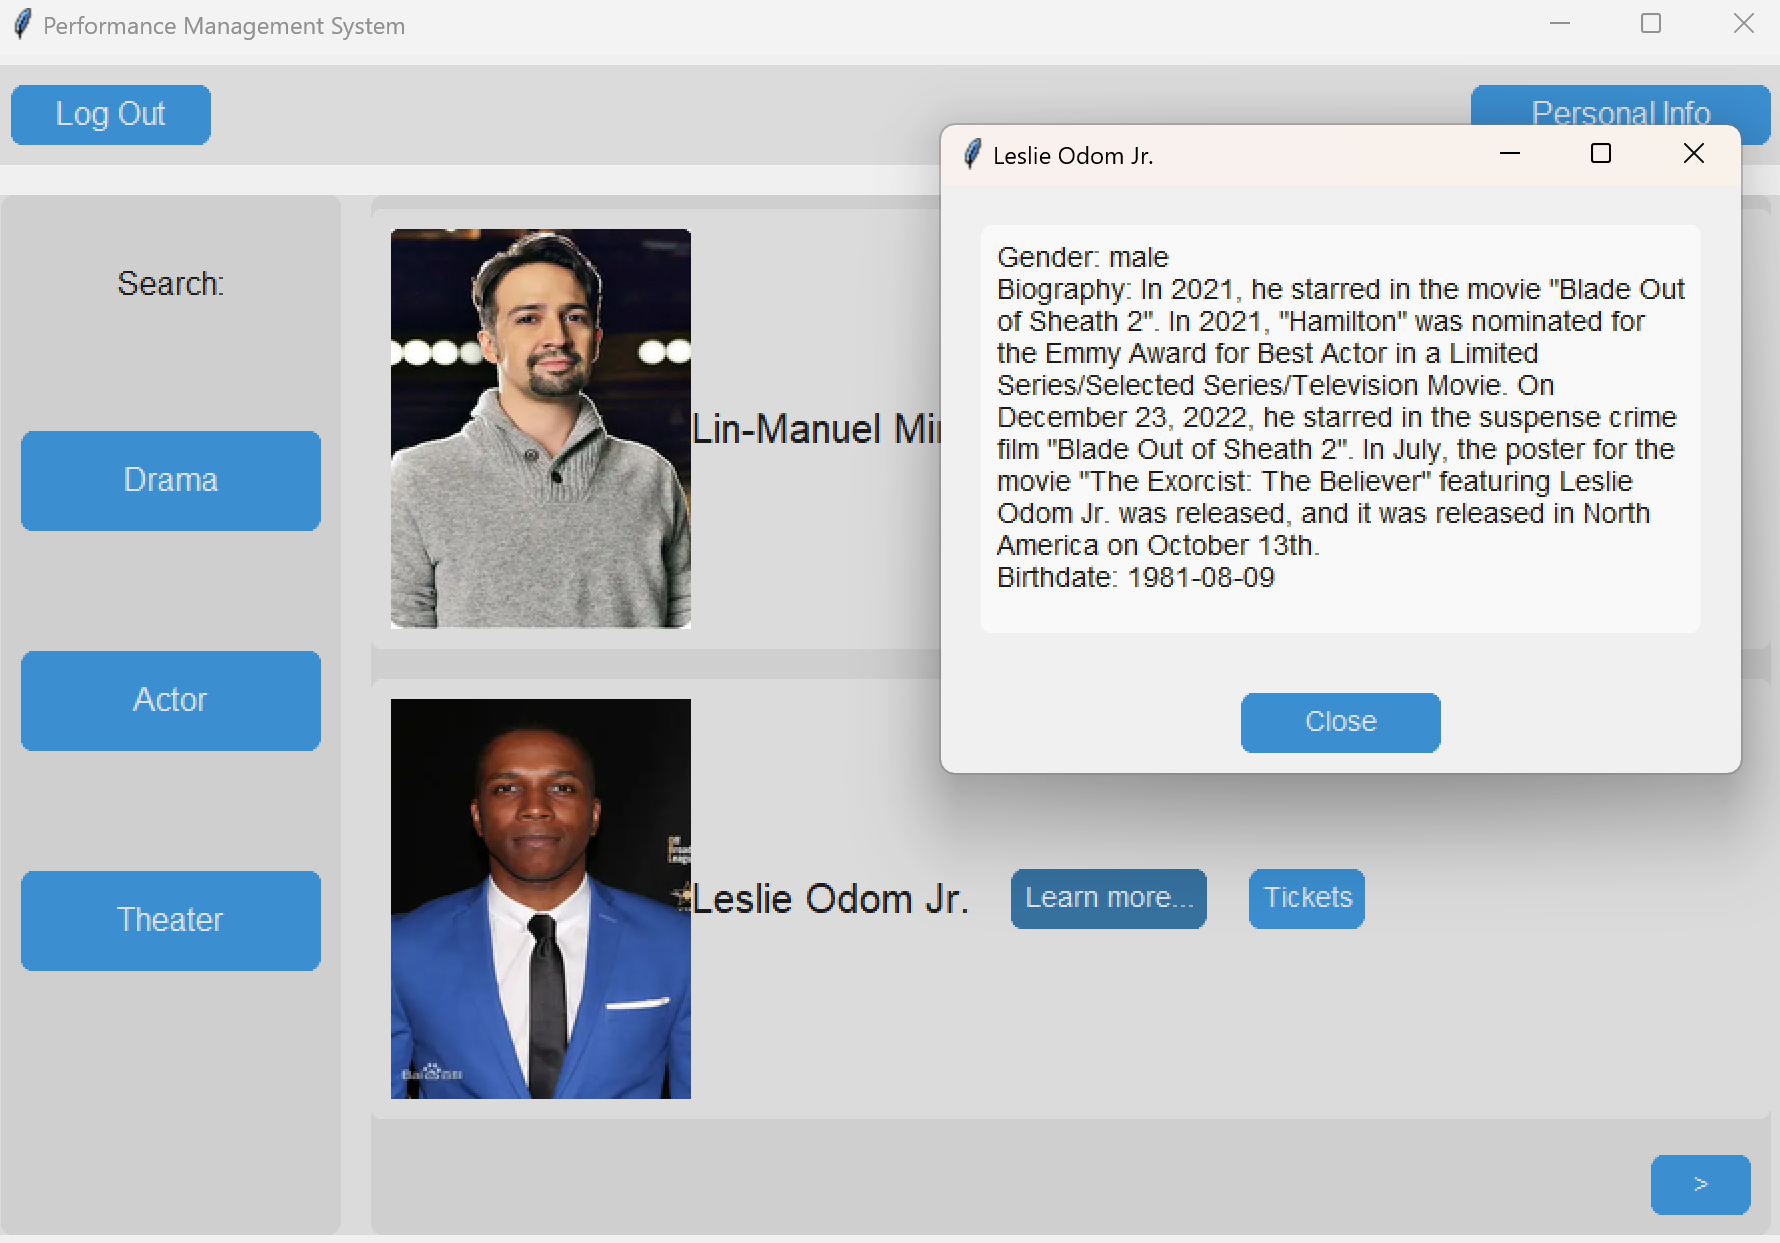
\includegraphics[width=\textwidth]{15.png}
        \caption{Learn more example} 
        \label{Figure 15}
    \end{minipage}
    \hfill
    \begin{minipage}{0.48\textwidth}
        \centering
        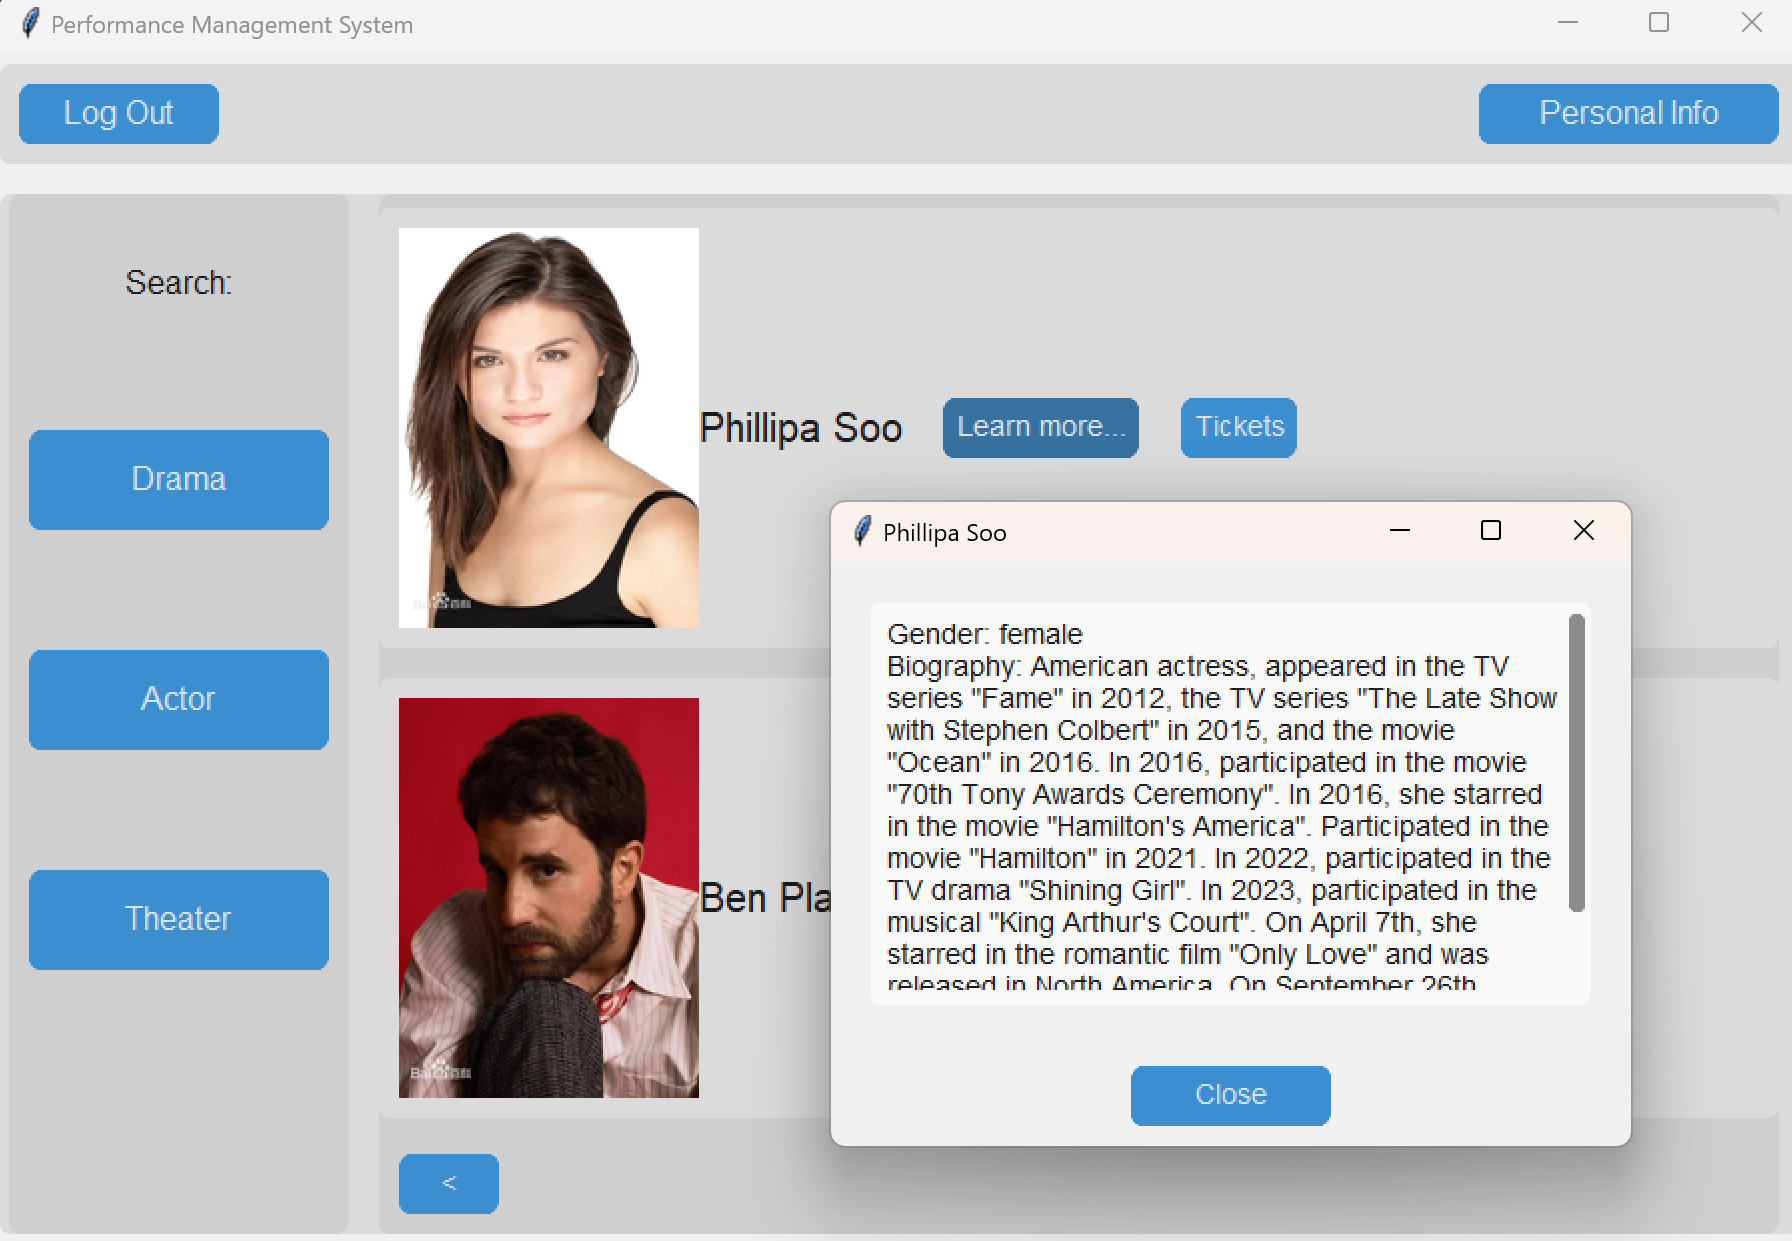
\includegraphics[width=\textwidth]{16.png}
        \caption{Learn more example}
        \label{Figure 16}
    \end{minipage}
\end{figure}

\begin{figure}[H]
    \centering
    \begin{minipage}{0.48\textwidth}
        \centering
        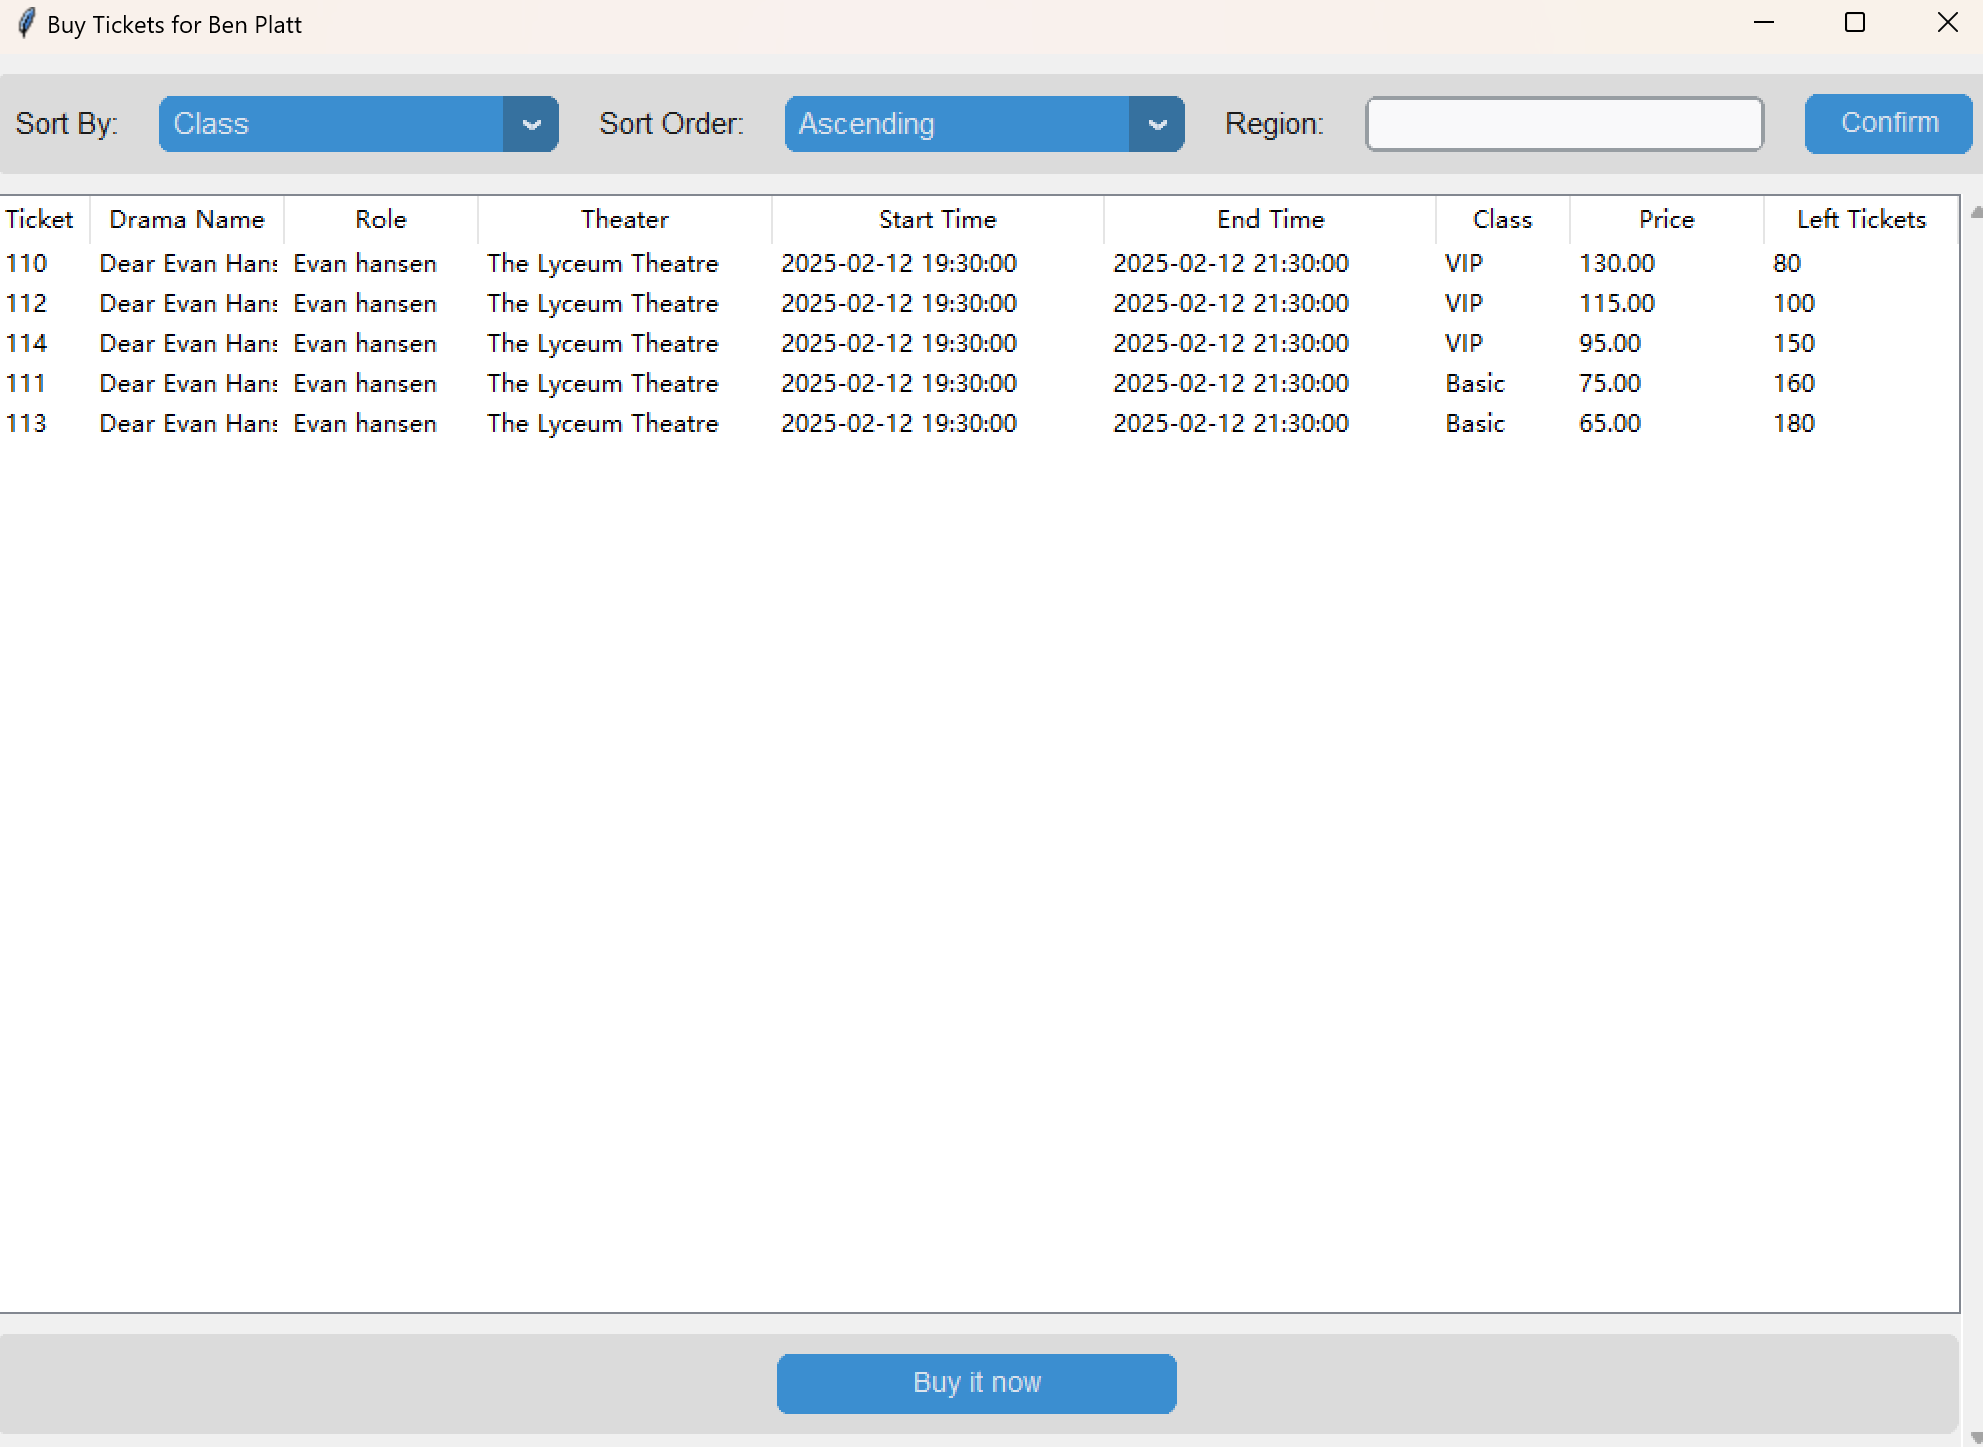
\includegraphics[width=\textwidth]{17.png}
        \caption{Tickets example} 
        \label{Figure 17}
    \end{minipage}
    \hfill
    \begin{minipage}{0.48\textwidth}
        \centering
        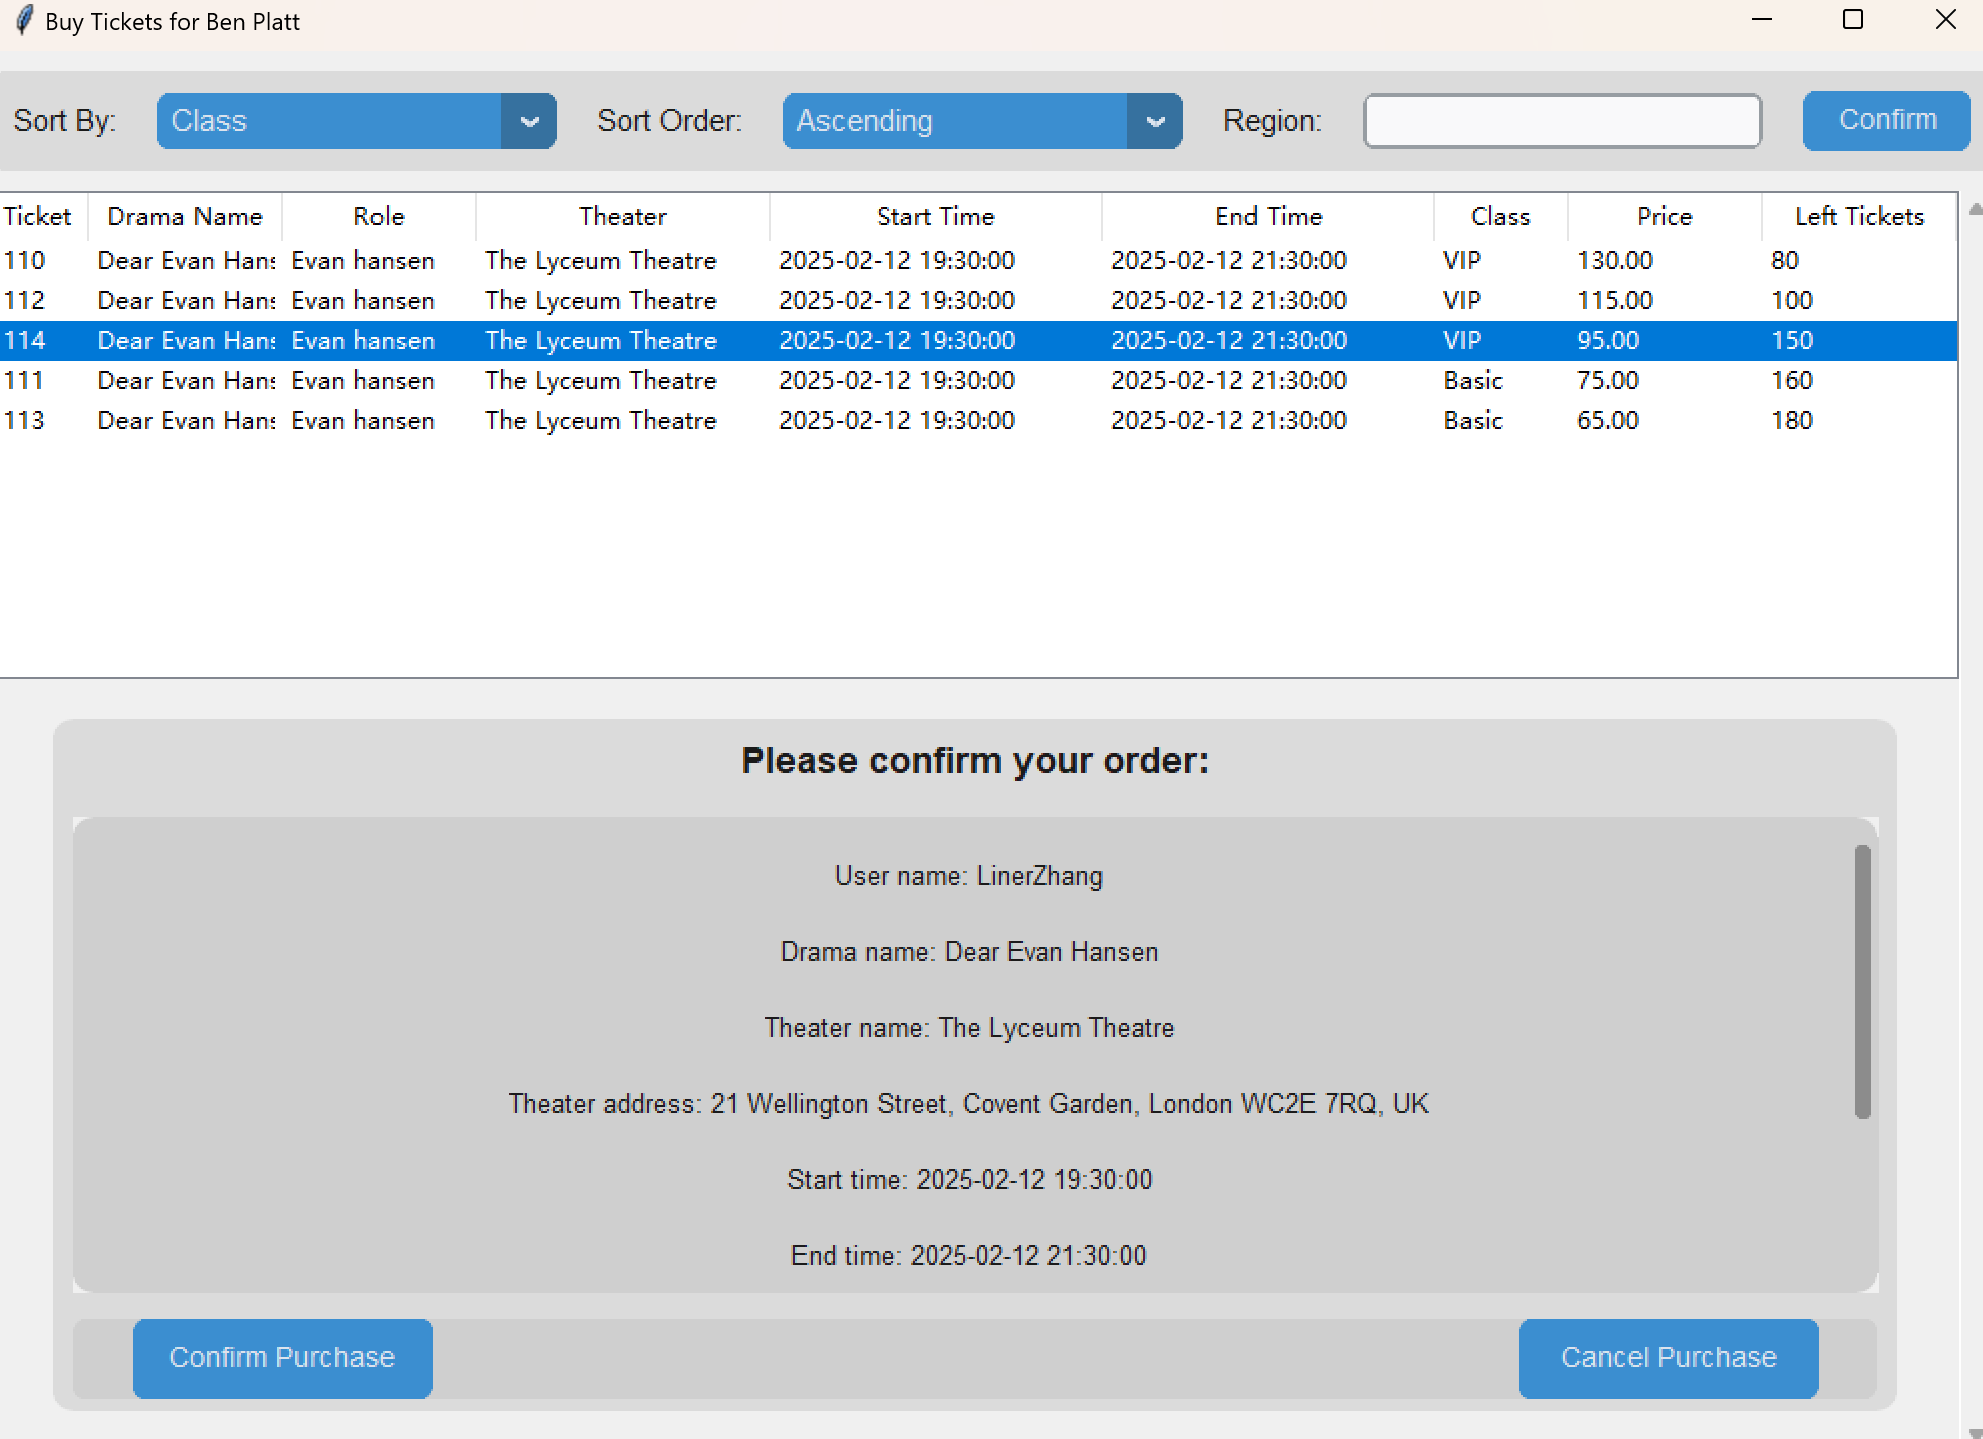
\includegraphics[width=\textwidth]{18.png}
        \caption{Buy it now}
        \label{Figure 18}
    \end{minipage}
\end{figure}

\subsubsection{Theater Display}
\par The process is the same as before, so it is omitted.\(Figure19-22\)
\begin{figure}[H]
    \centering
    \begin{minipage}{0.48\textwidth}
        \centering
        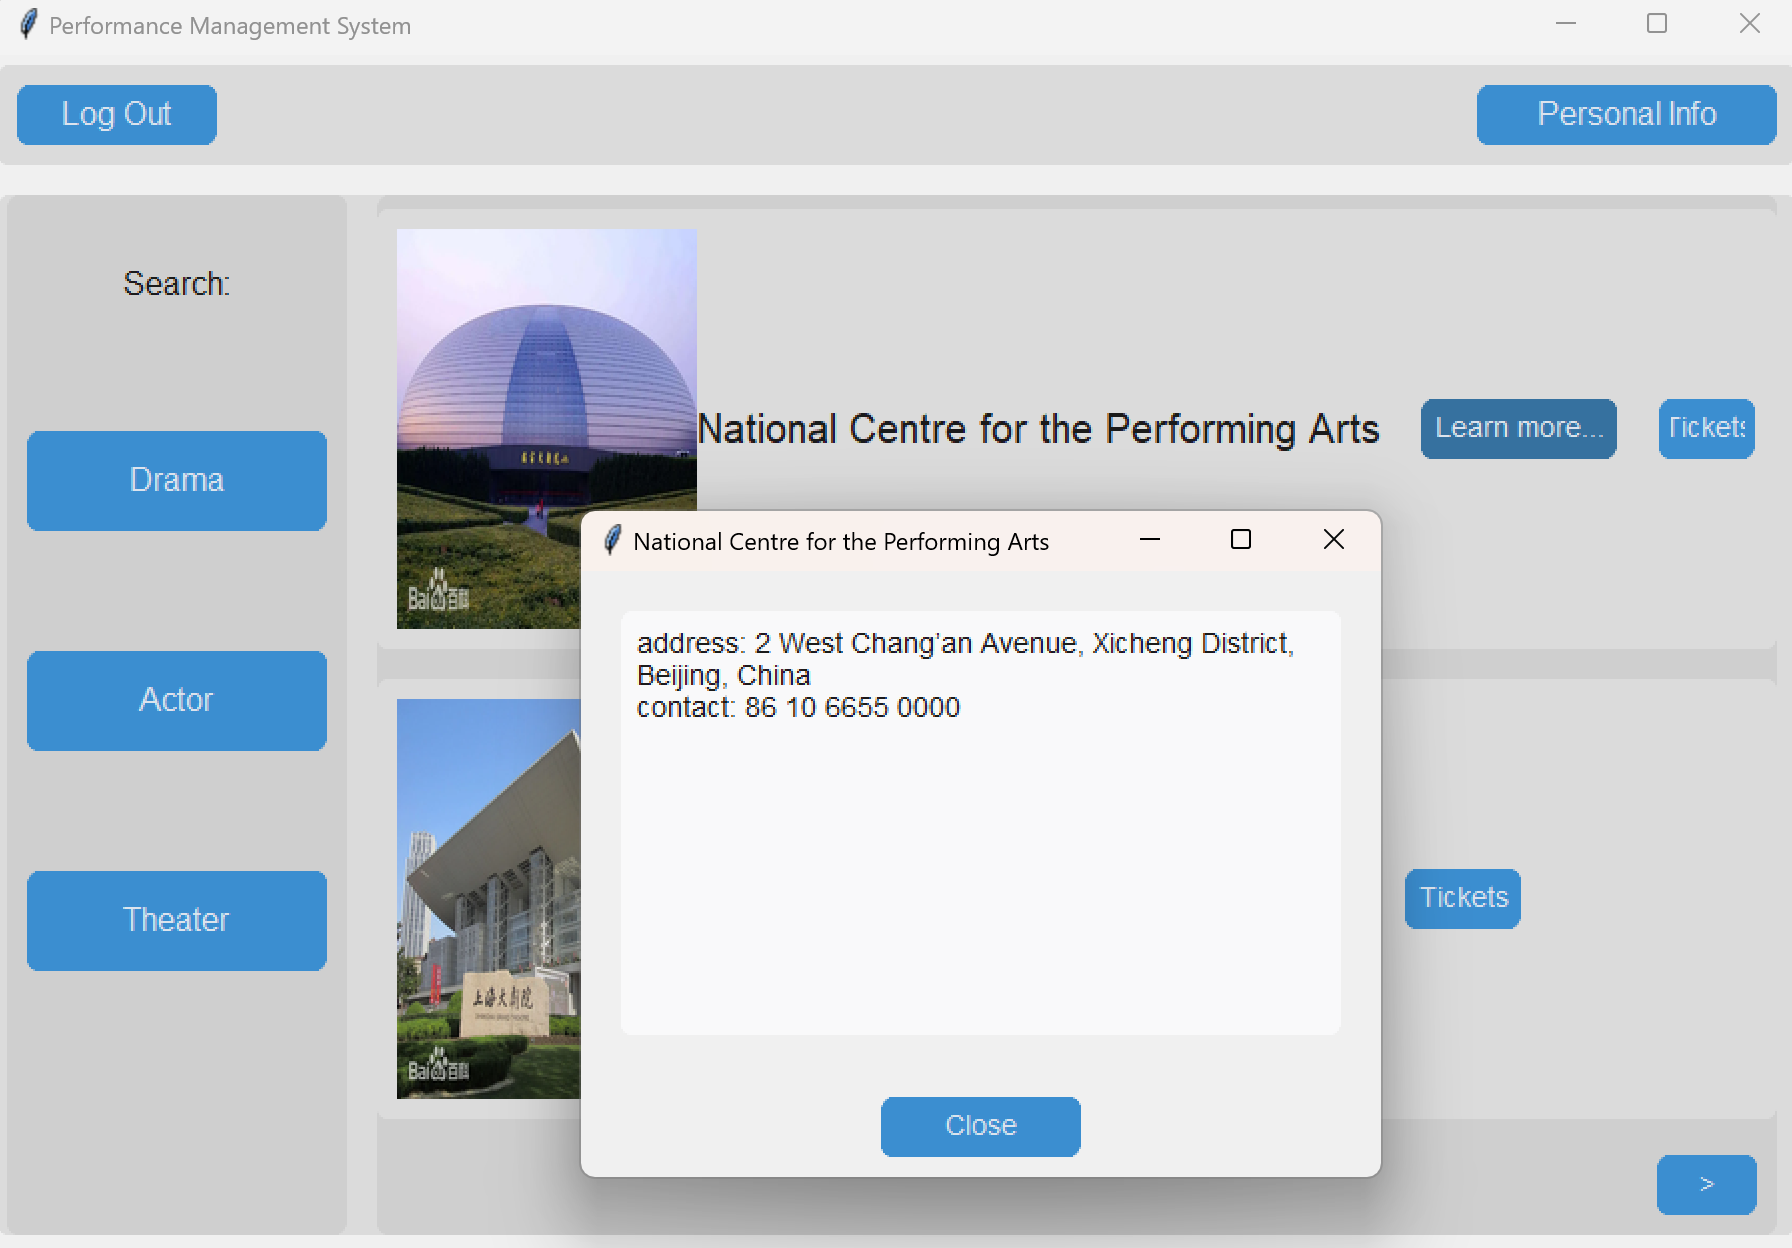
\includegraphics[width=\textwidth]{19.png}
        \caption{Learn more example} 
        \label{Figure 19}
    \end{minipage}
    \hfill
    \begin{minipage}{0.48\textwidth}
        \centering
        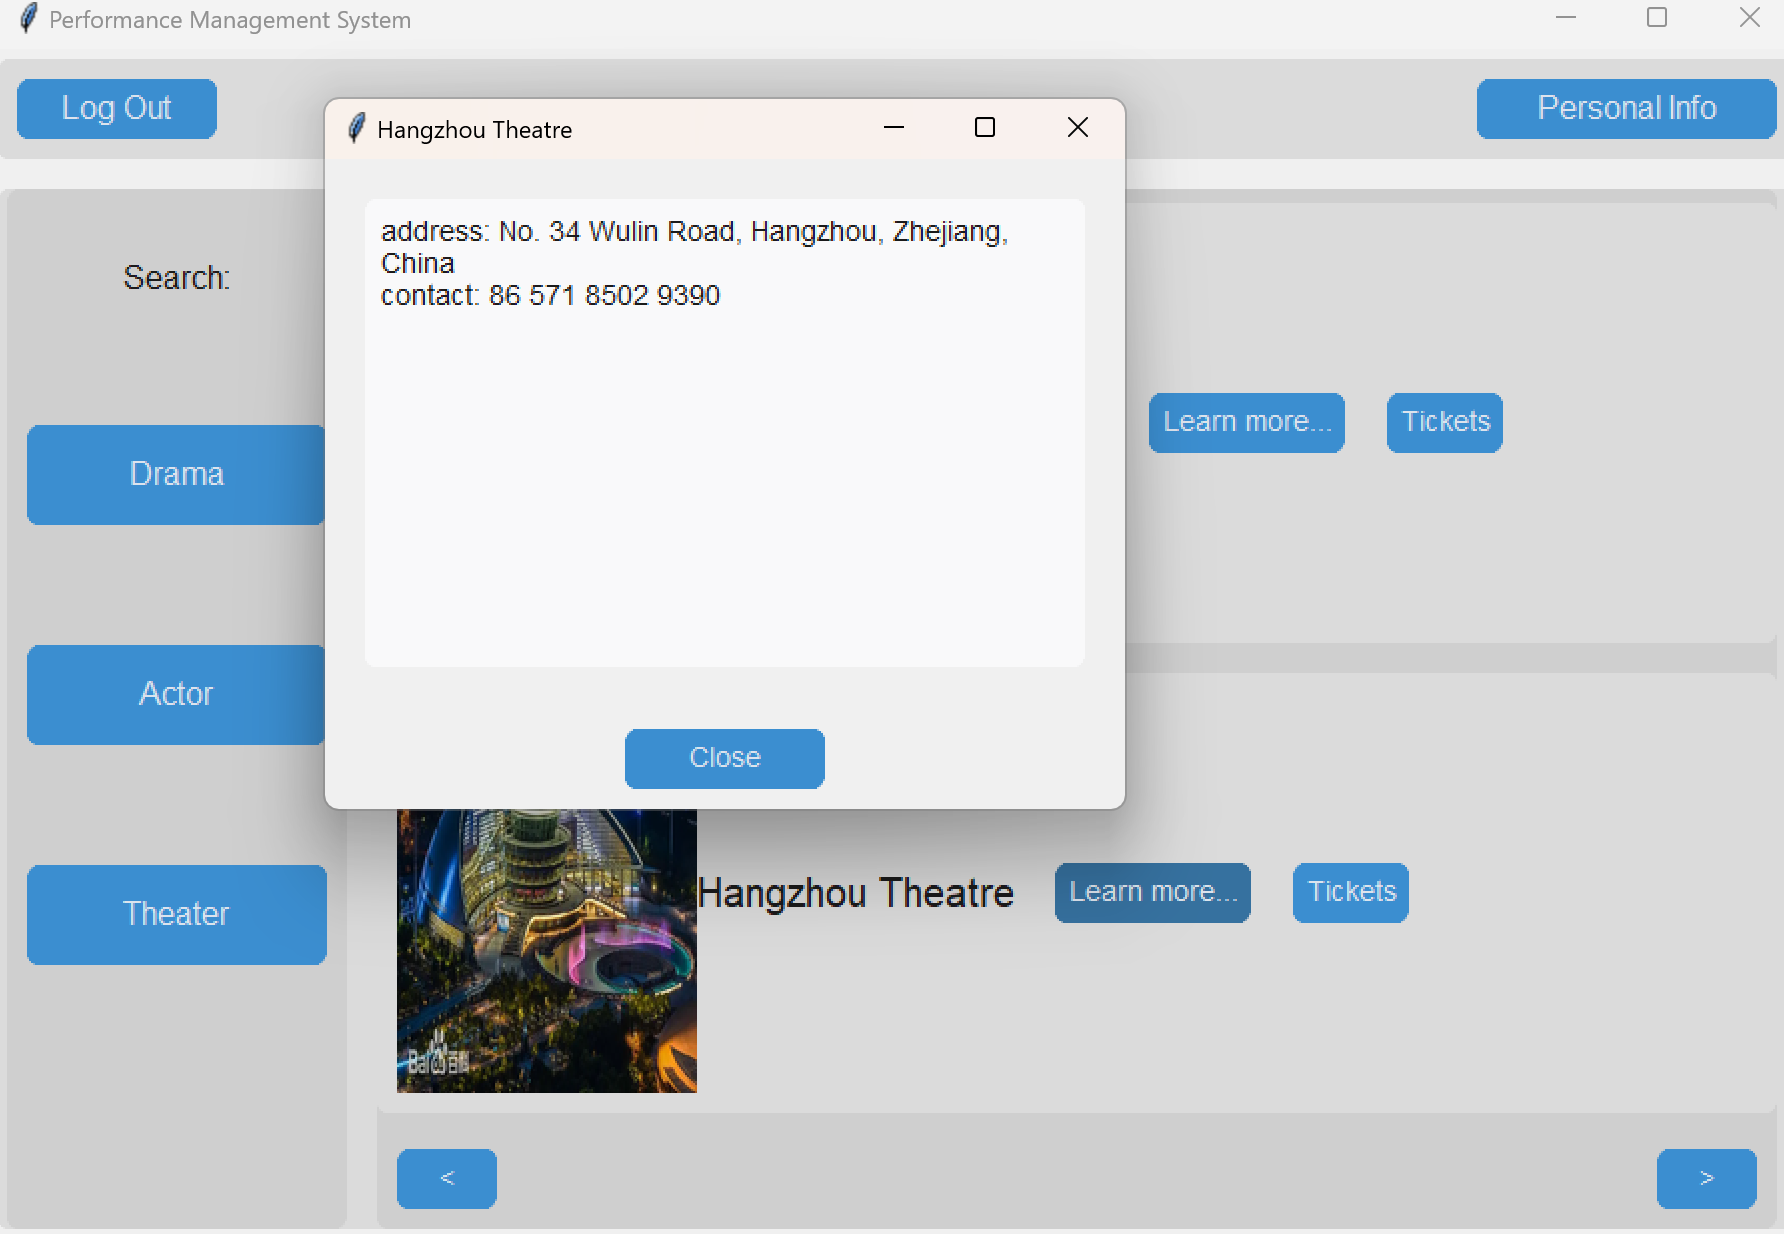
\includegraphics[width=\textwidth]{20.png}
        \caption{Learn more example}
        \label{Figure 20}
    \end{minipage}
\end{figure}

\begin{figure}[H]
    \centering
    \begin{minipage}{0.48\textwidth}
        \centering
        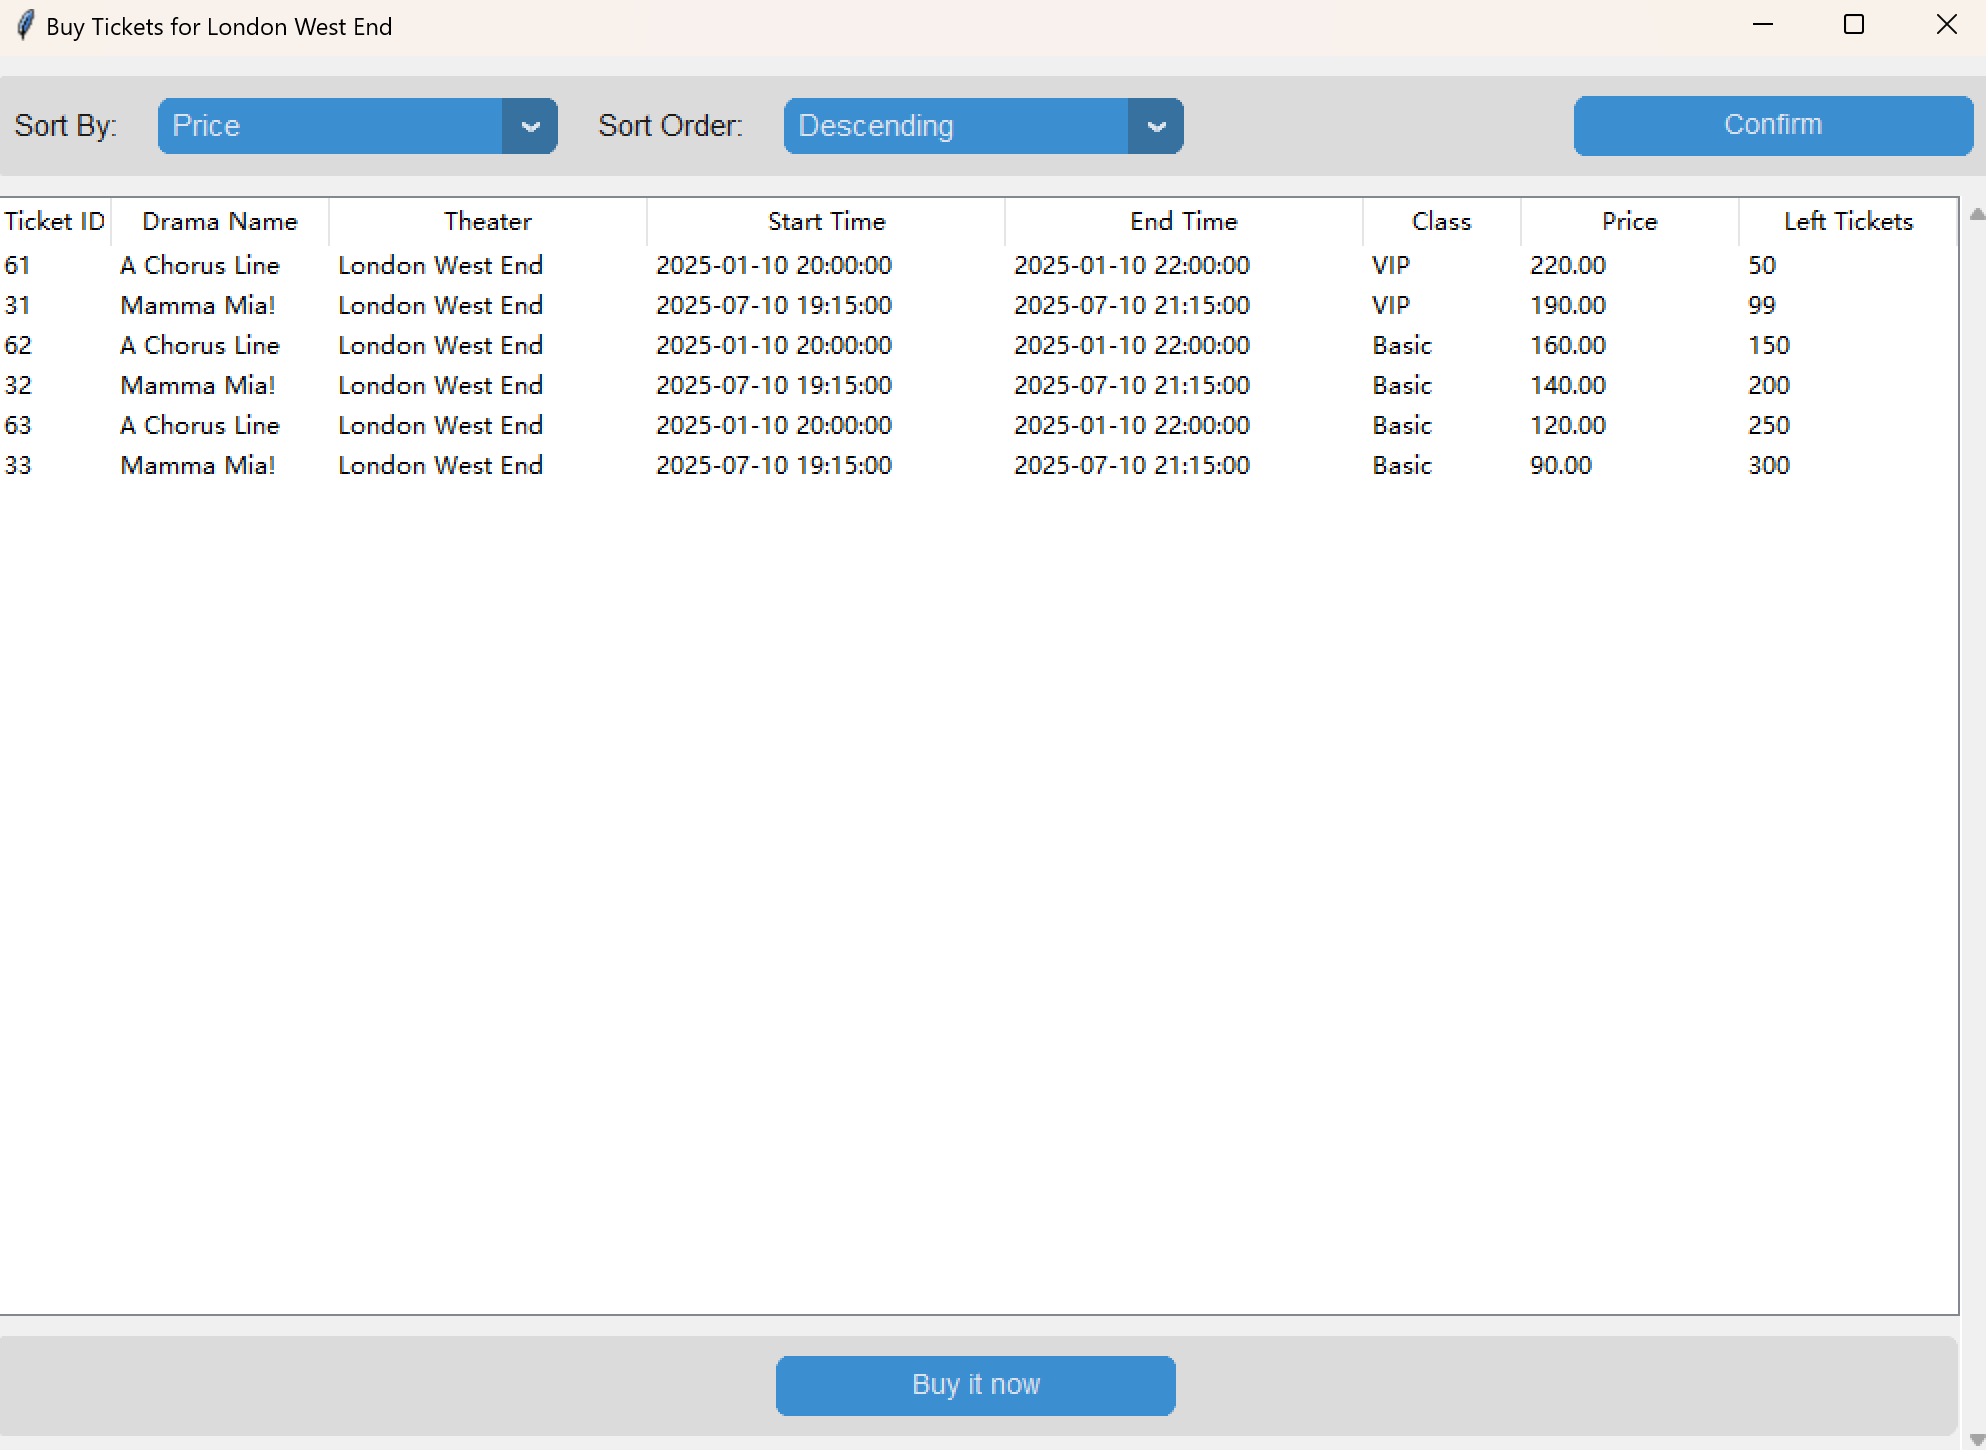
\includegraphics[width=\textwidth]{21.png}
        \caption{Tickets example} 
        \label{Figure 21}
    \end{minipage}
    \hfill
    \begin{minipage}{0.48\textwidth}
        \centering
        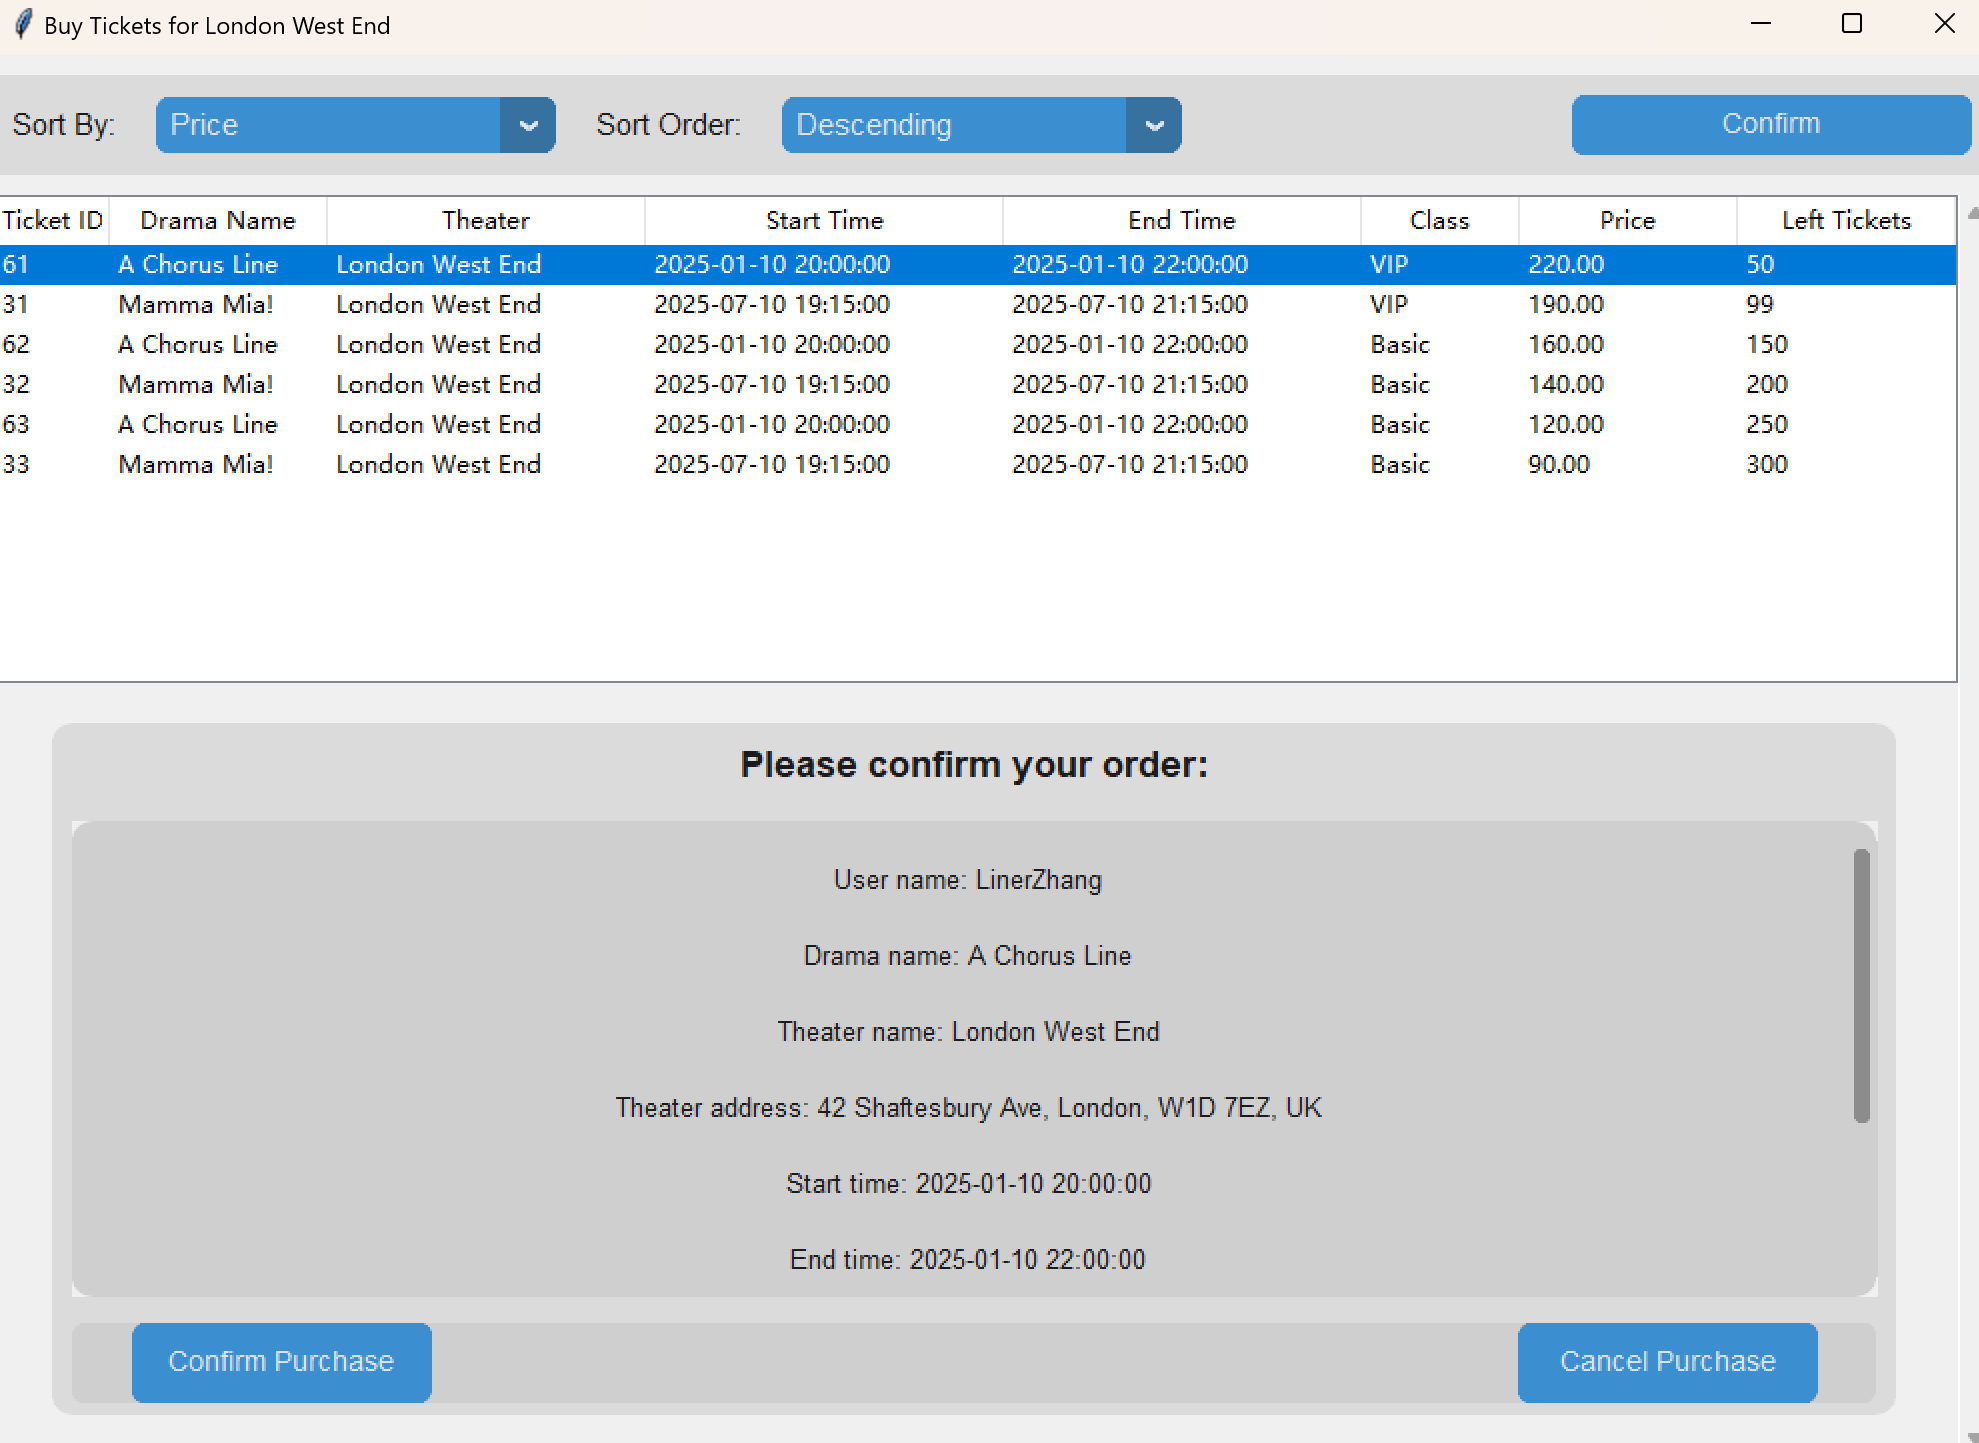
\includegraphics[width=\textwidth]{22.png}
        \caption{Buy it now}
        \label{Figure 22}
    \end{minipage}
\end{figure}

\subsection{Staff Usage}
\par The login process is the same as before, except without the registration option, so it is omitted.
available staff account:
\begin{itemize}
    \item Work ID: 10000
    \item Password: 123456
\end{itemize}
\par After logging in, the interface is still divided into three main sections. The top row contains only a logout button. The left section has four buttons, each triggering a different type of information. The right section is the information display area.\(Figure23-24\)
\begin{figure}[H]
    \centering
    \begin{minipage}{0.48\textwidth}
        \centering
        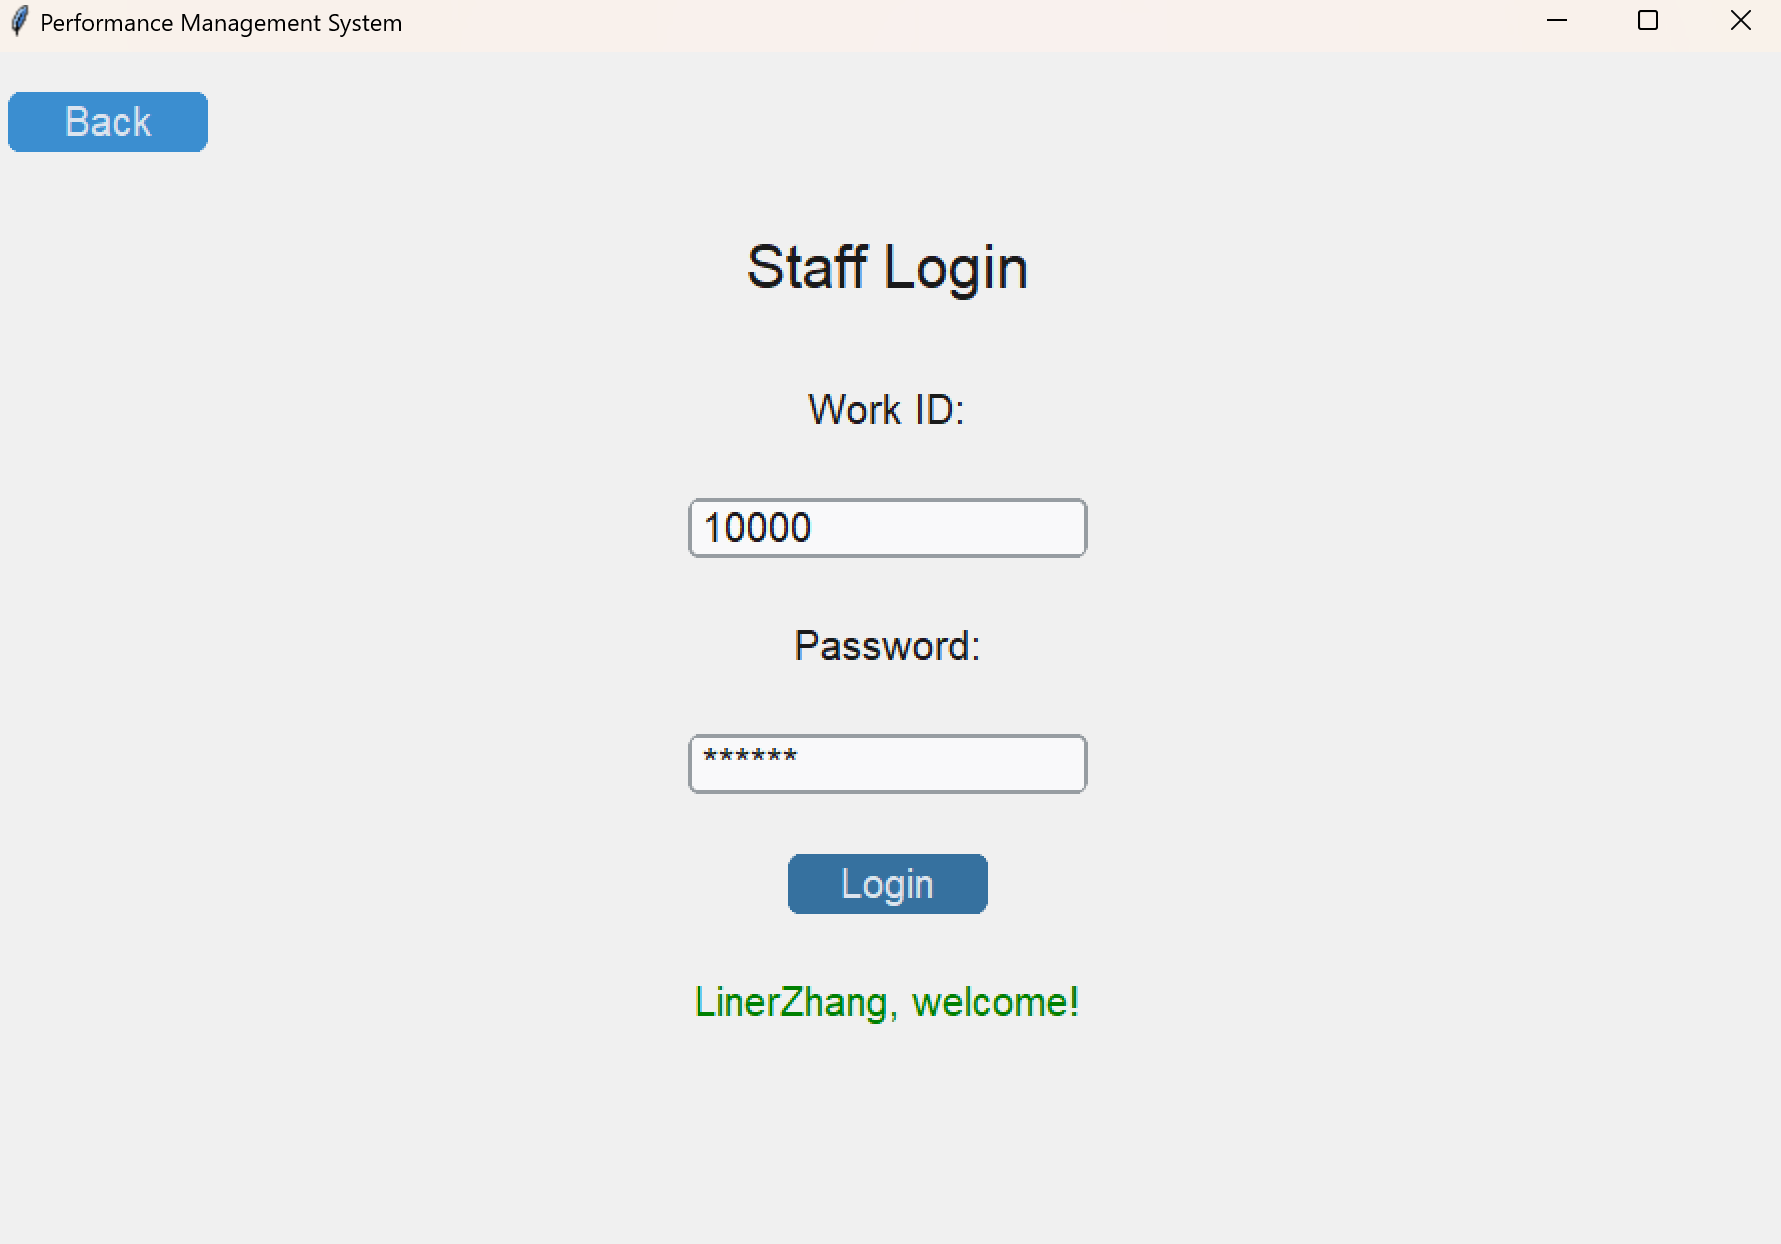
\includegraphics[width=\textwidth]{23.png}
        \caption{Staff login} 
        \label{Figure 23}
    \end{minipage}
    \hfill
    \begin{minipage}{0.48\textwidth}
        \centering
        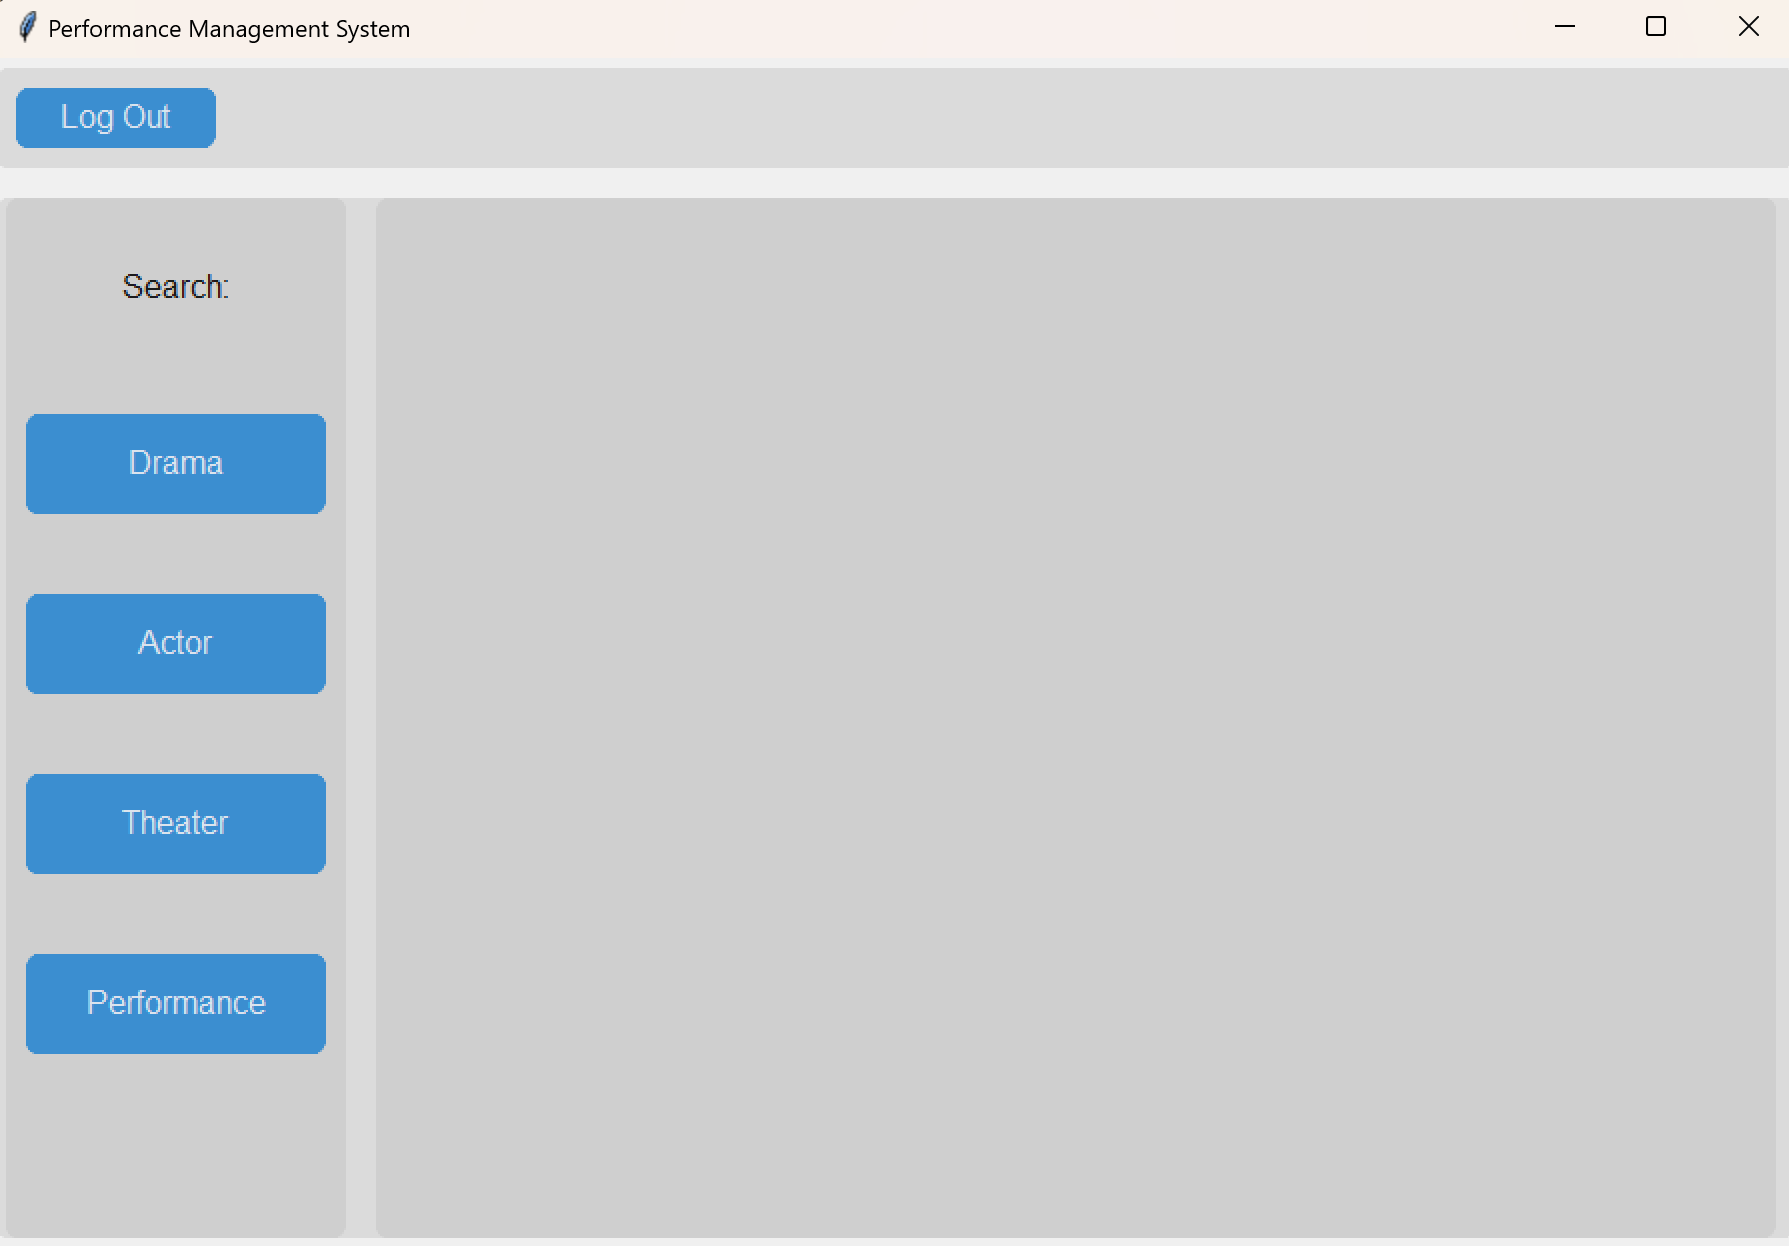
\includegraphics[width=\textwidth]{24.png}
        \caption{Staff dashboard}
        \label{Figure 24}
    \end{minipage}
\end{figure}

\subsubsection{Drama Management}
\par Clicking on 'Drama' displays all the drama information, with options to add, modify, or delete drama information using the corresponding buttons.\(Figure25-30\)
\begin{figure}[H]
    \centering
    \begin{minipage}{0.48\textwidth}
        \centering
        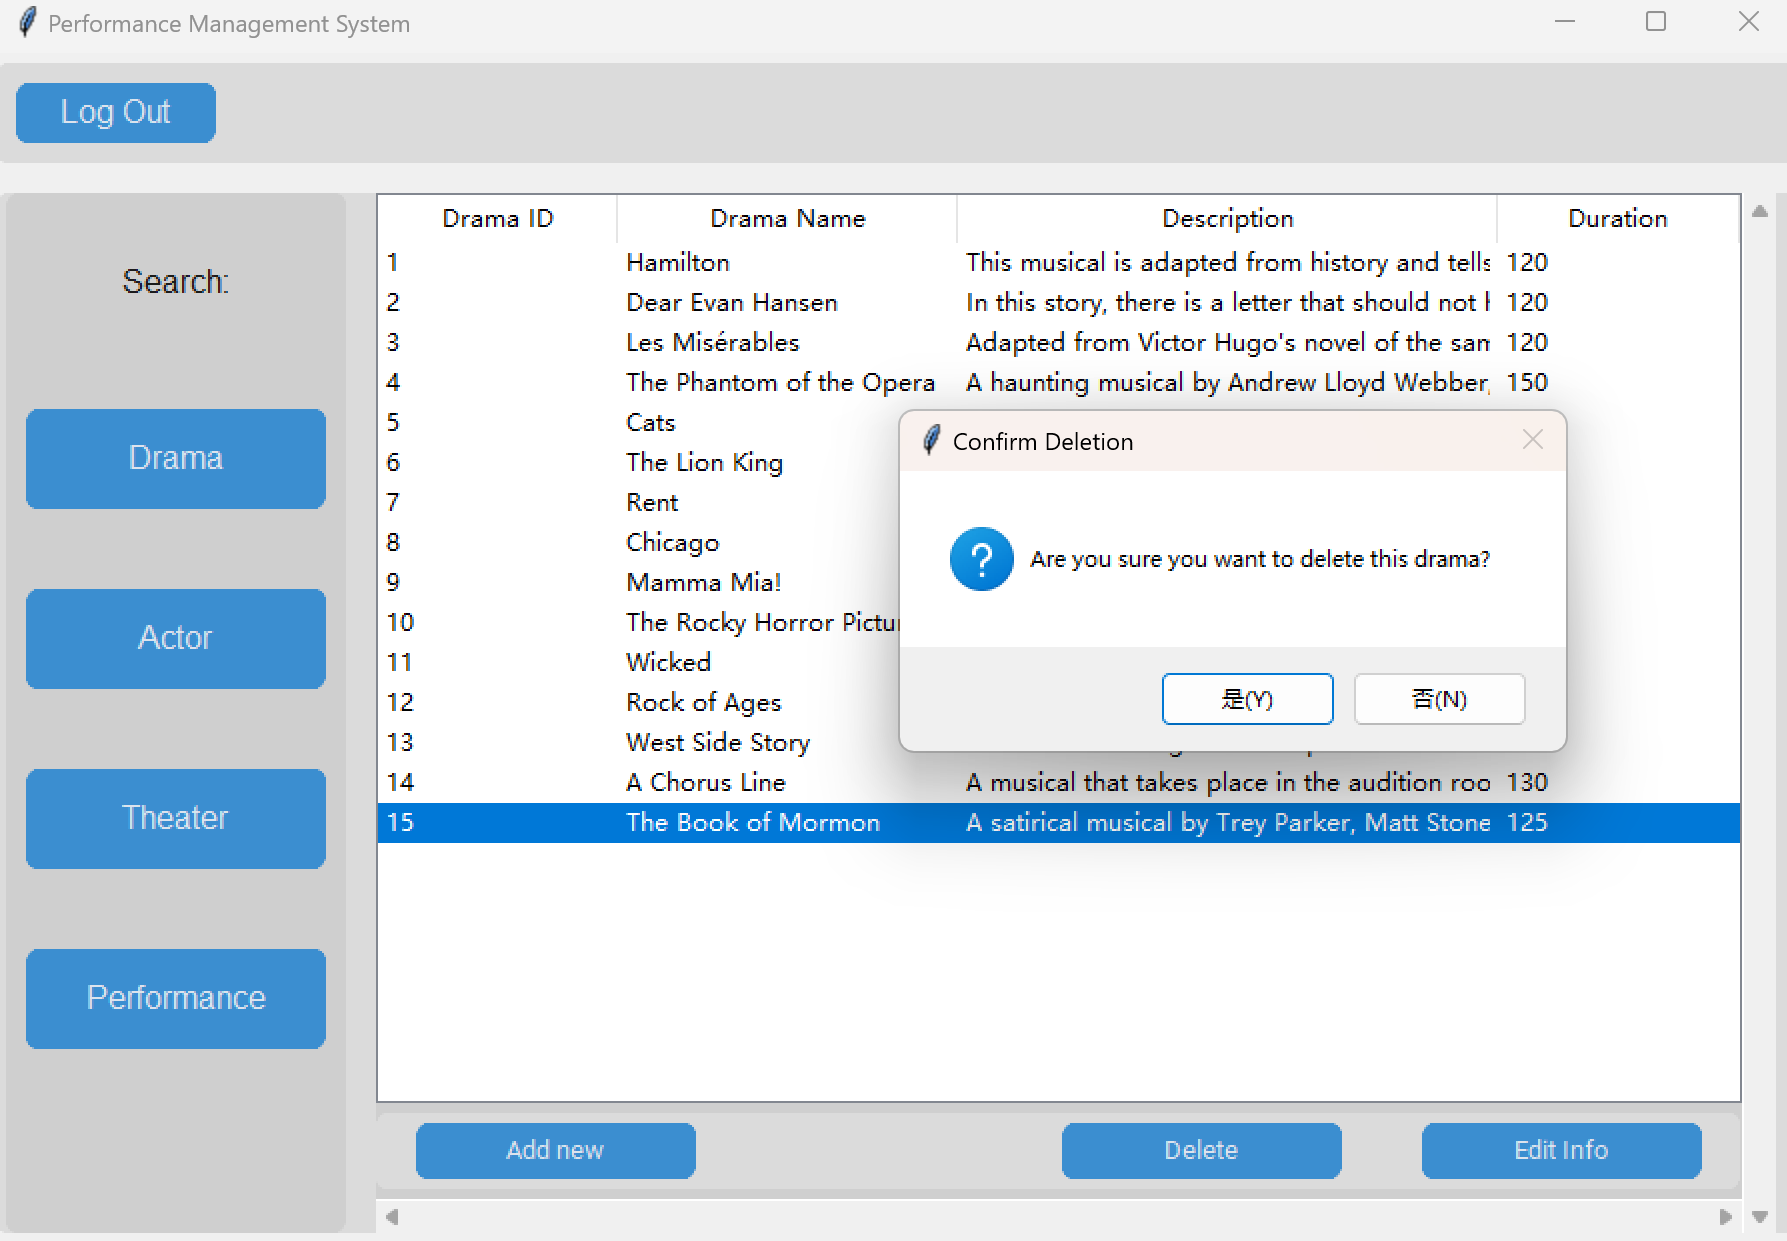
\includegraphics[width=\textwidth]{25.png}
        \caption{Drama delete} 
        \label{Figure 25}
    \end{minipage}
    \hfill
    \begin{minipage}{0.48\textwidth}
        \centering
        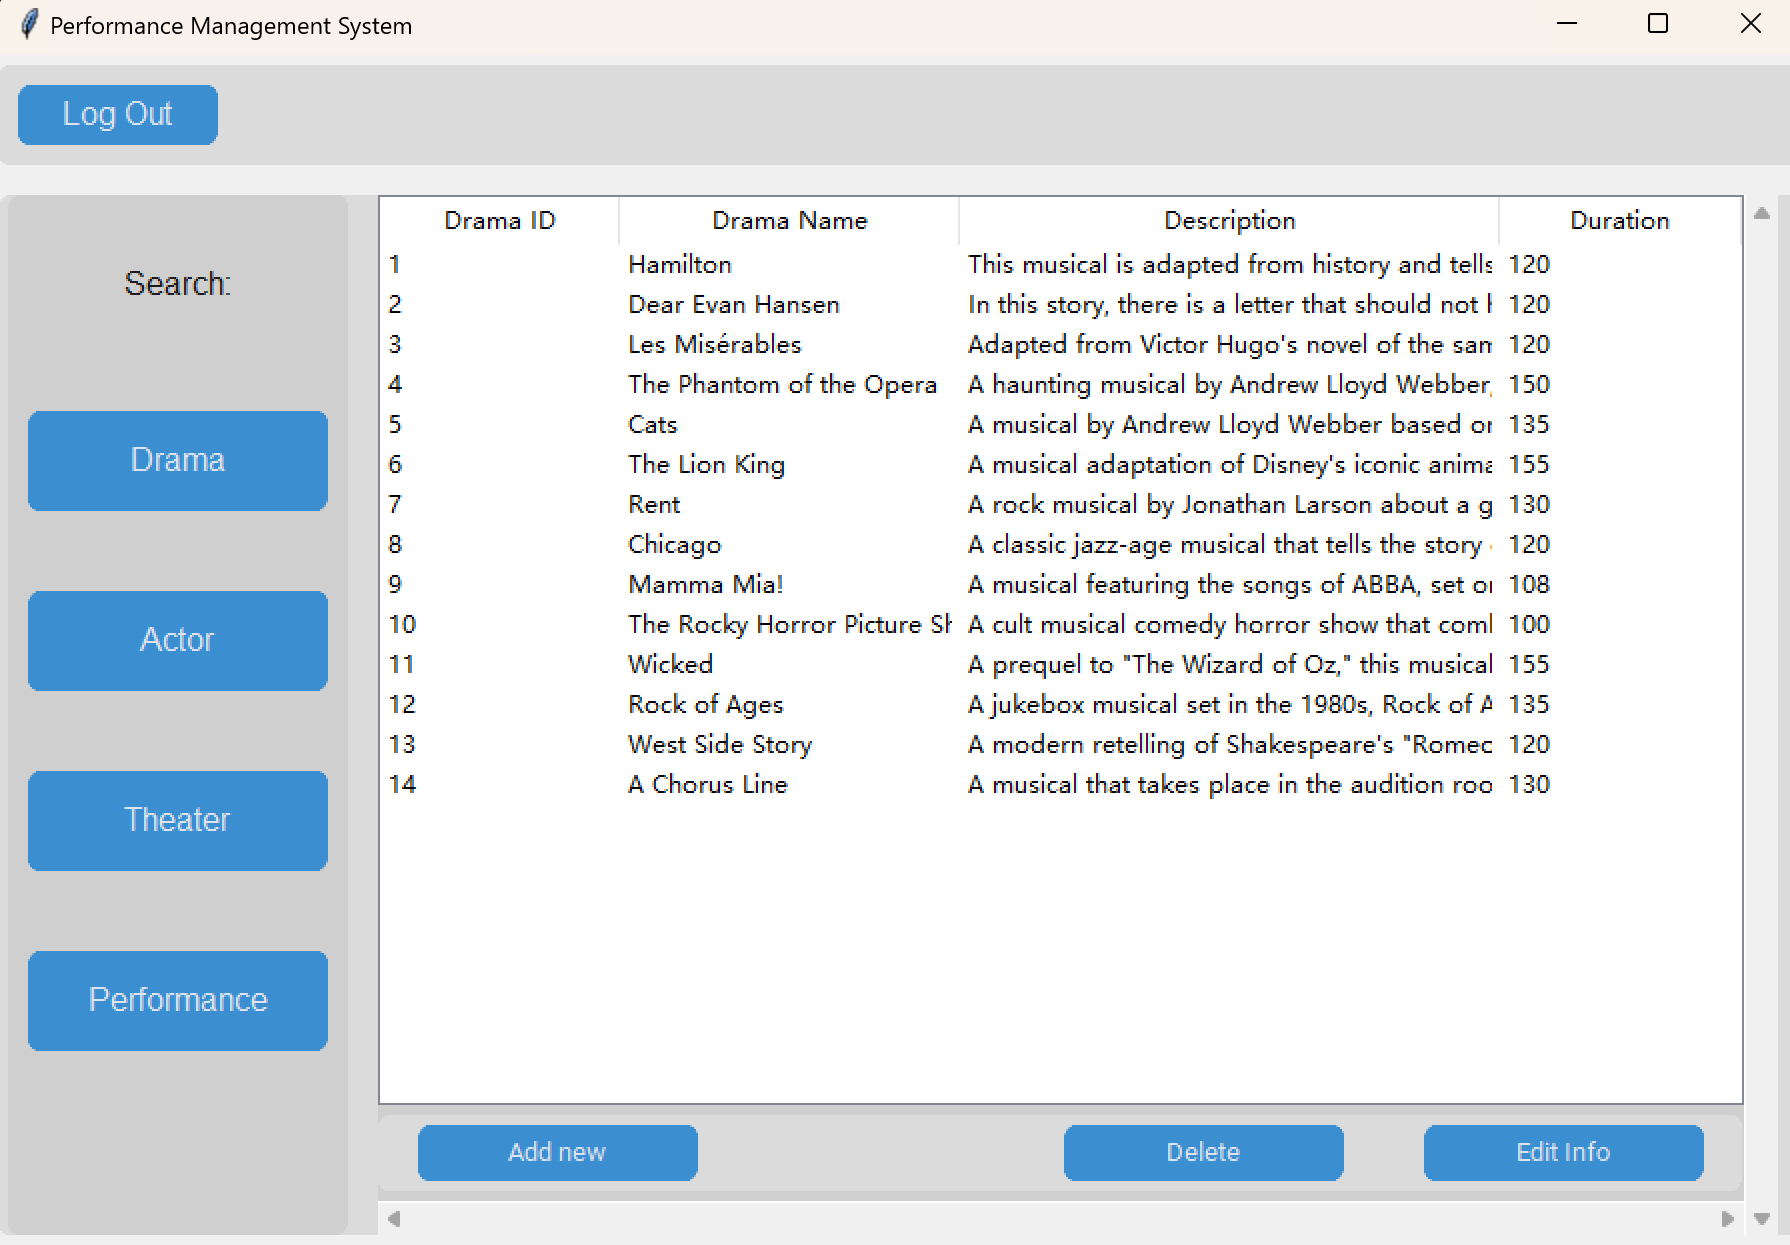
\includegraphics[width=\textwidth]{26.png}
        \caption{After deletion}
        \label{Figure 26}
    \end{minipage}
\end{figure}

\begin{figure}[H]
    \centering
    \begin{minipage}{0.48\textwidth}
        \centering
        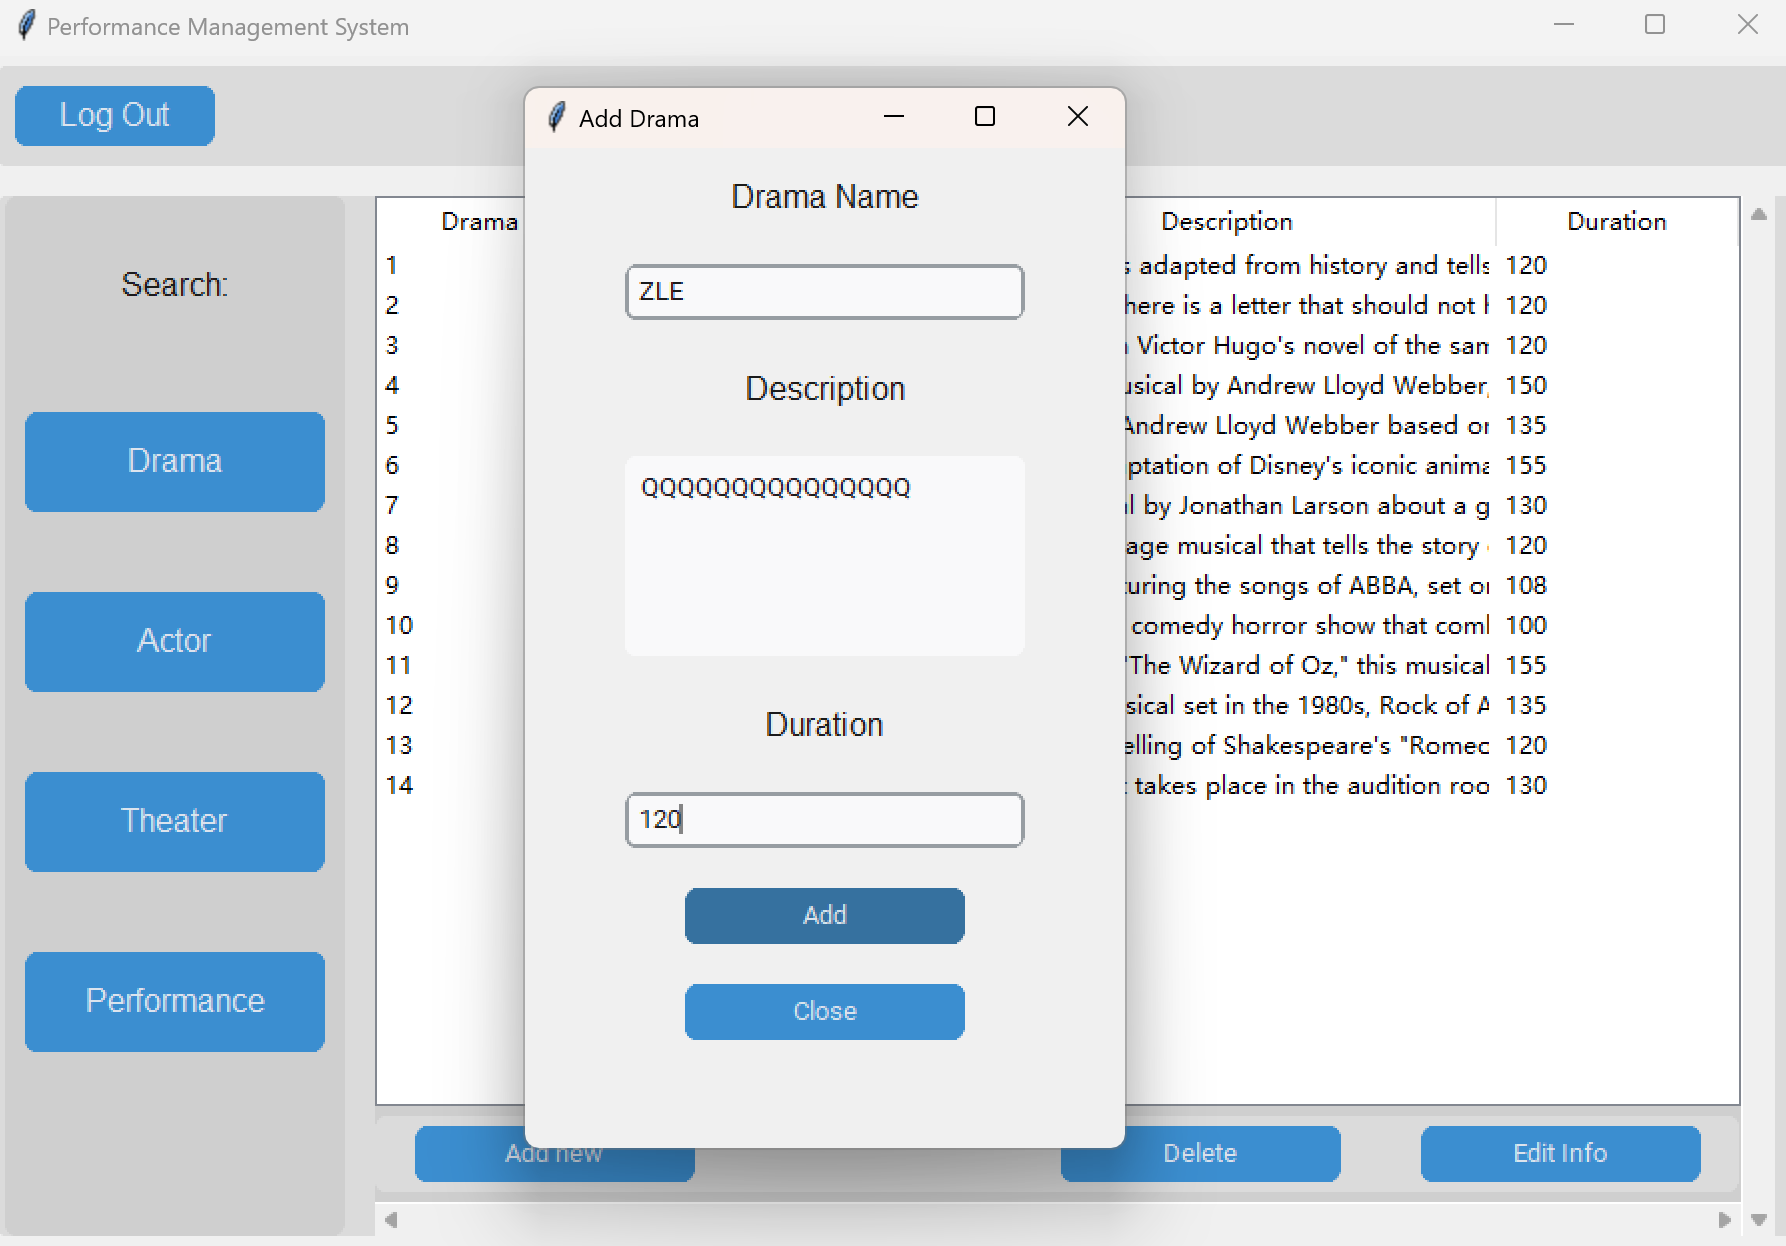
\includegraphics[width=\textwidth]{27.png}
        \caption{Drama add} 
        \label{Figure 27}
    \end{minipage}
    \hfill
    \begin{minipage}{0.48\textwidth}
        \centering
        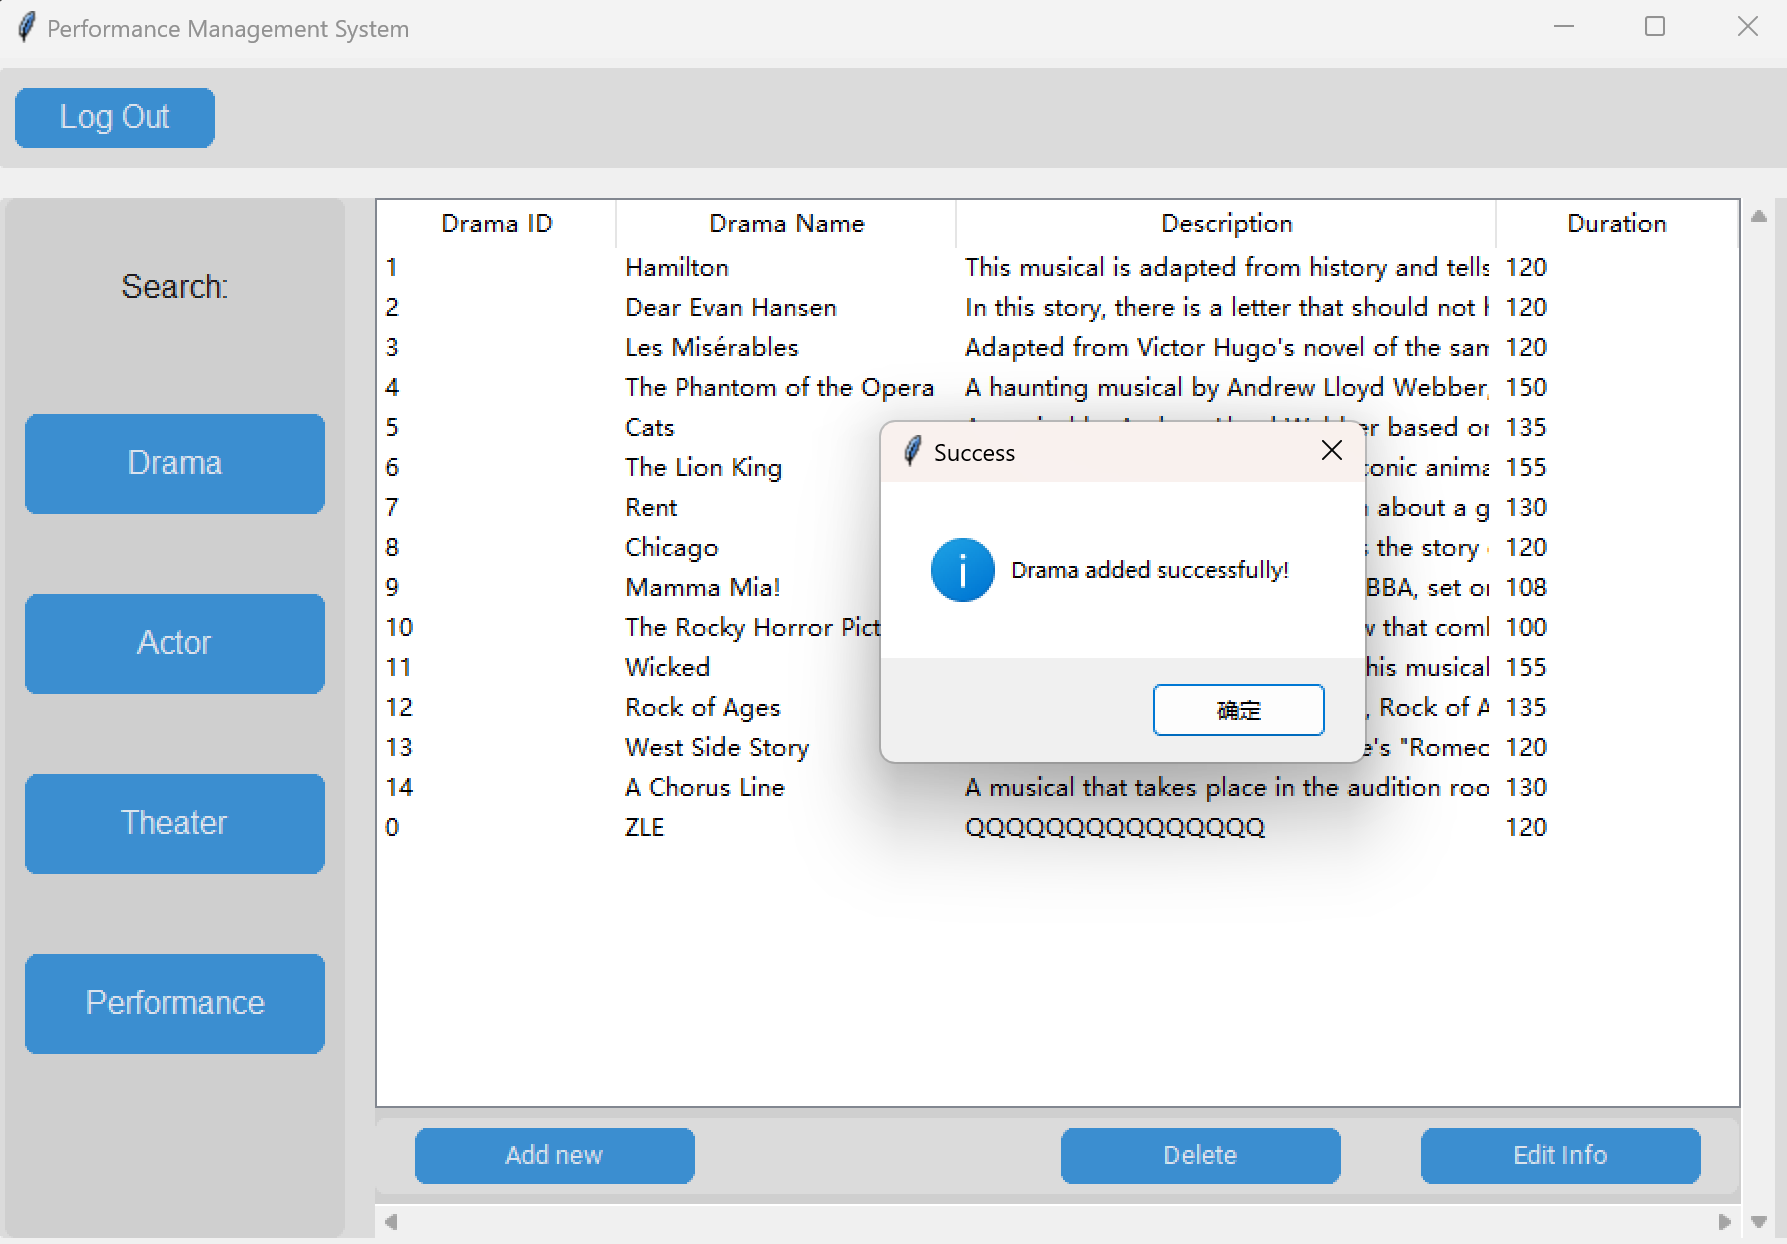
\includegraphics[width=\textwidth]{28.png}
        \caption{After add}
        \label{Figure 28}
    \end{minipage}
\end{figure}

\begin{figure}[H]
    \centering
    \begin{minipage}{0.48\textwidth}
        \centering
        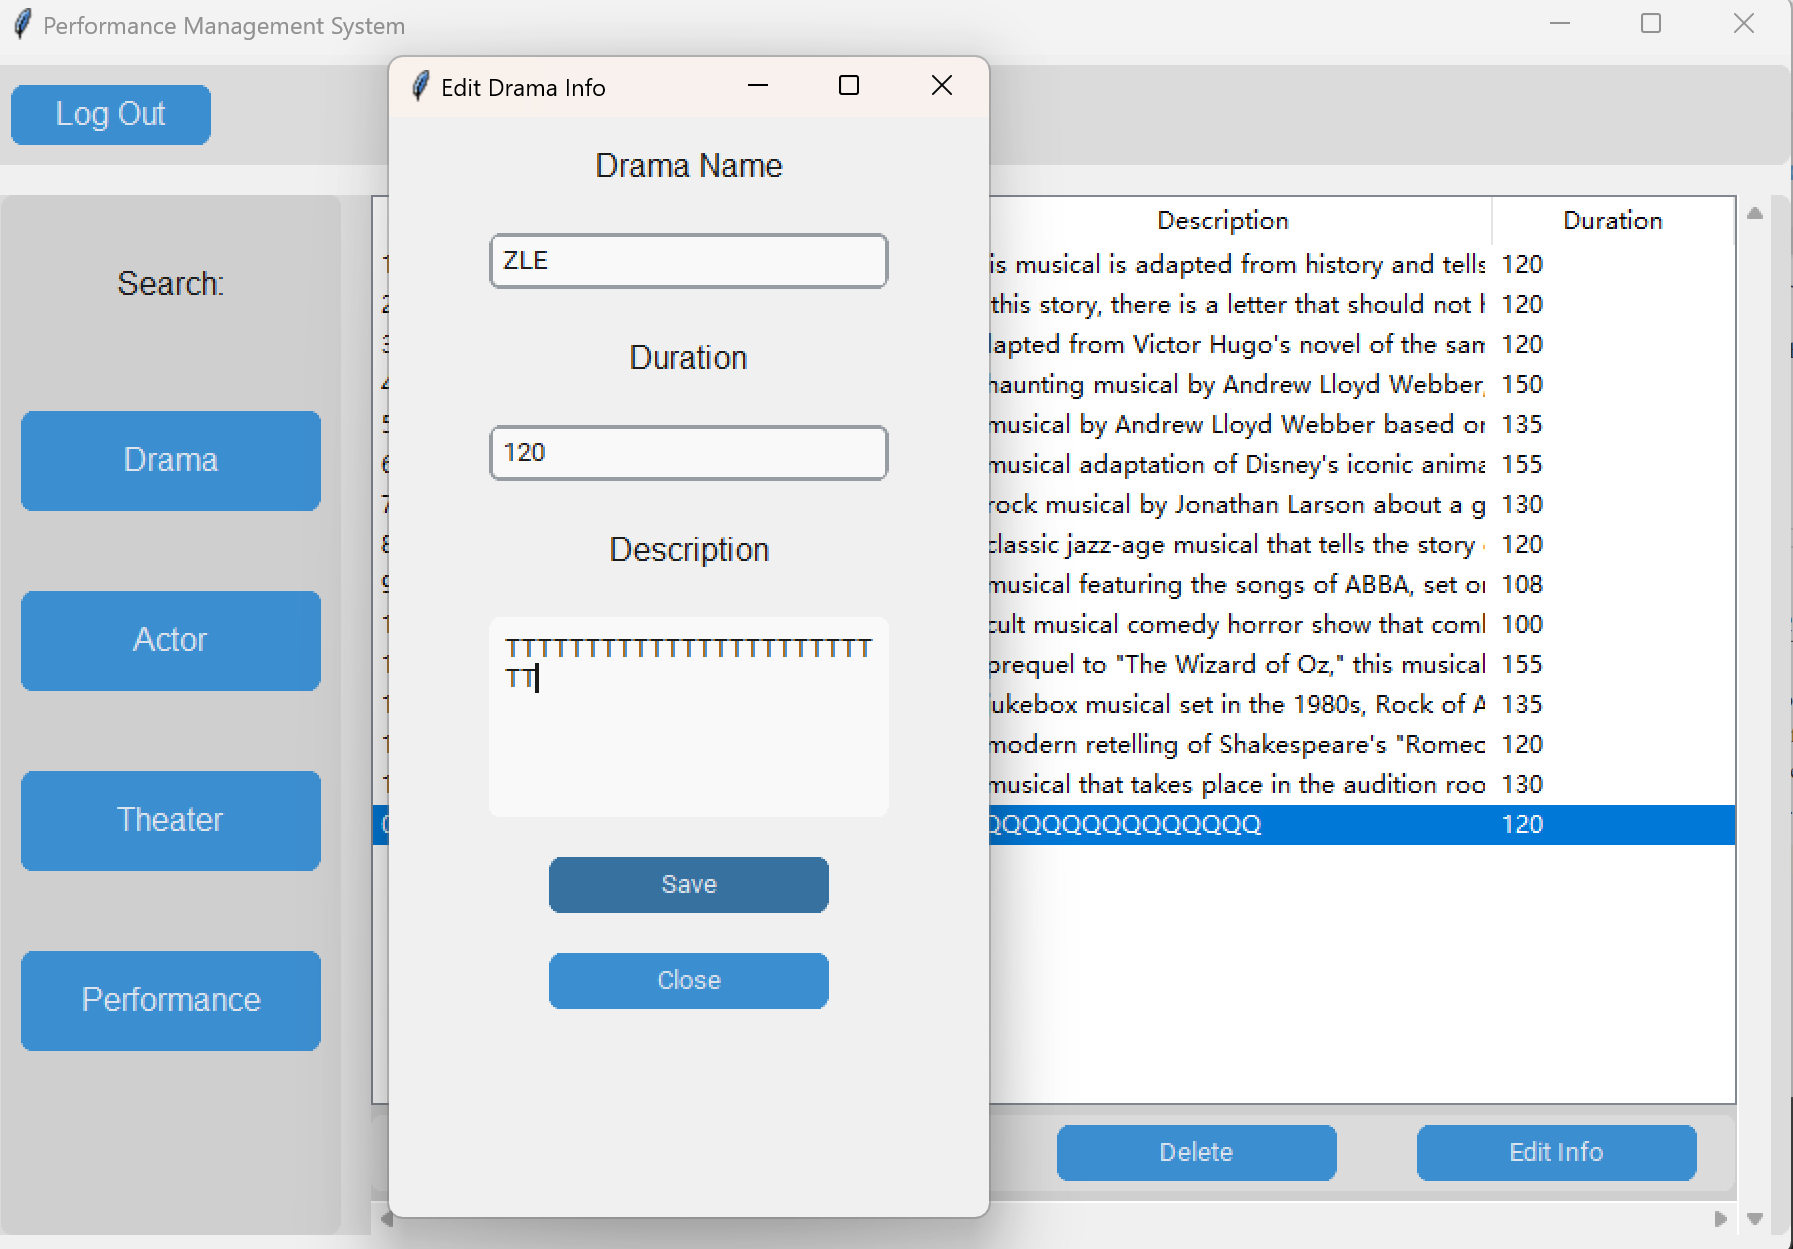
\includegraphics[width=\textwidth]{29.png}
        \caption{Drama edit} 
        \label{Figure 29}
    \end{minipage}
    \hfill
    \begin{minipage}{0.48\textwidth}
        \centering
        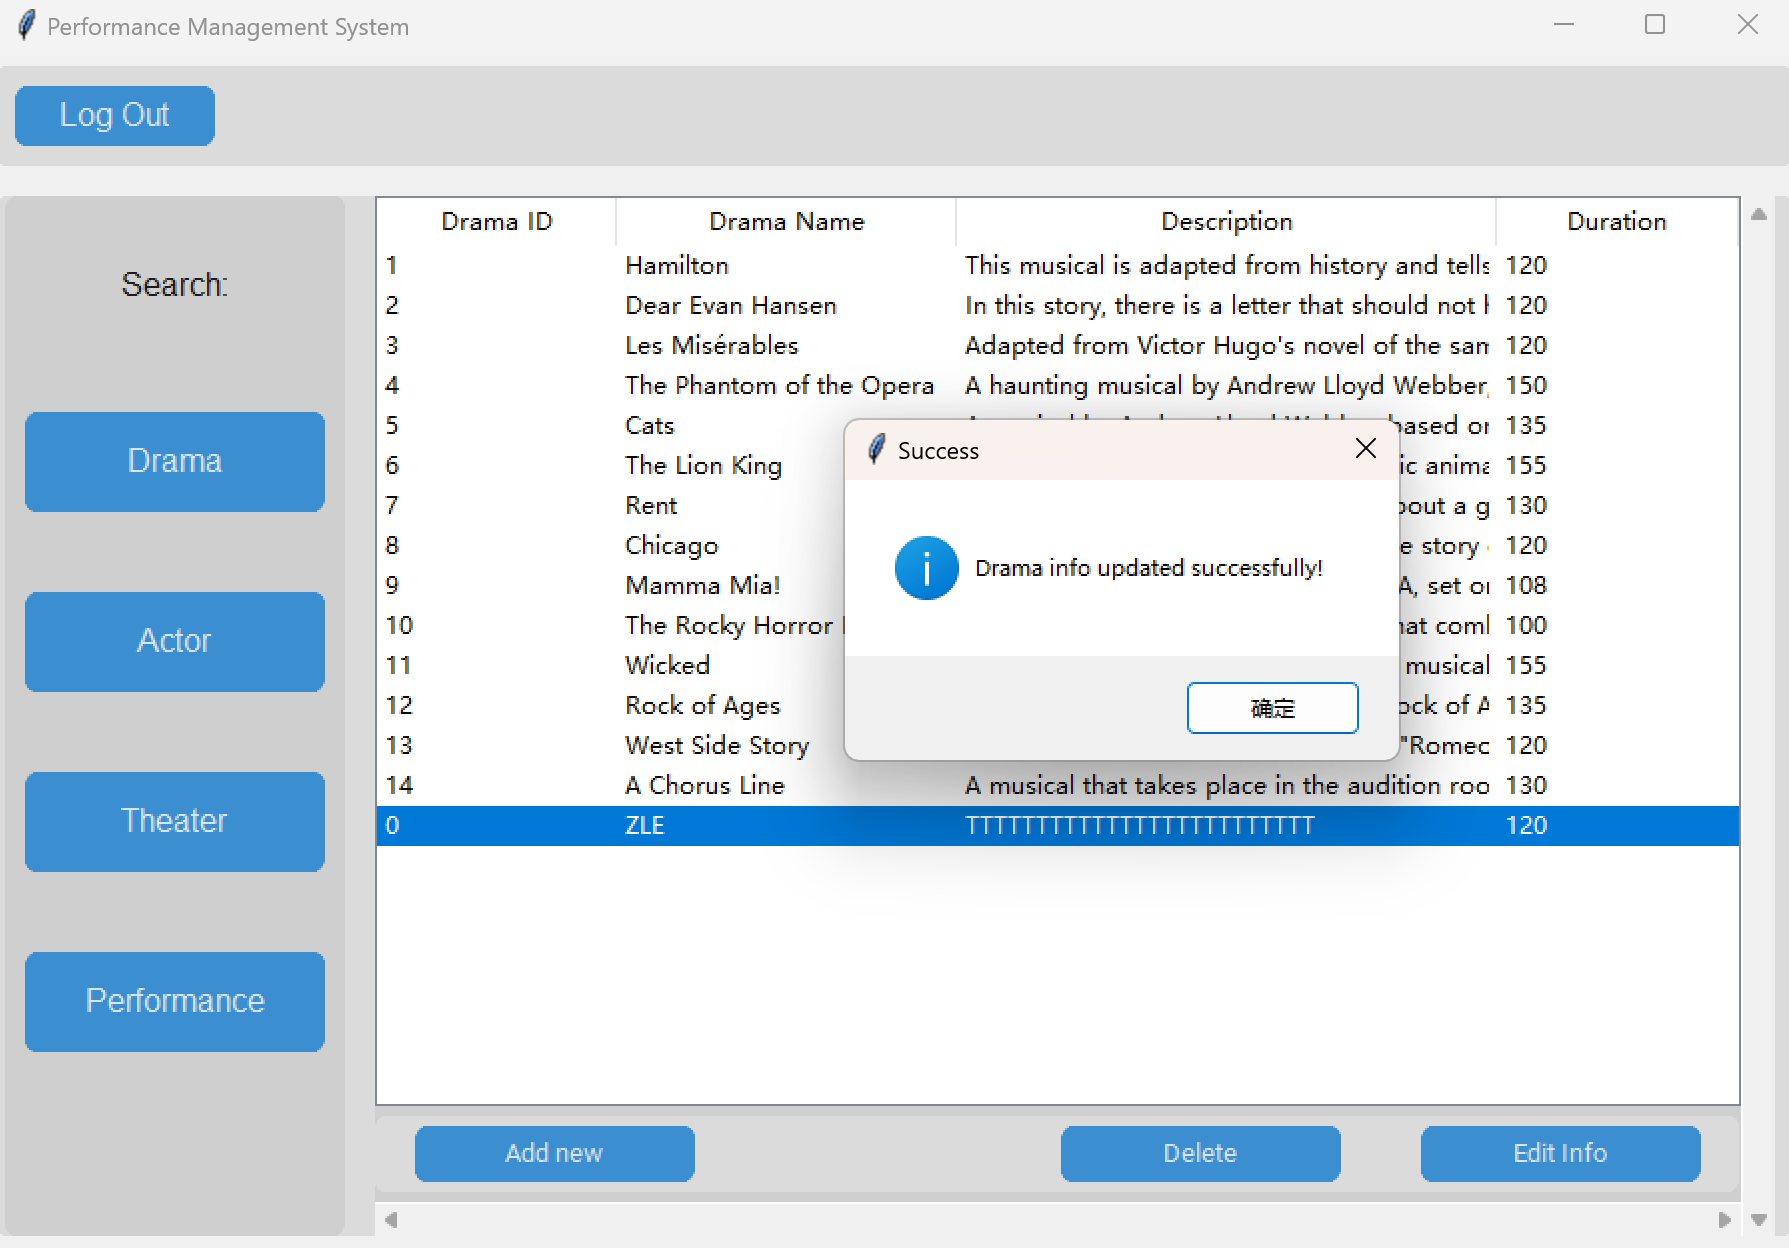
\includegraphics[width=\textwidth]{30.png}
        \caption{After edit}
        \label{Figure 30}
    \end{minipage}
\end{figure}

\subsubsection{Actor Management}
\par Clicking on 'Actor' displays all the actor information, with options to add, modify, or delete actor information using the corresponding buttons.\(Figure31-36\)
\begin{figure}[H]
    \centering
    \begin{minipage}{0.48\textwidth}
        \centering
        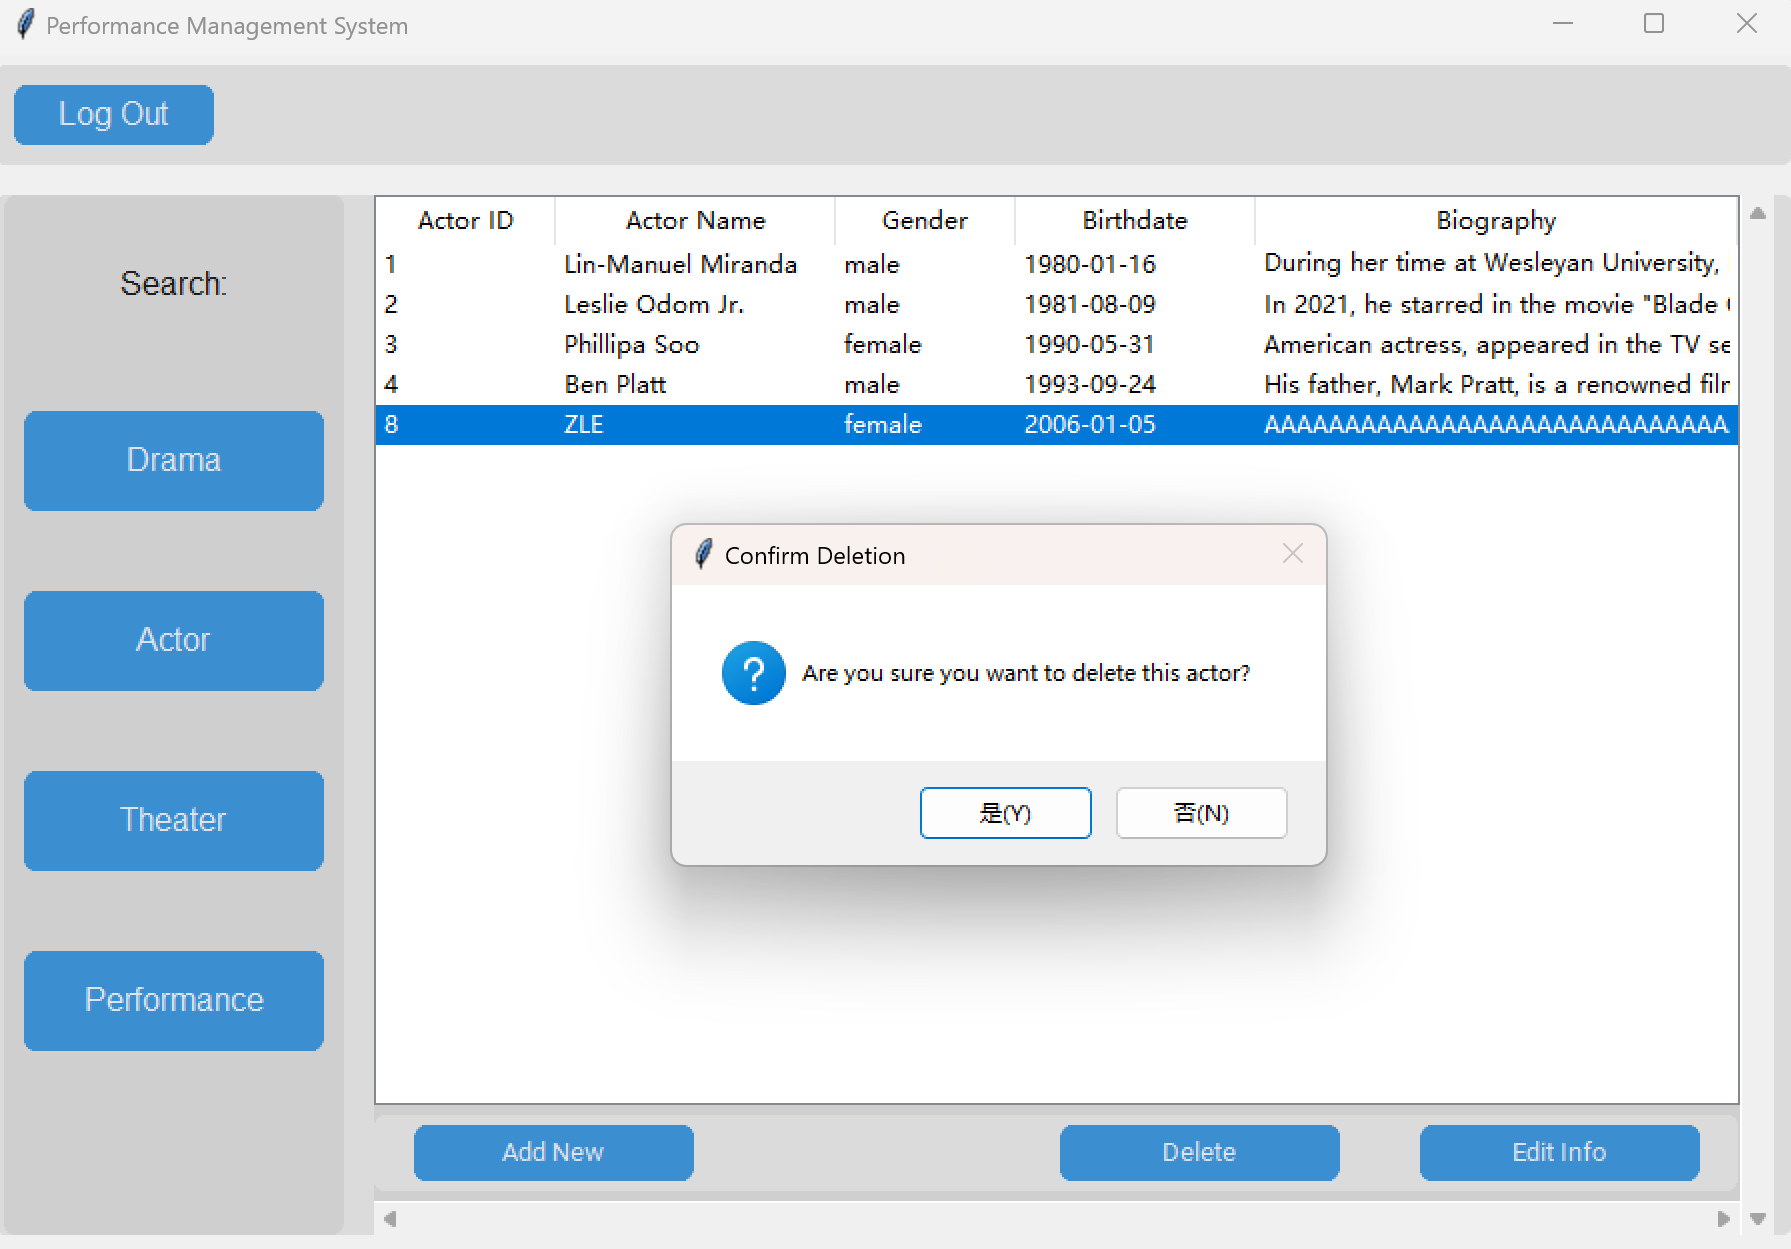
\includegraphics[width=\textwidth]{31.png}
        \caption{Actor delete} 
        \label{Figure 31}
    \end{minipage}
    \hfill
    \begin{minipage}{0.48\textwidth}
        \centering
        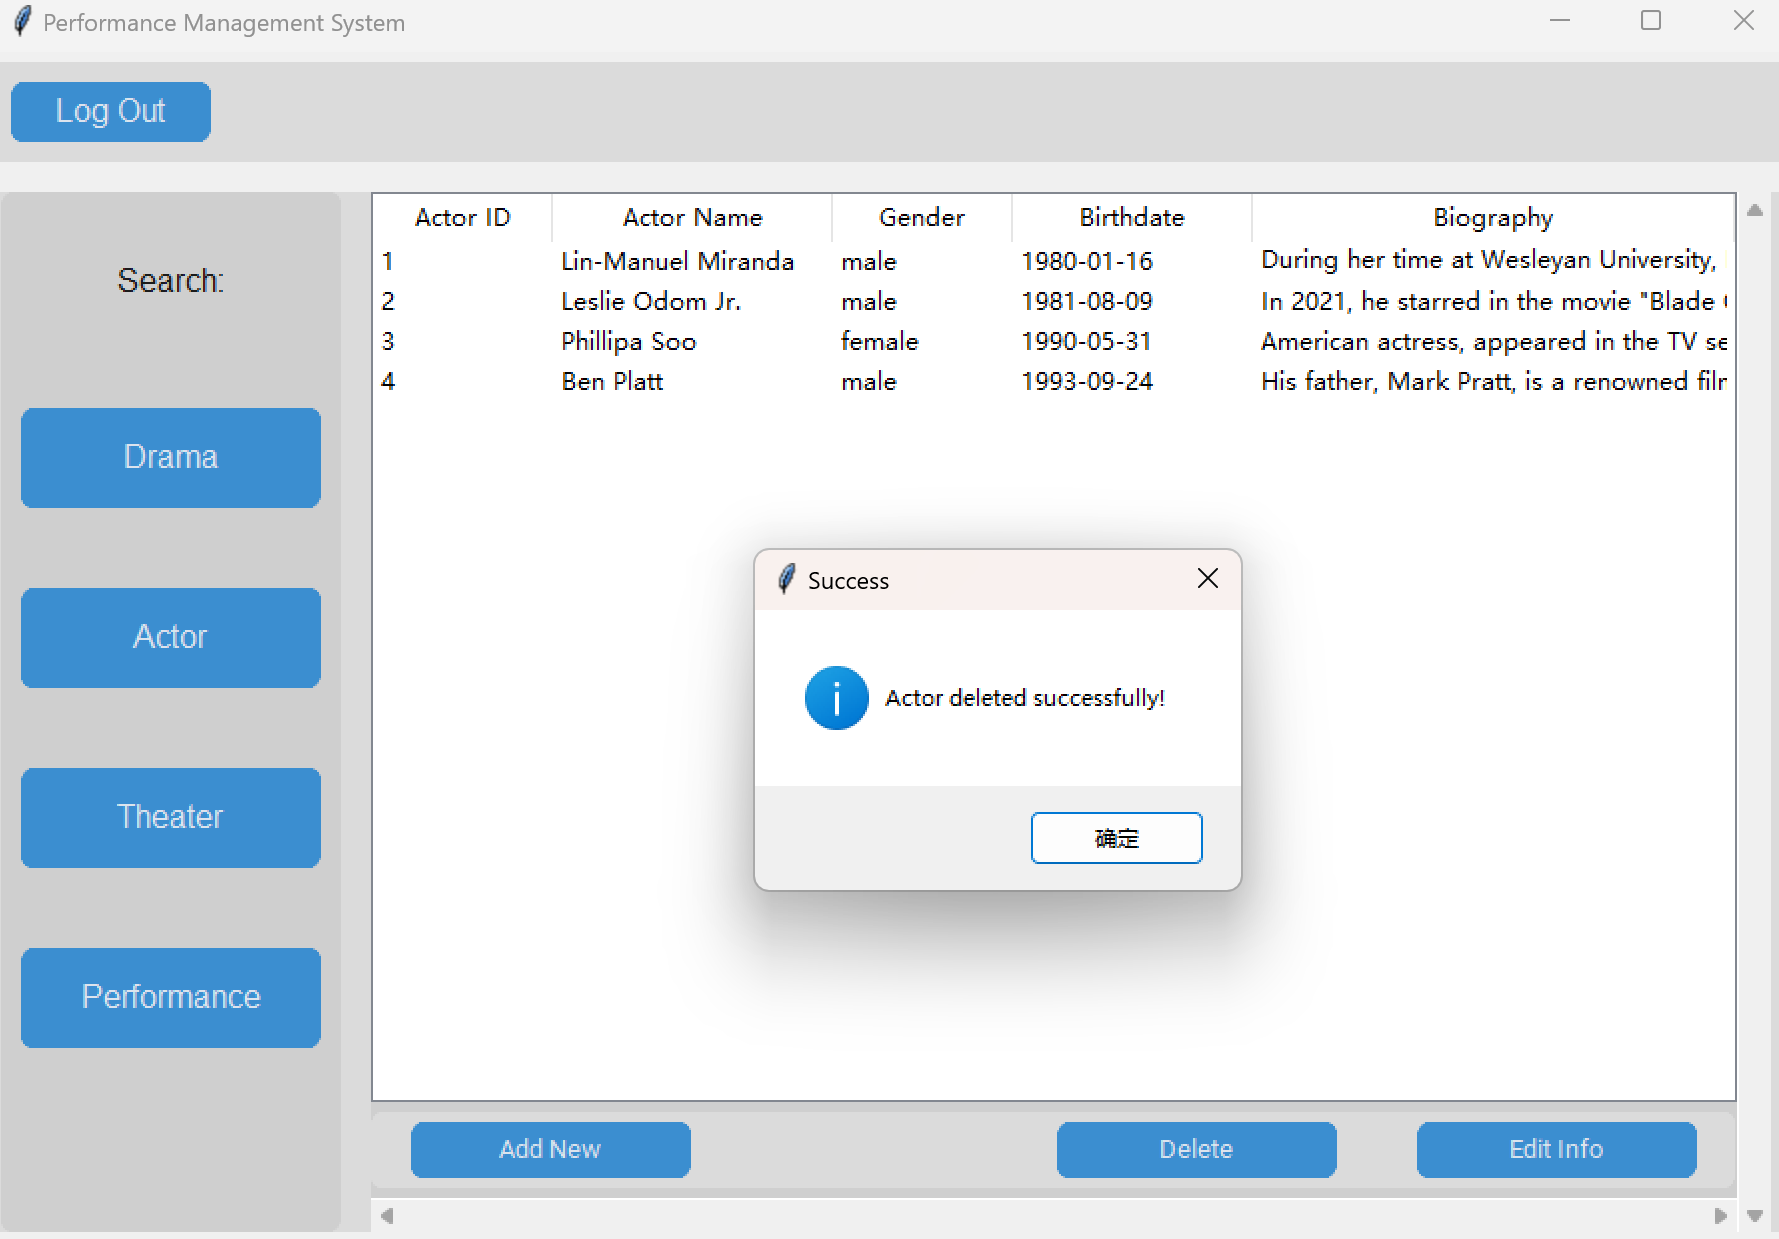
\includegraphics[width=\textwidth]{32.png}
        \caption{After deletion}
        \label{Figure 32}
    \end{minipage}
\end{figure}

\begin{figure}[H]
    \centering
    \begin{minipage}{0.48\textwidth}
        \centering
        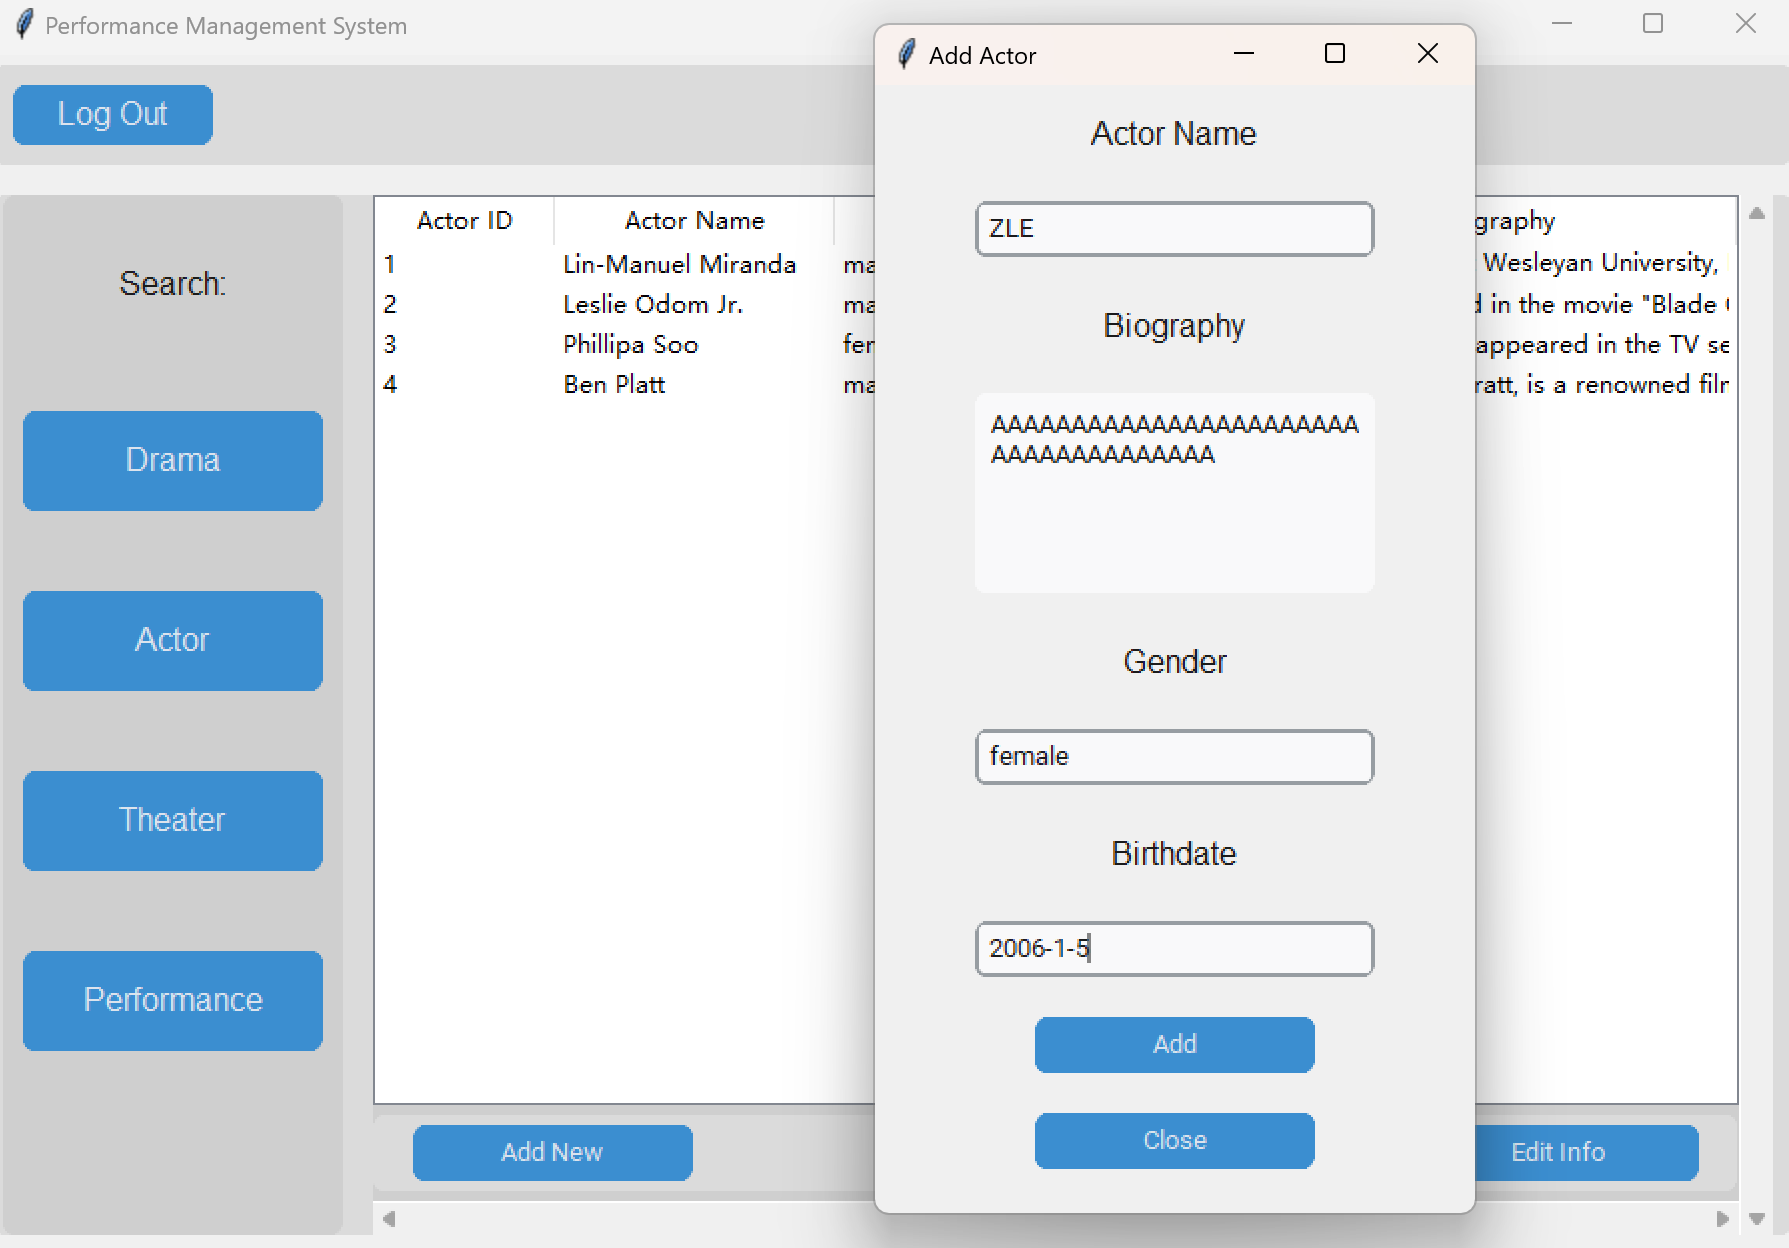
\includegraphics[width=\textwidth]{33.png}
        \caption{Actor add} 
        \label{Figure 33}
    \end{minipage}
    \hfill
    \begin{minipage}{0.48\textwidth}
        \centering
        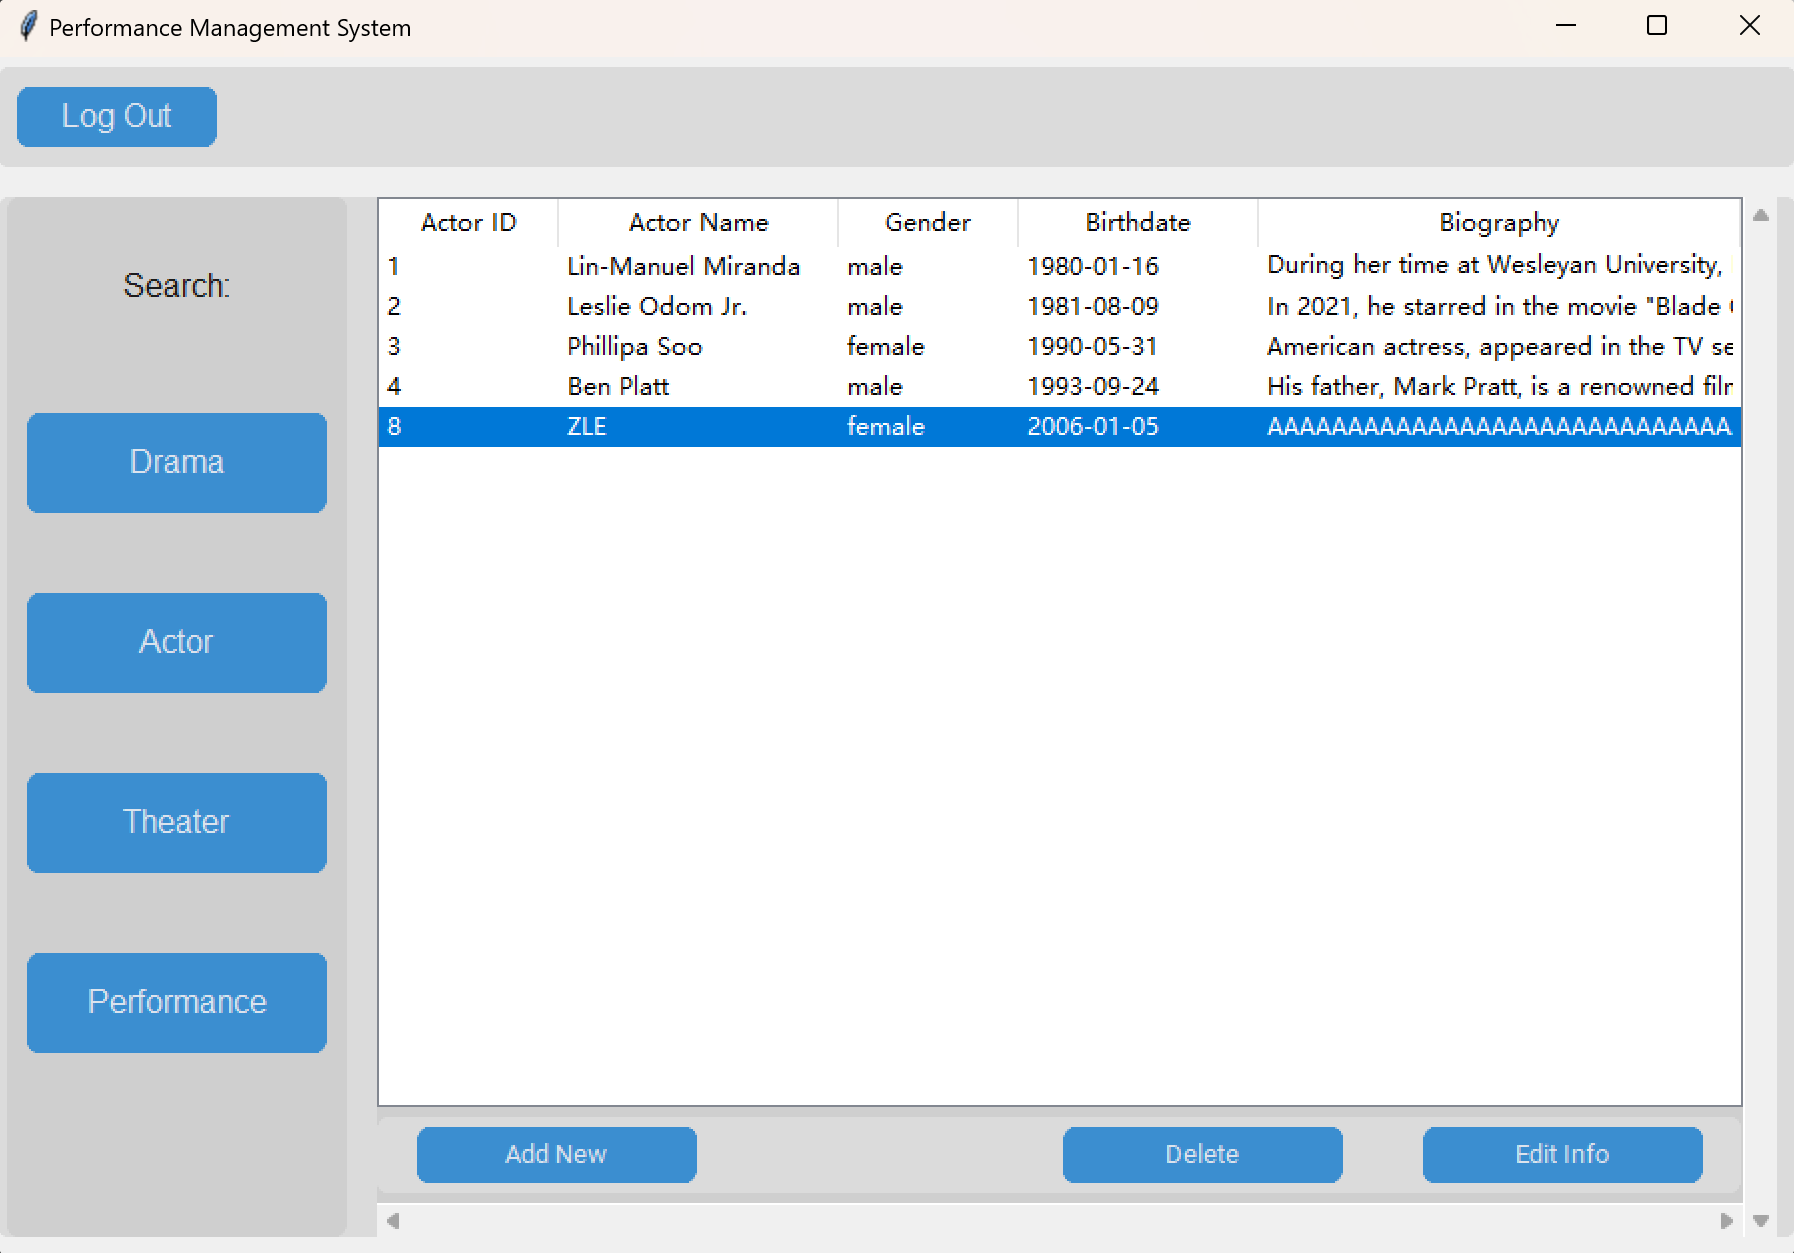
\includegraphics[width=\textwidth]{34.png}
        \caption{After add}
        \label{Figure 34}
    \end{minipage}
\end{figure}

\begin{figure}[H]
    \centering
    \begin{minipage}{0.48\textwidth}
        \centering
        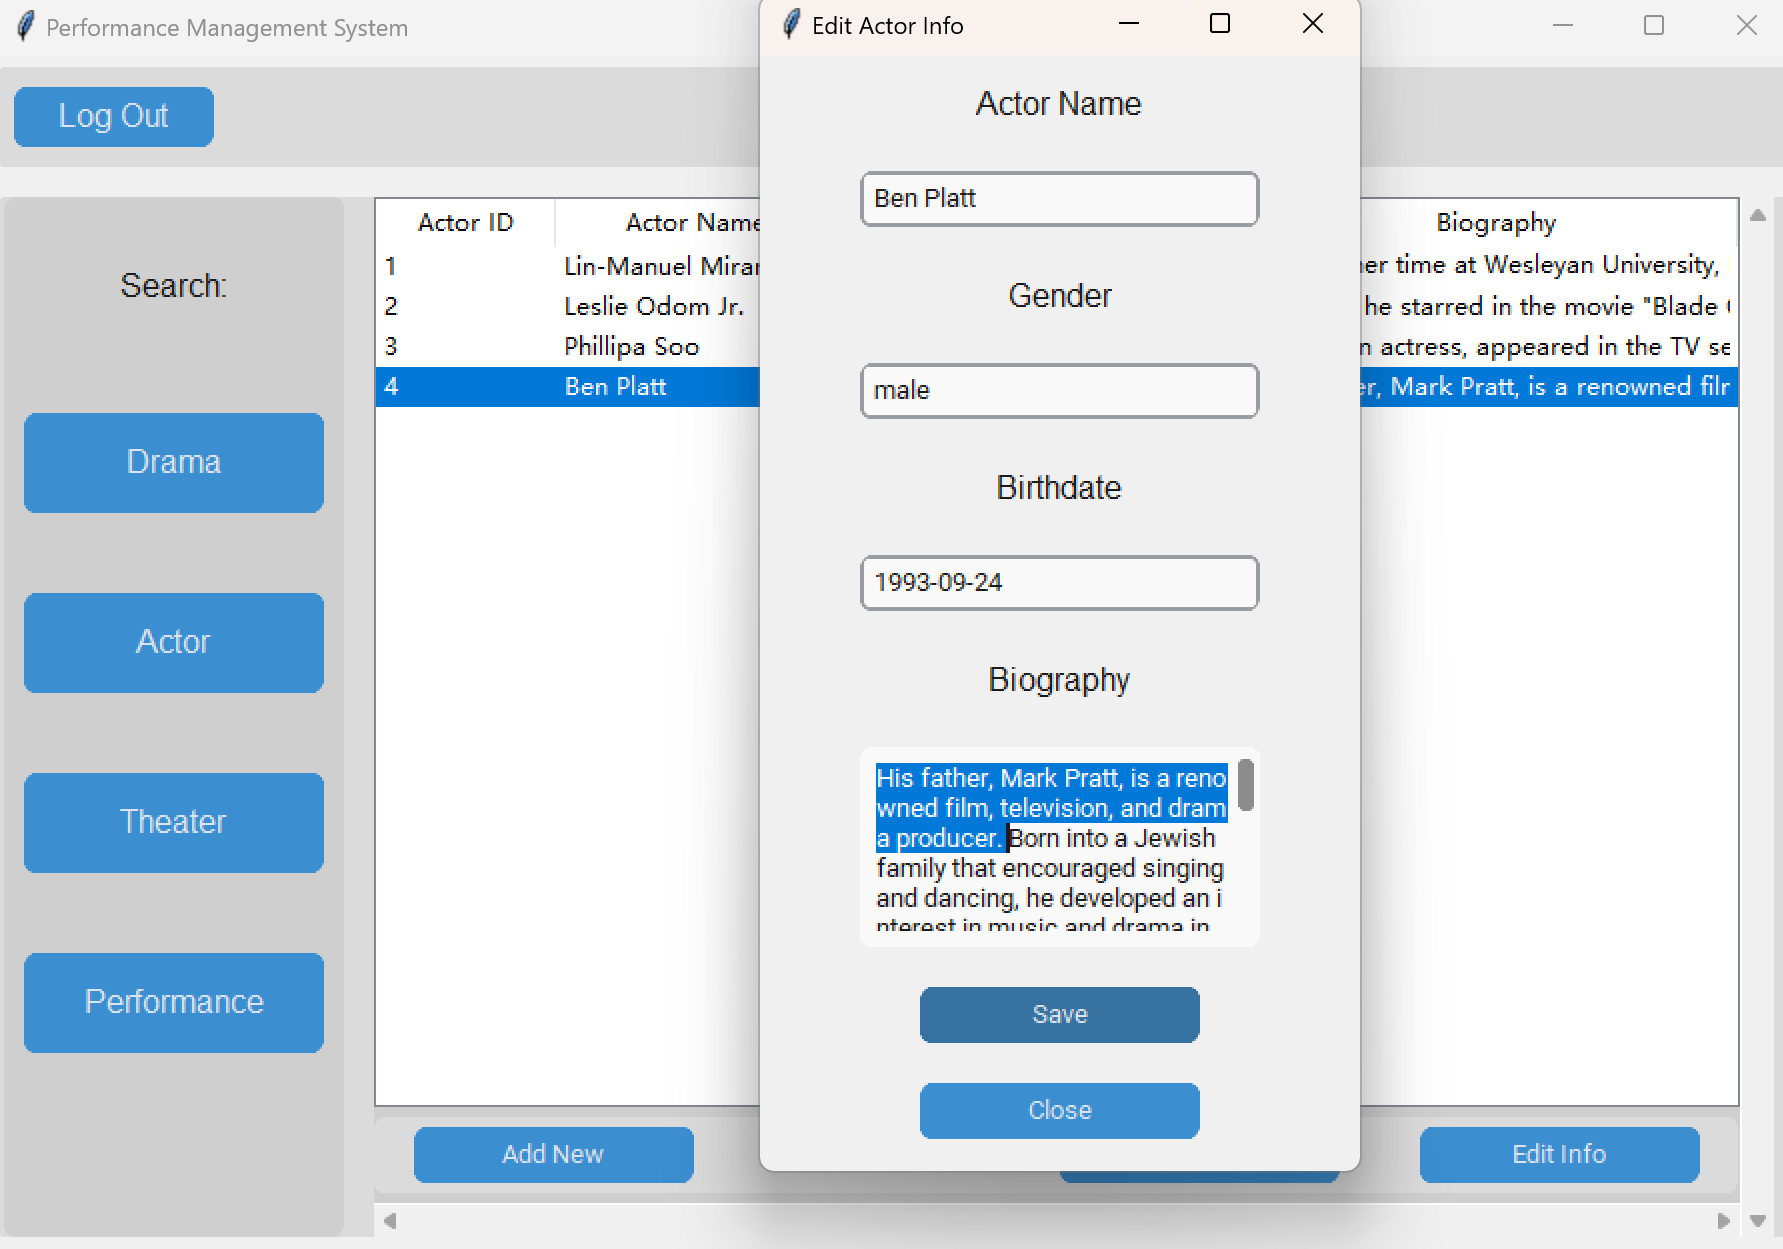
\includegraphics[width=\textwidth]{35.png}
        \caption{Actor edit} 
        \label{Figure 35}
    \end{minipage}
    \hfill
    \begin{minipage}{0.48\textwidth}
        \centering
        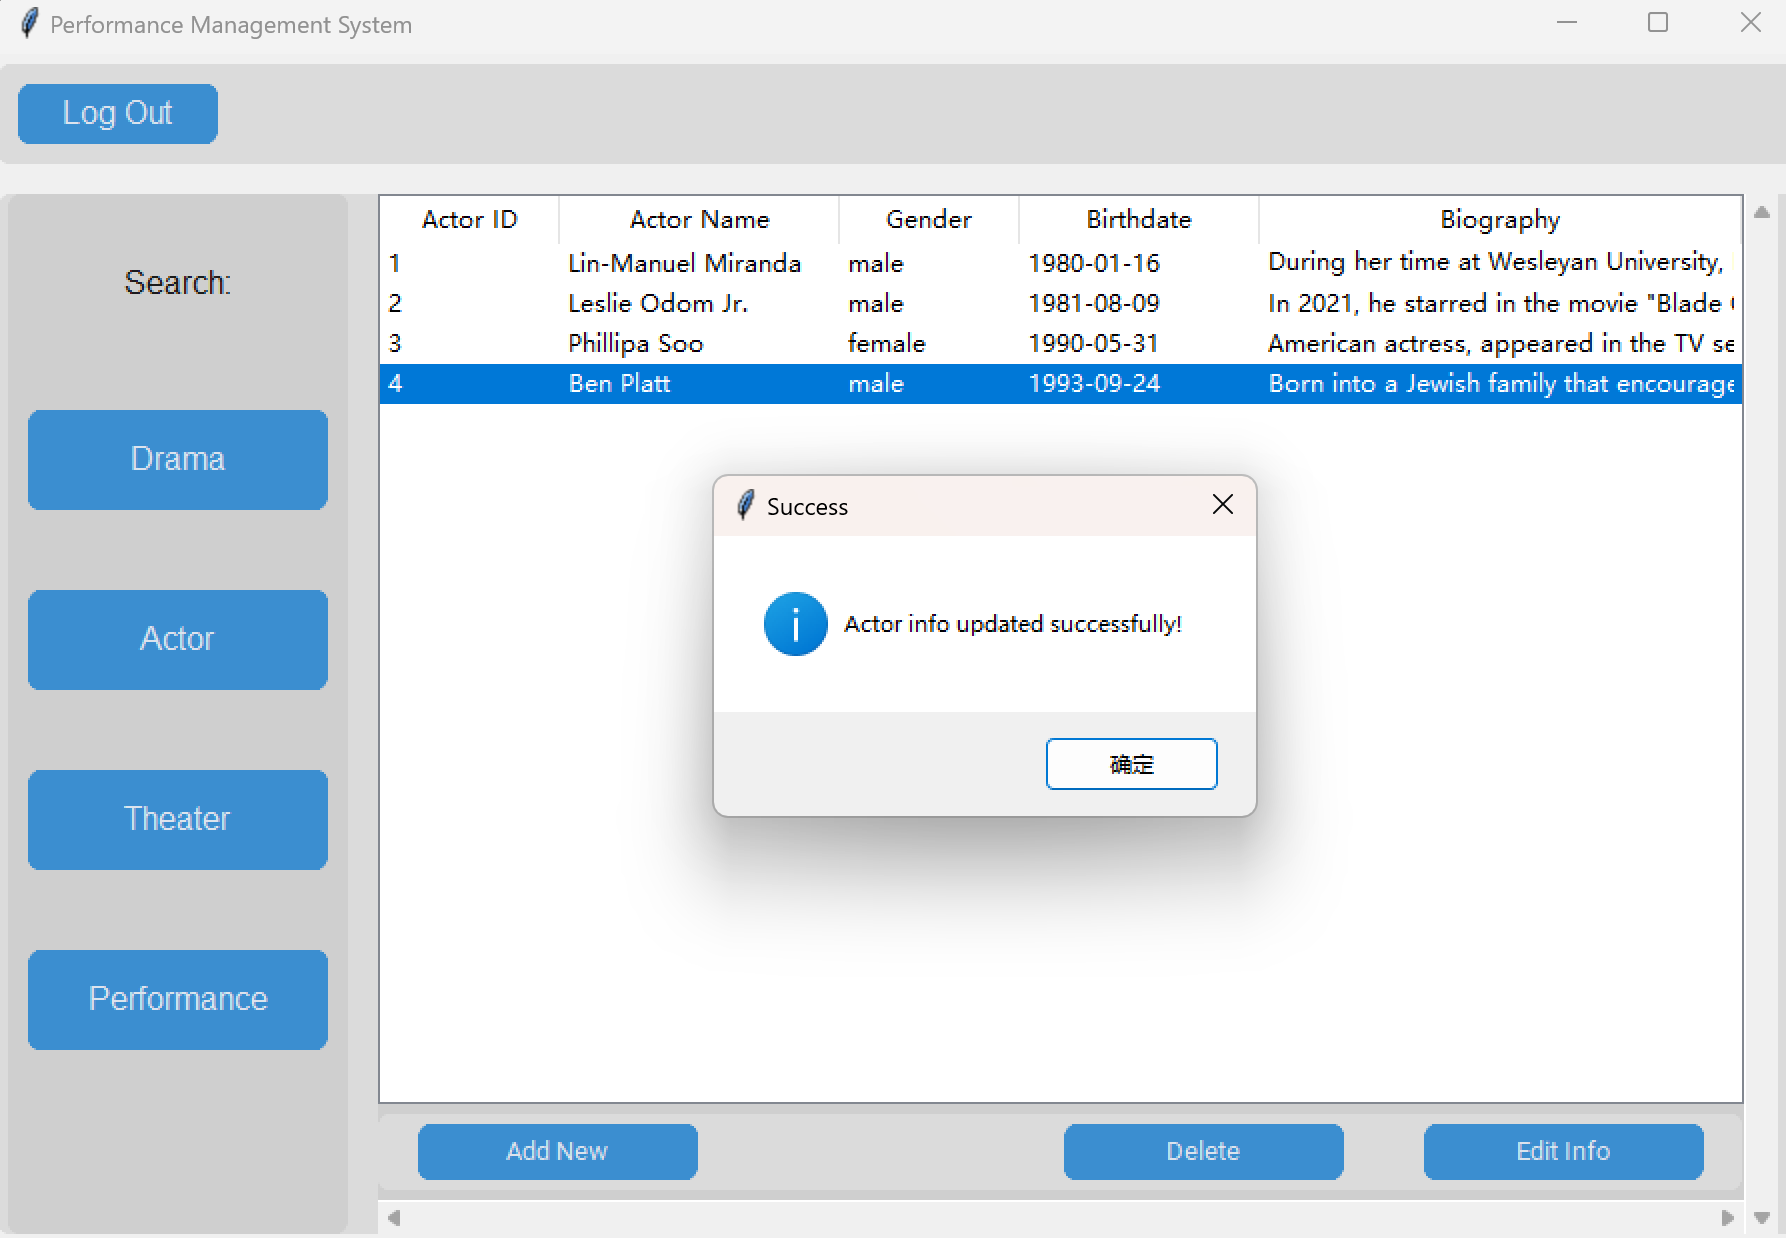
\includegraphics[width=\textwidth]{36.png}
        \caption{After edit}
        \label{Figure 36}
    \end{minipage}
\end{figure}

\subsubsection{Theater Management}
\par Clicking on 'Theater' displays all the theater information, with options to add, modify, or delete theater information using the corresponding buttons.\(Figure37-42\)
\begin{figure}[H]
    \centering
    \begin{minipage}{0.48\textwidth}
        \centering
        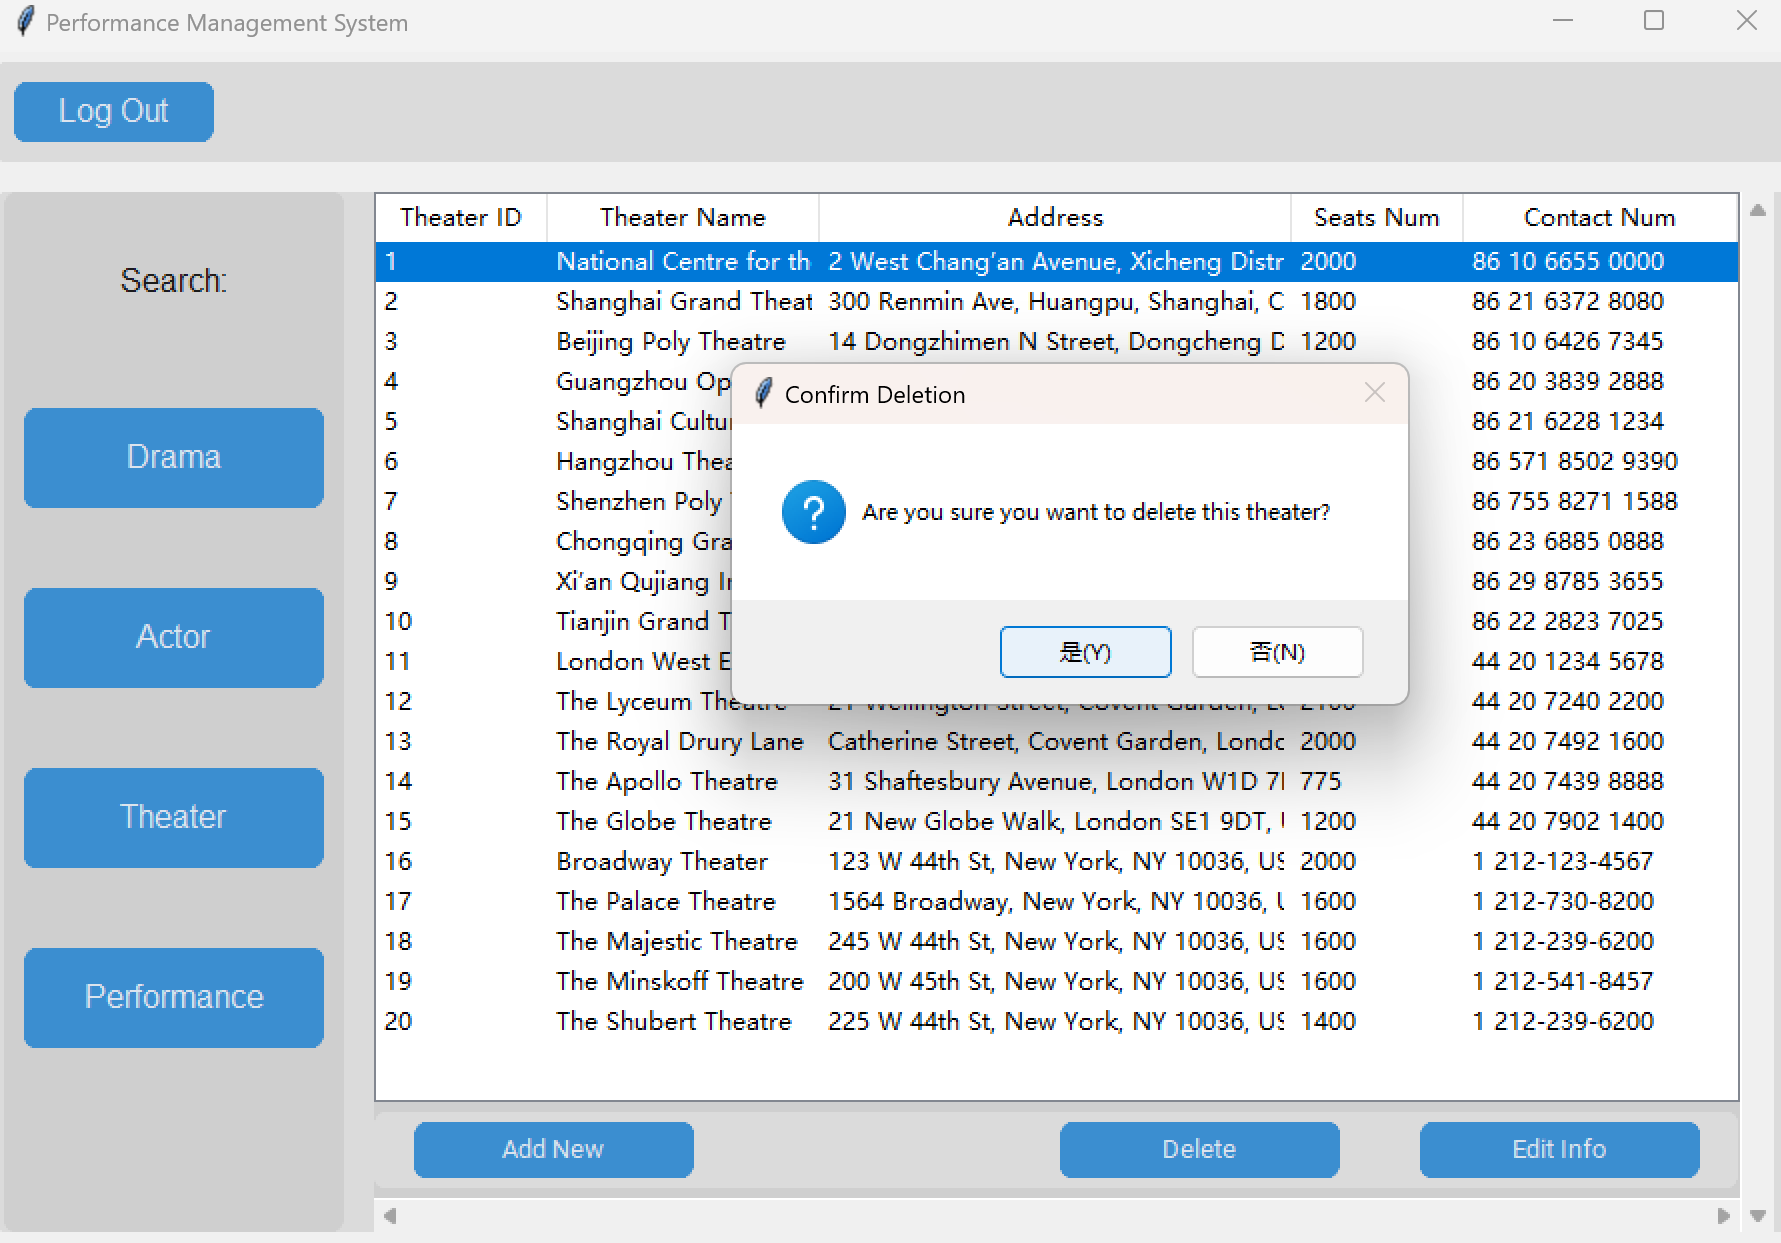
\includegraphics[width=\textwidth]{37.png}

        \caption{Theater delete} 
        \label{Figure 37}
    \end{minipage}
    \hfill
    \begin{minipage}{0.48\textwidth}
        \centering
        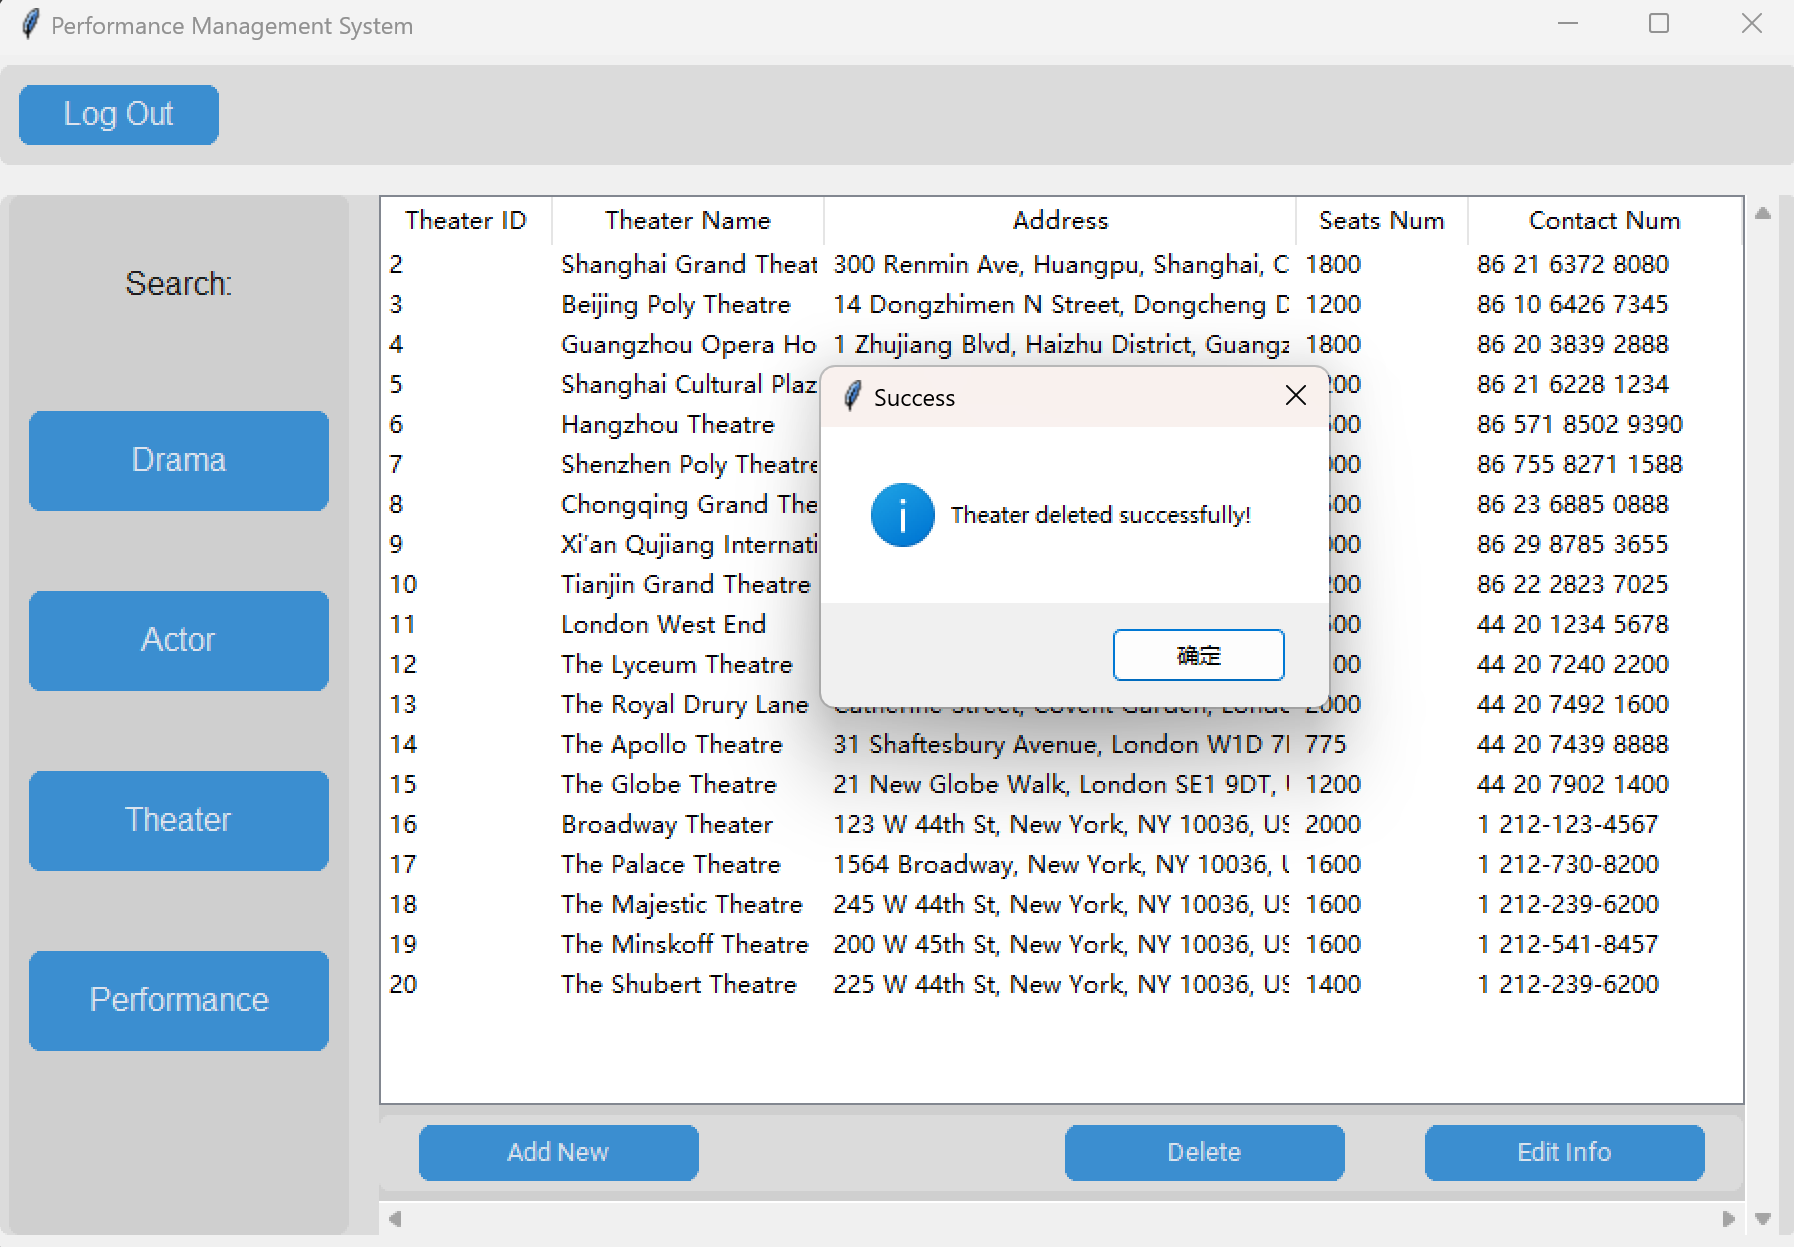
\includegraphics[width=\textwidth]{38.png}
        \caption{After deletion}
        \label{Figure 38}
    \end{minipage}
\end{figure}

\begin{figure}[H]
    \centering
    \begin{minipage}{0.48\textwidth}
        \centering
        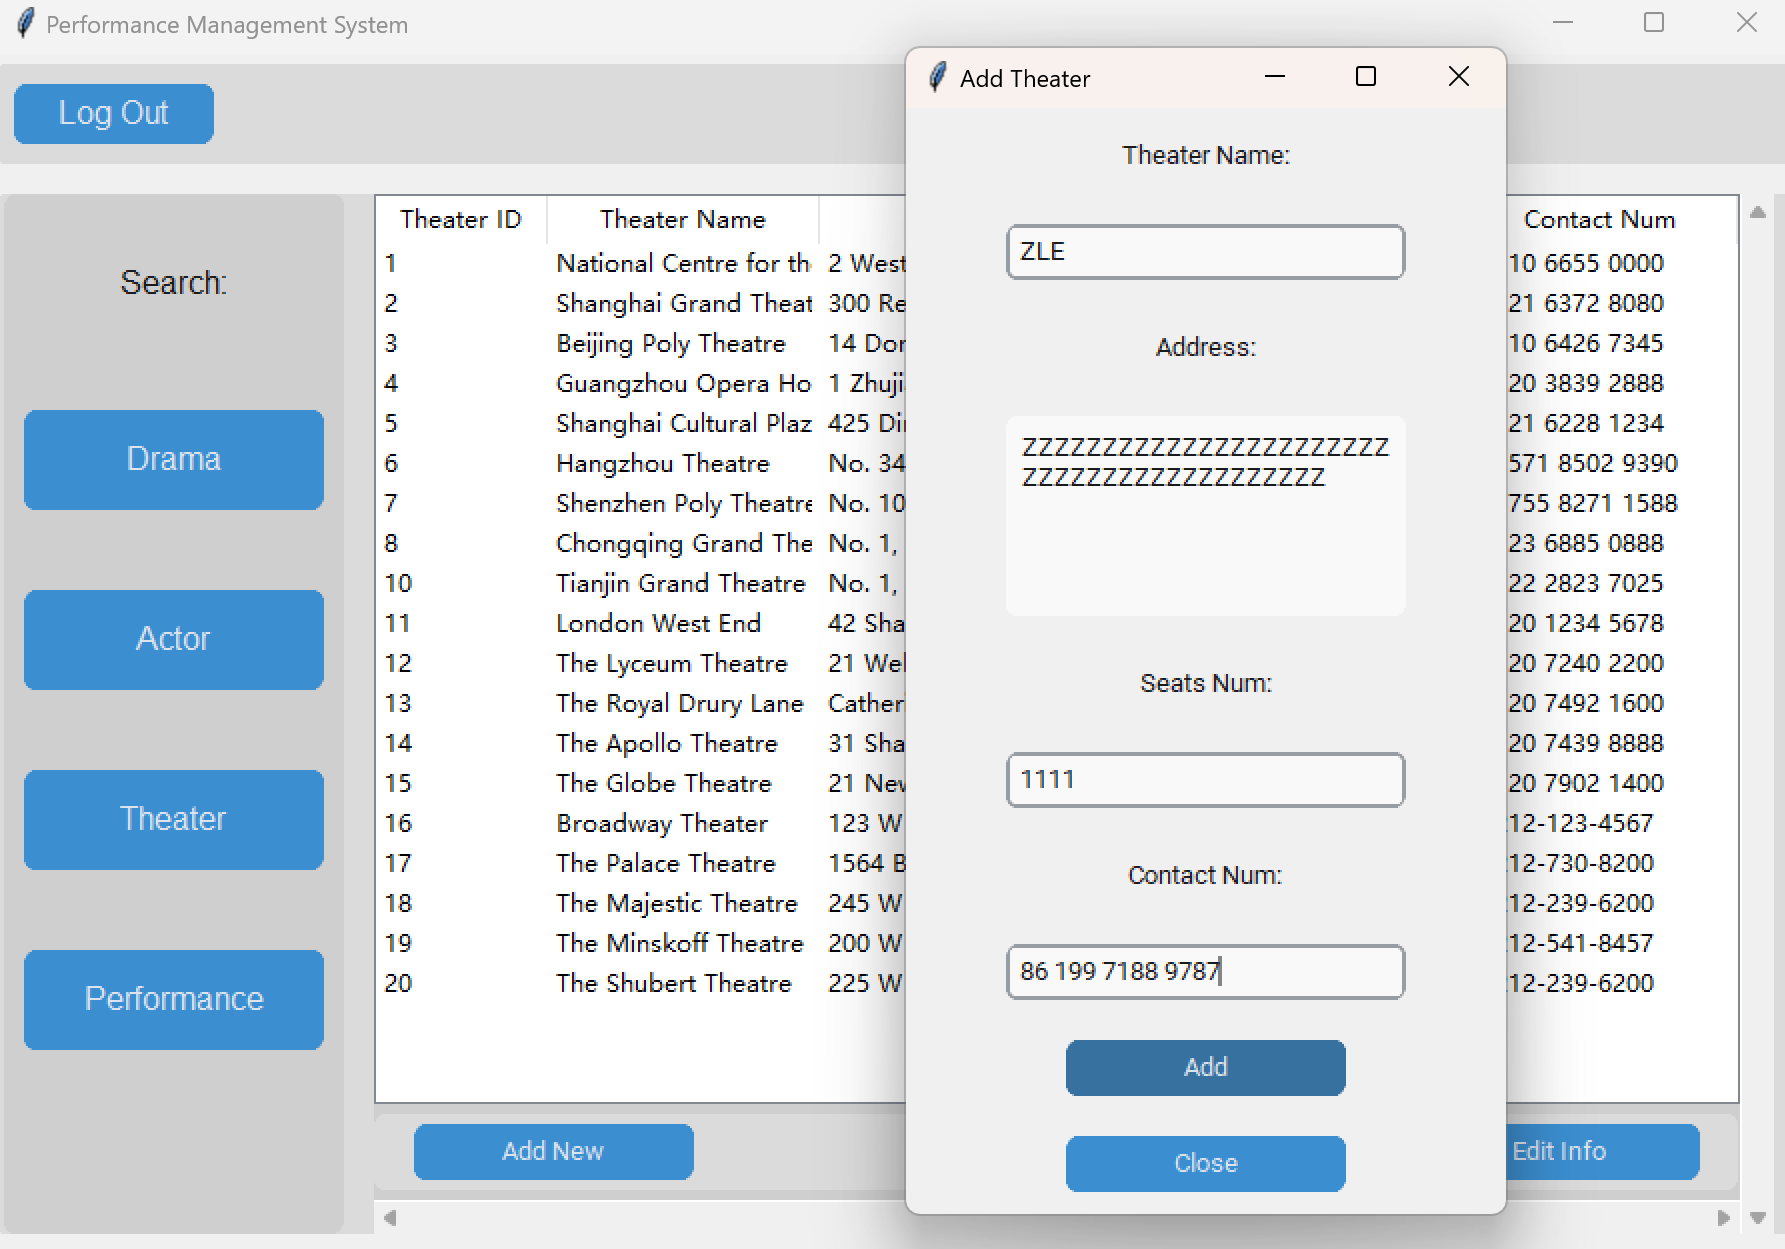
\includegraphics[width=\textwidth]{39.png}
        \caption{Theater add} 
        \label{Figure 39}
    \end{minipage}
    \hfill
    \begin{minipage}{0.48\textwidth}
        \centering
        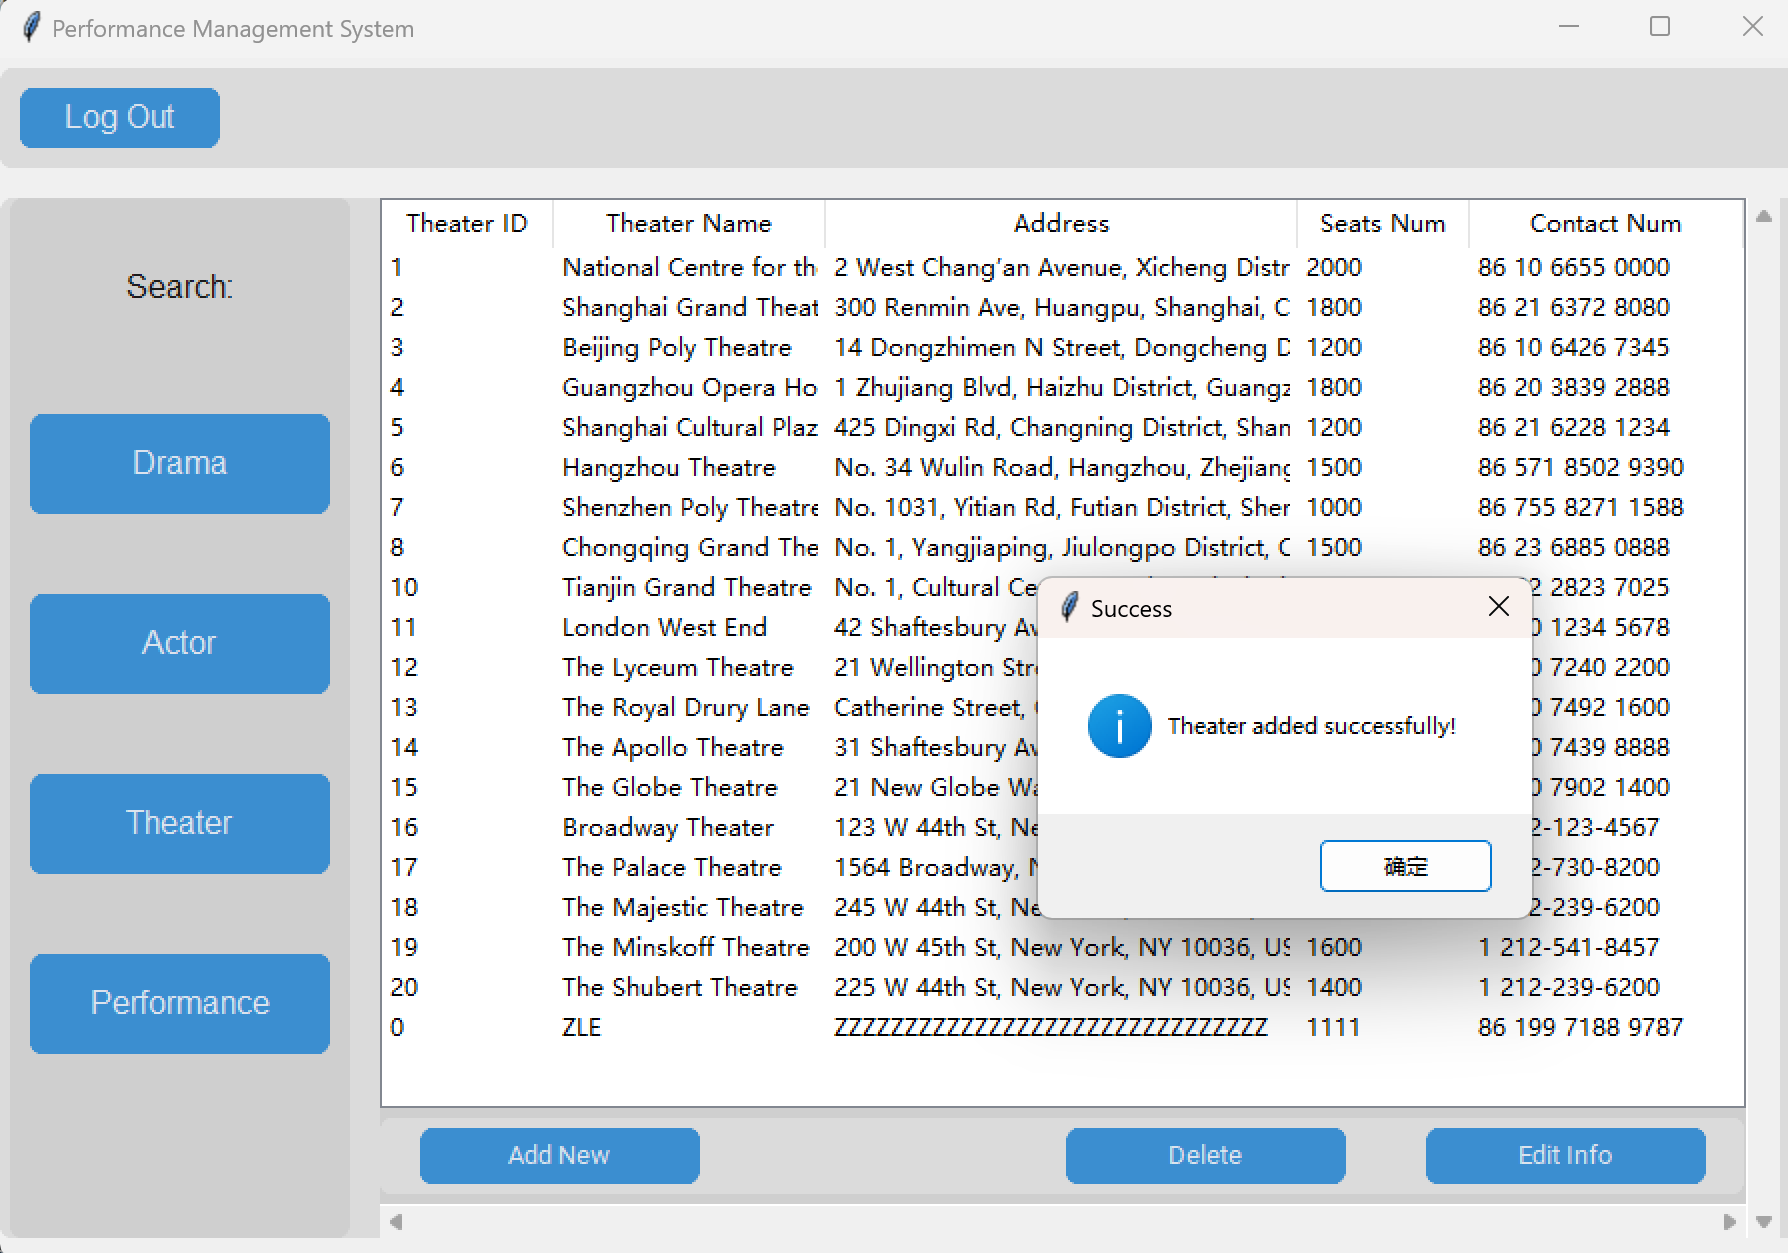
\includegraphics[width=\textwidth]{40.png}
        \caption{After add}
        \label{Figure 40}
    \end{minipage}
\end{figure}

\begin{figure}[H]
    \centering
    \begin{minipage}{0.48\textwidth}
        \centering
        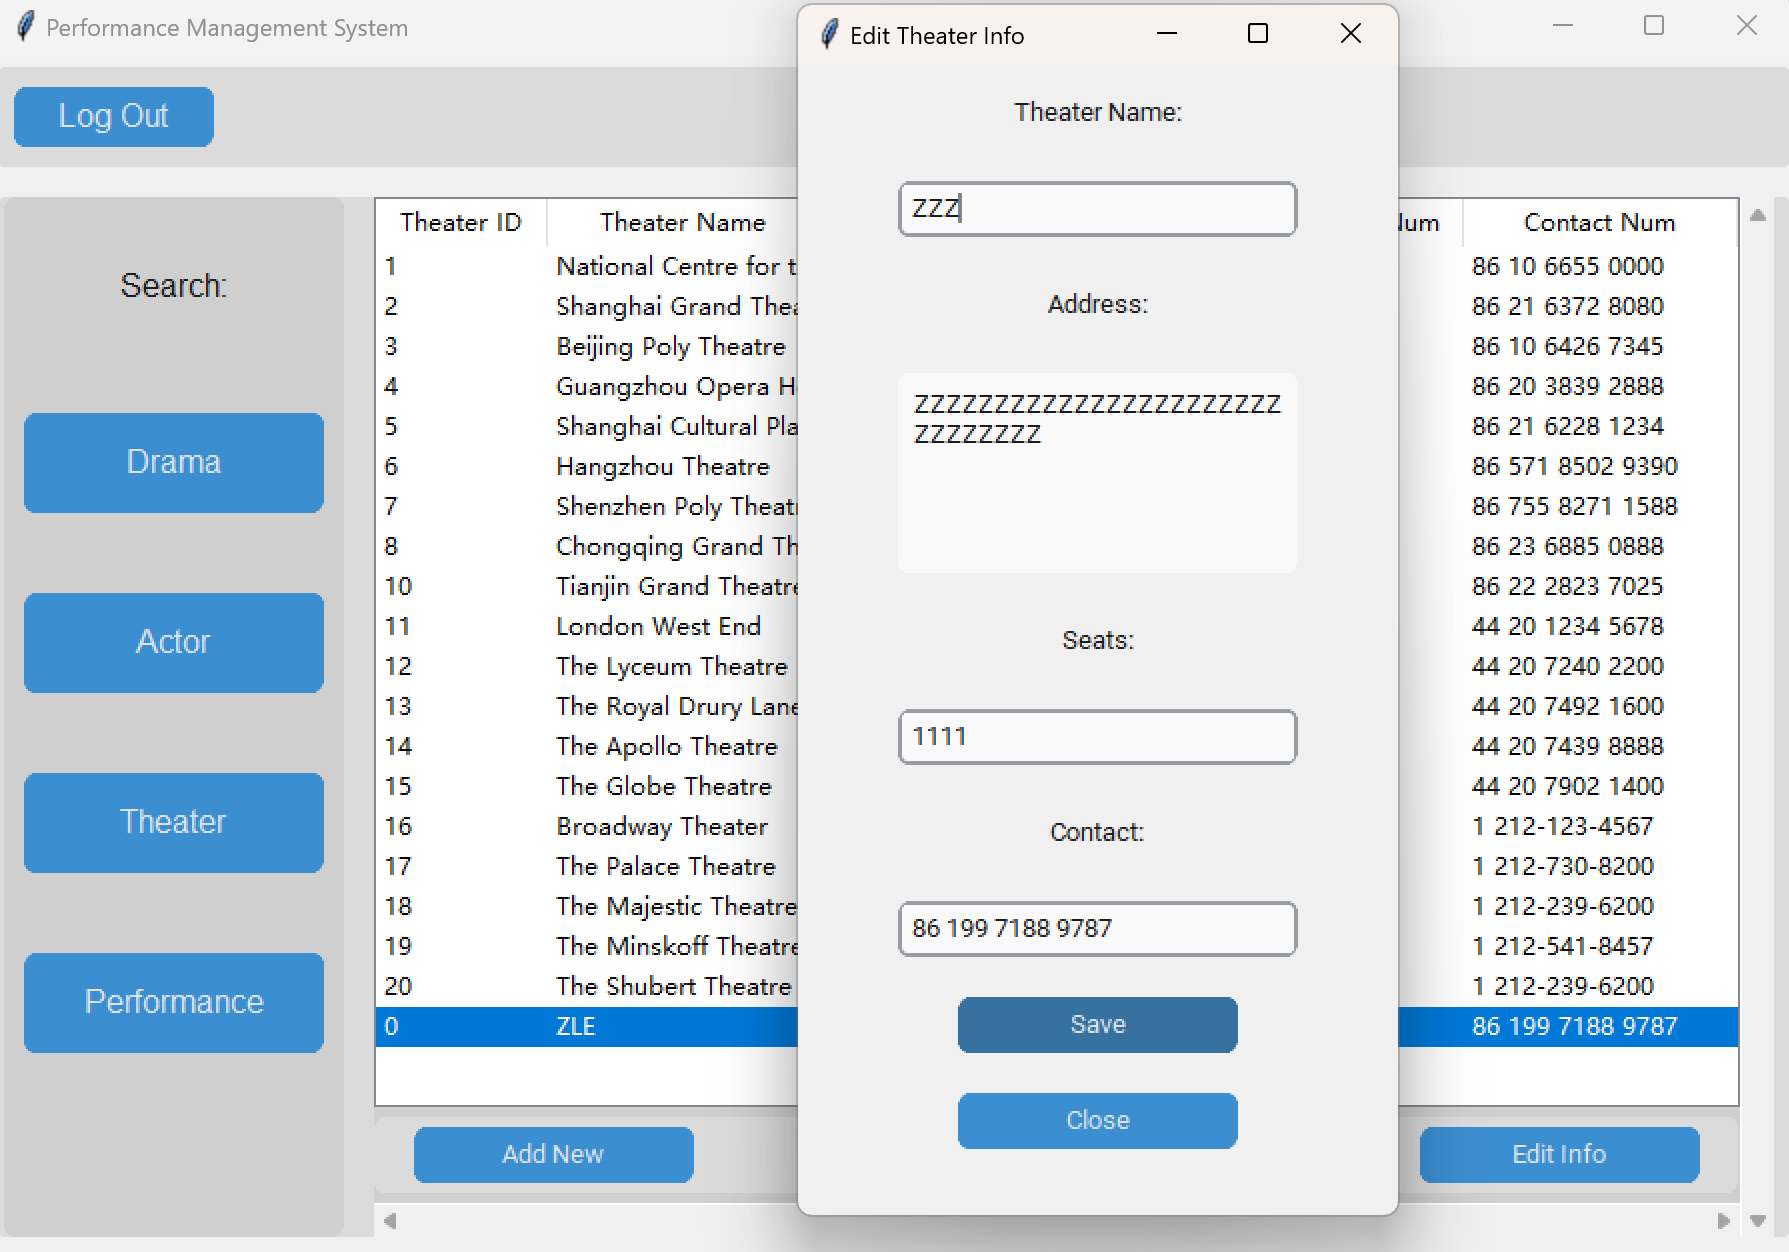
\includegraphics[width=\textwidth]{41.png}
        \caption{Theater edit} 
        \label{Figure 41}
    \end{minipage}
    \hfill
    \begin{minipage}{0.48\textwidth}
        \centering
        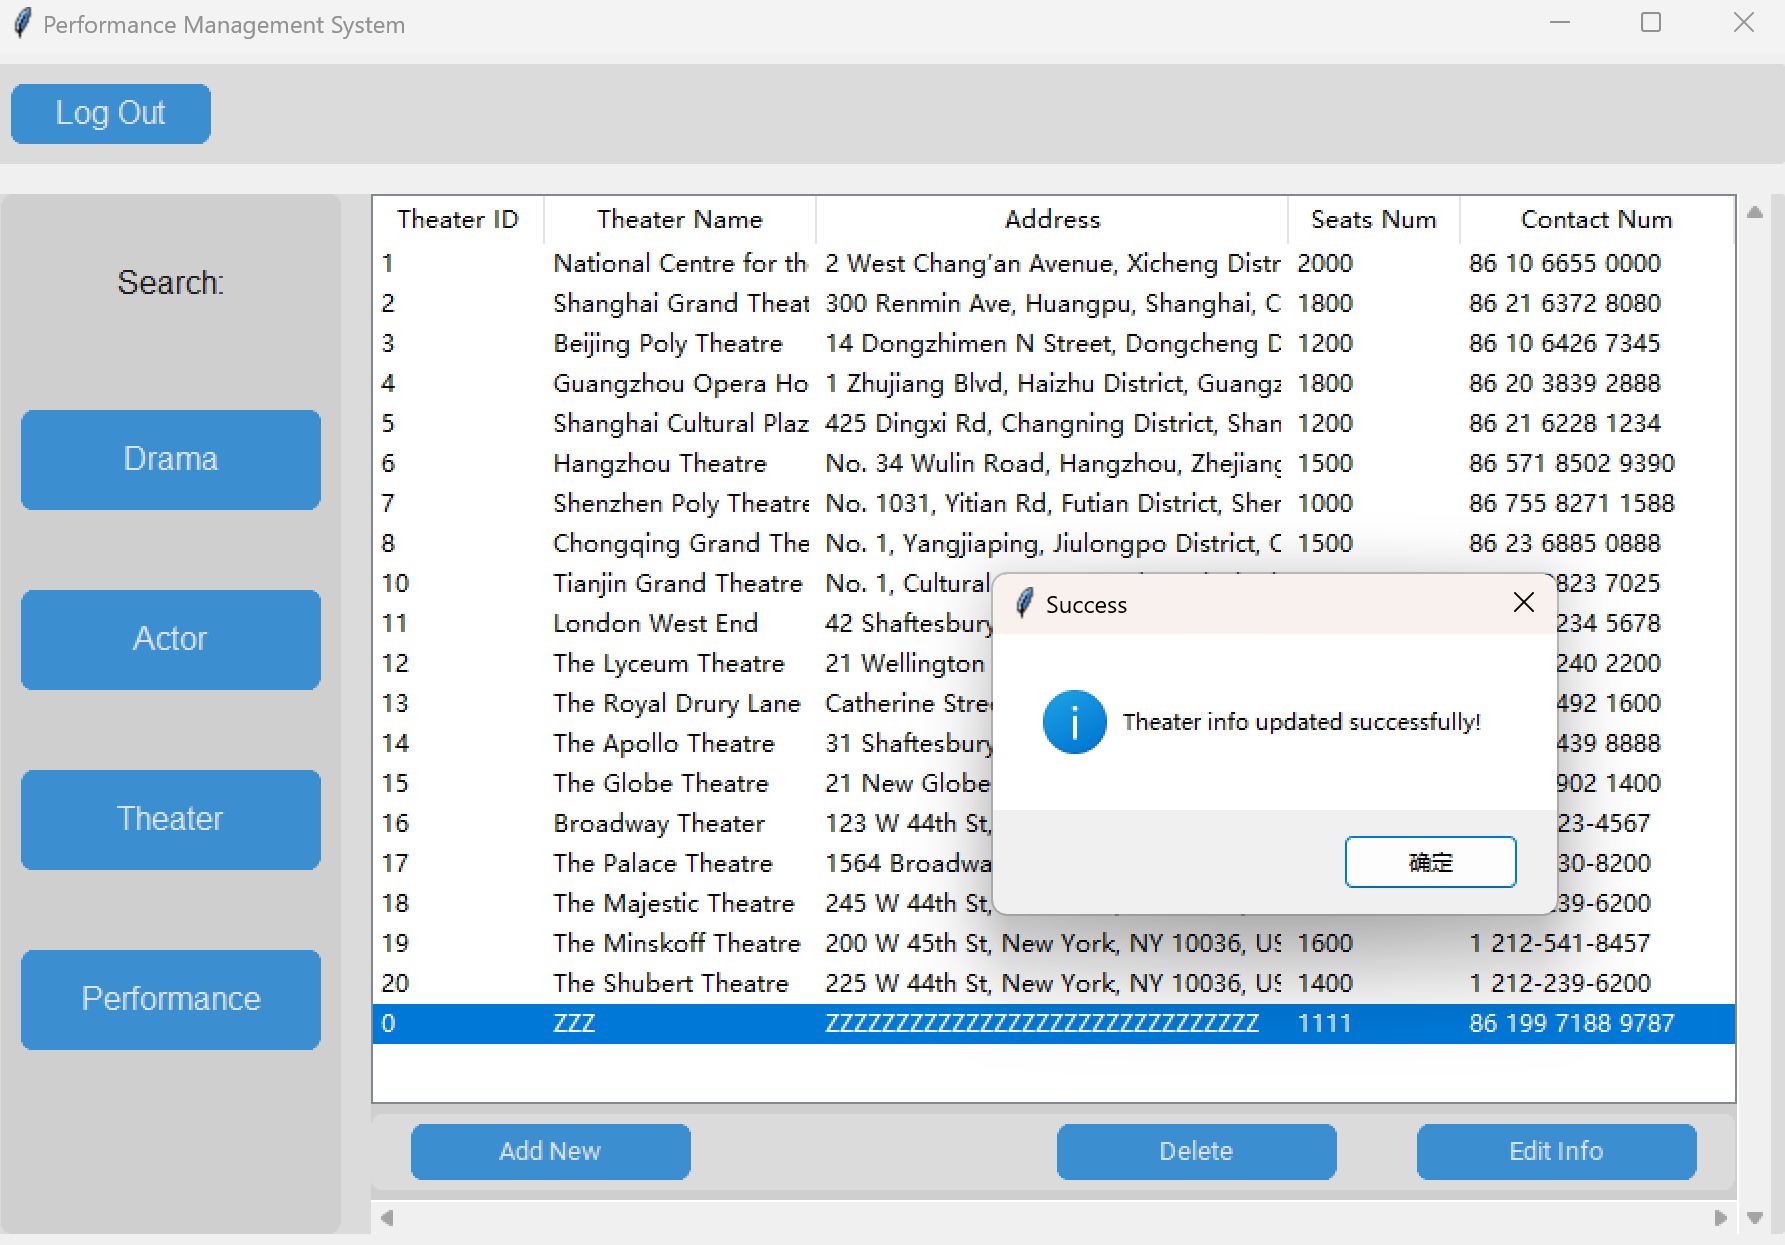
\includegraphics[width=\textwidth]{42.png}
        \caption{After edit}
        \label{Figure 42}
    \end{minipage}
\end{figure}

\subsubsection{Performance Management}
\par Clicking on 'Performance' displays all the performance information, with options to add, modify, or delete performance information and adjust charactors information using the corresponding buttons.\(Figure43-46\)

\begin{figure}[H]
    \centering
    \begin{minipage}{0.48\textwidth}
        \centering
        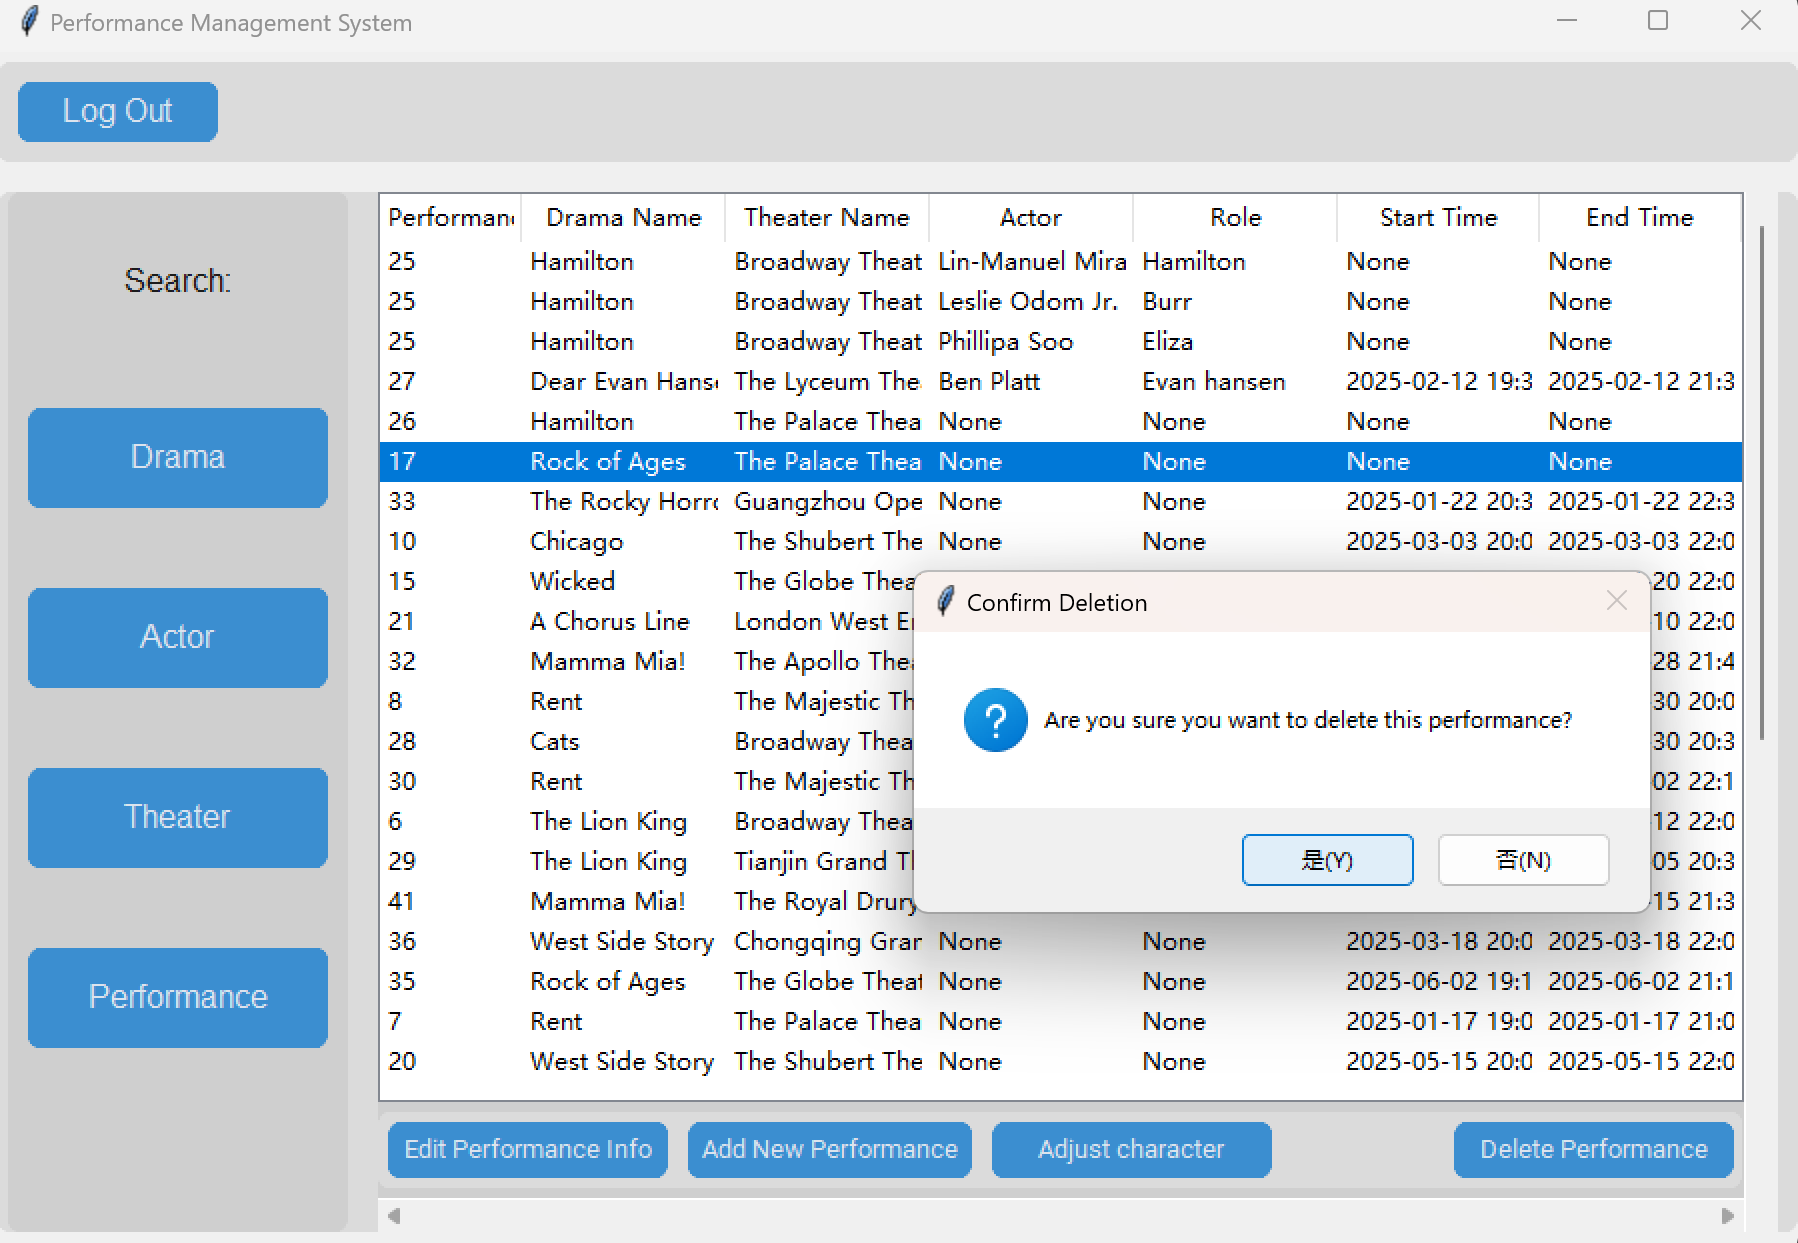
\includegraphics[width=\textwidth]{43.png}
        \caption{Performance delete} 
        \label{Figure 43}
    \end{minipage}
    \hfill
    \begin{minipage}{0.48\textwidth}
        \centering
        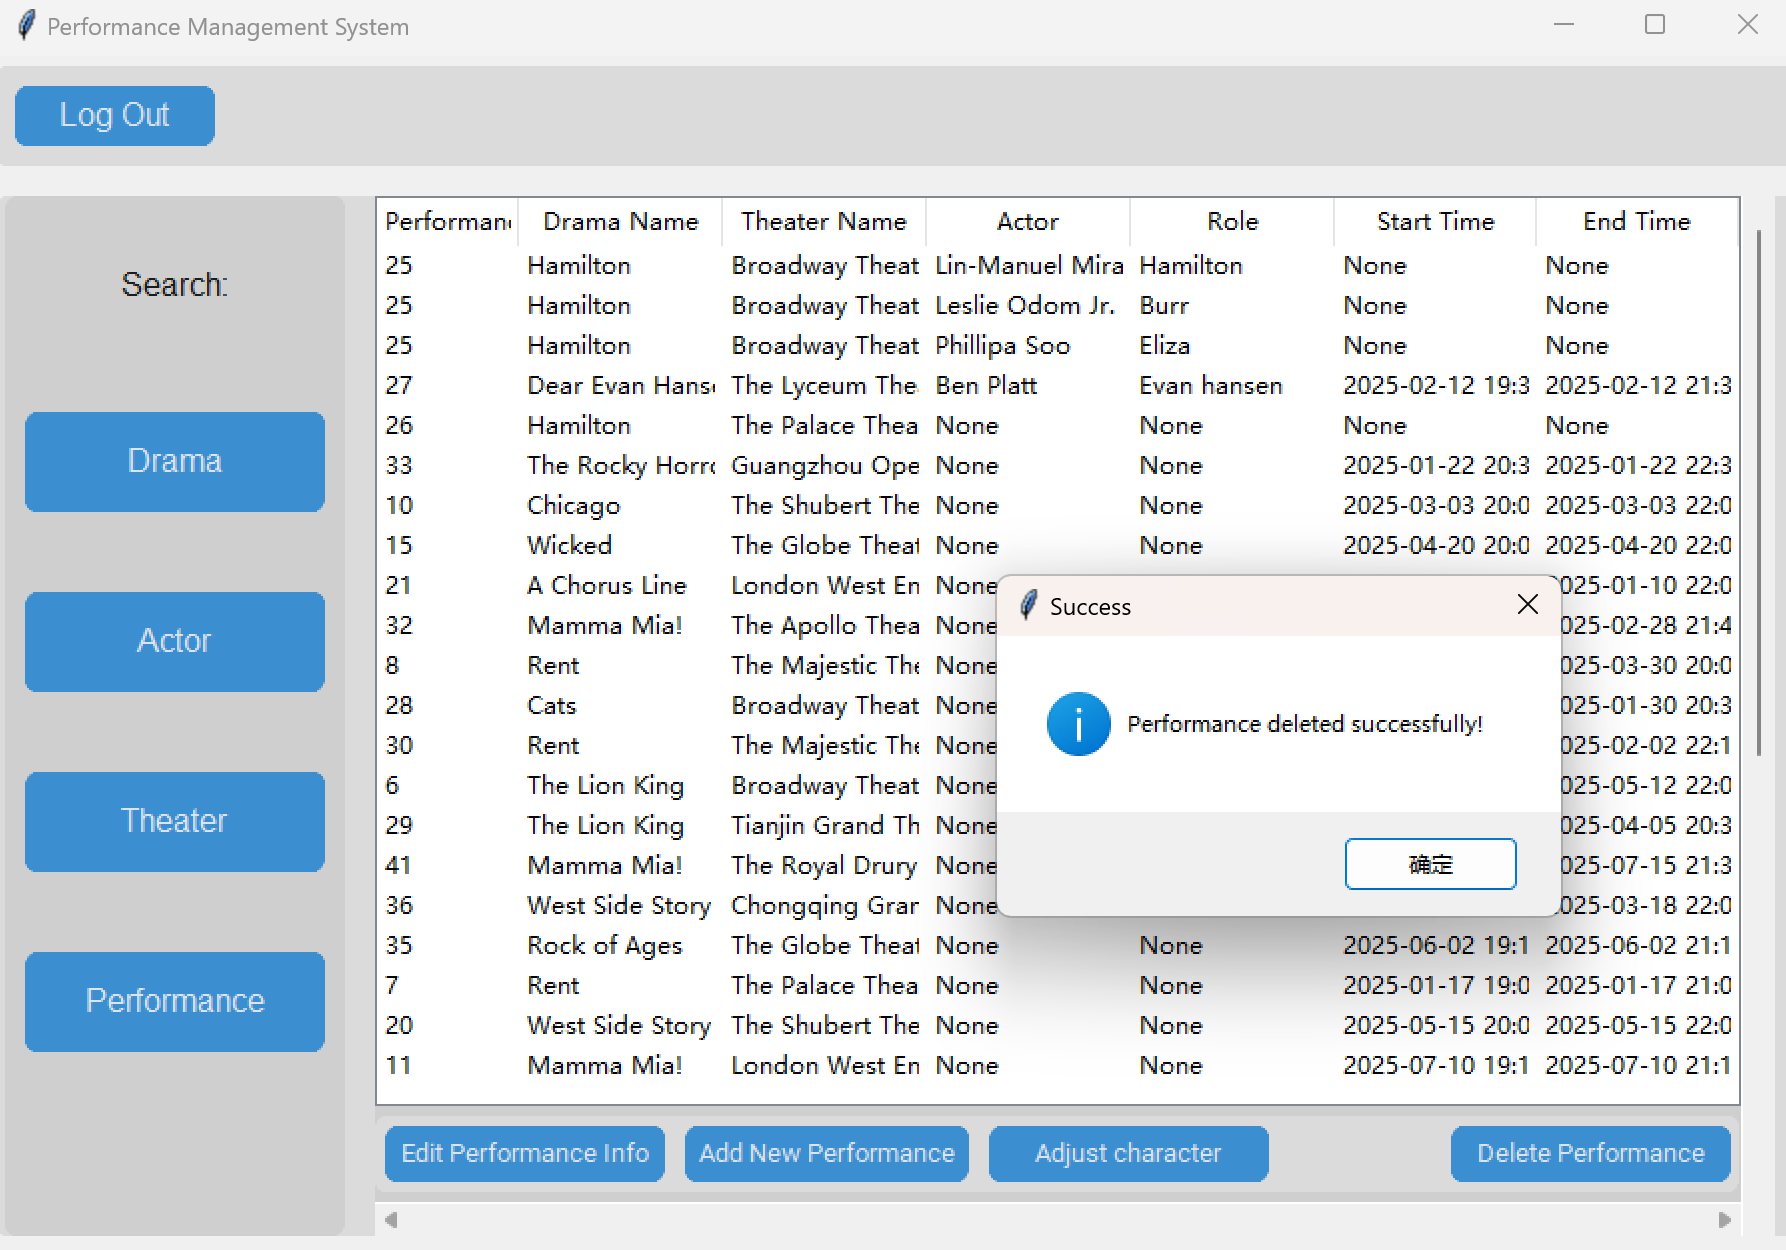
\includegraphics[width=\textwidth]{44.png}
        \caption{After deletion}
        \label{Figure 44}
    \end{minipage}
\end{figure}

\begin{figure}[H]
    \centering
    \begin{minipage}{0.48\textwidth}
        \centering
        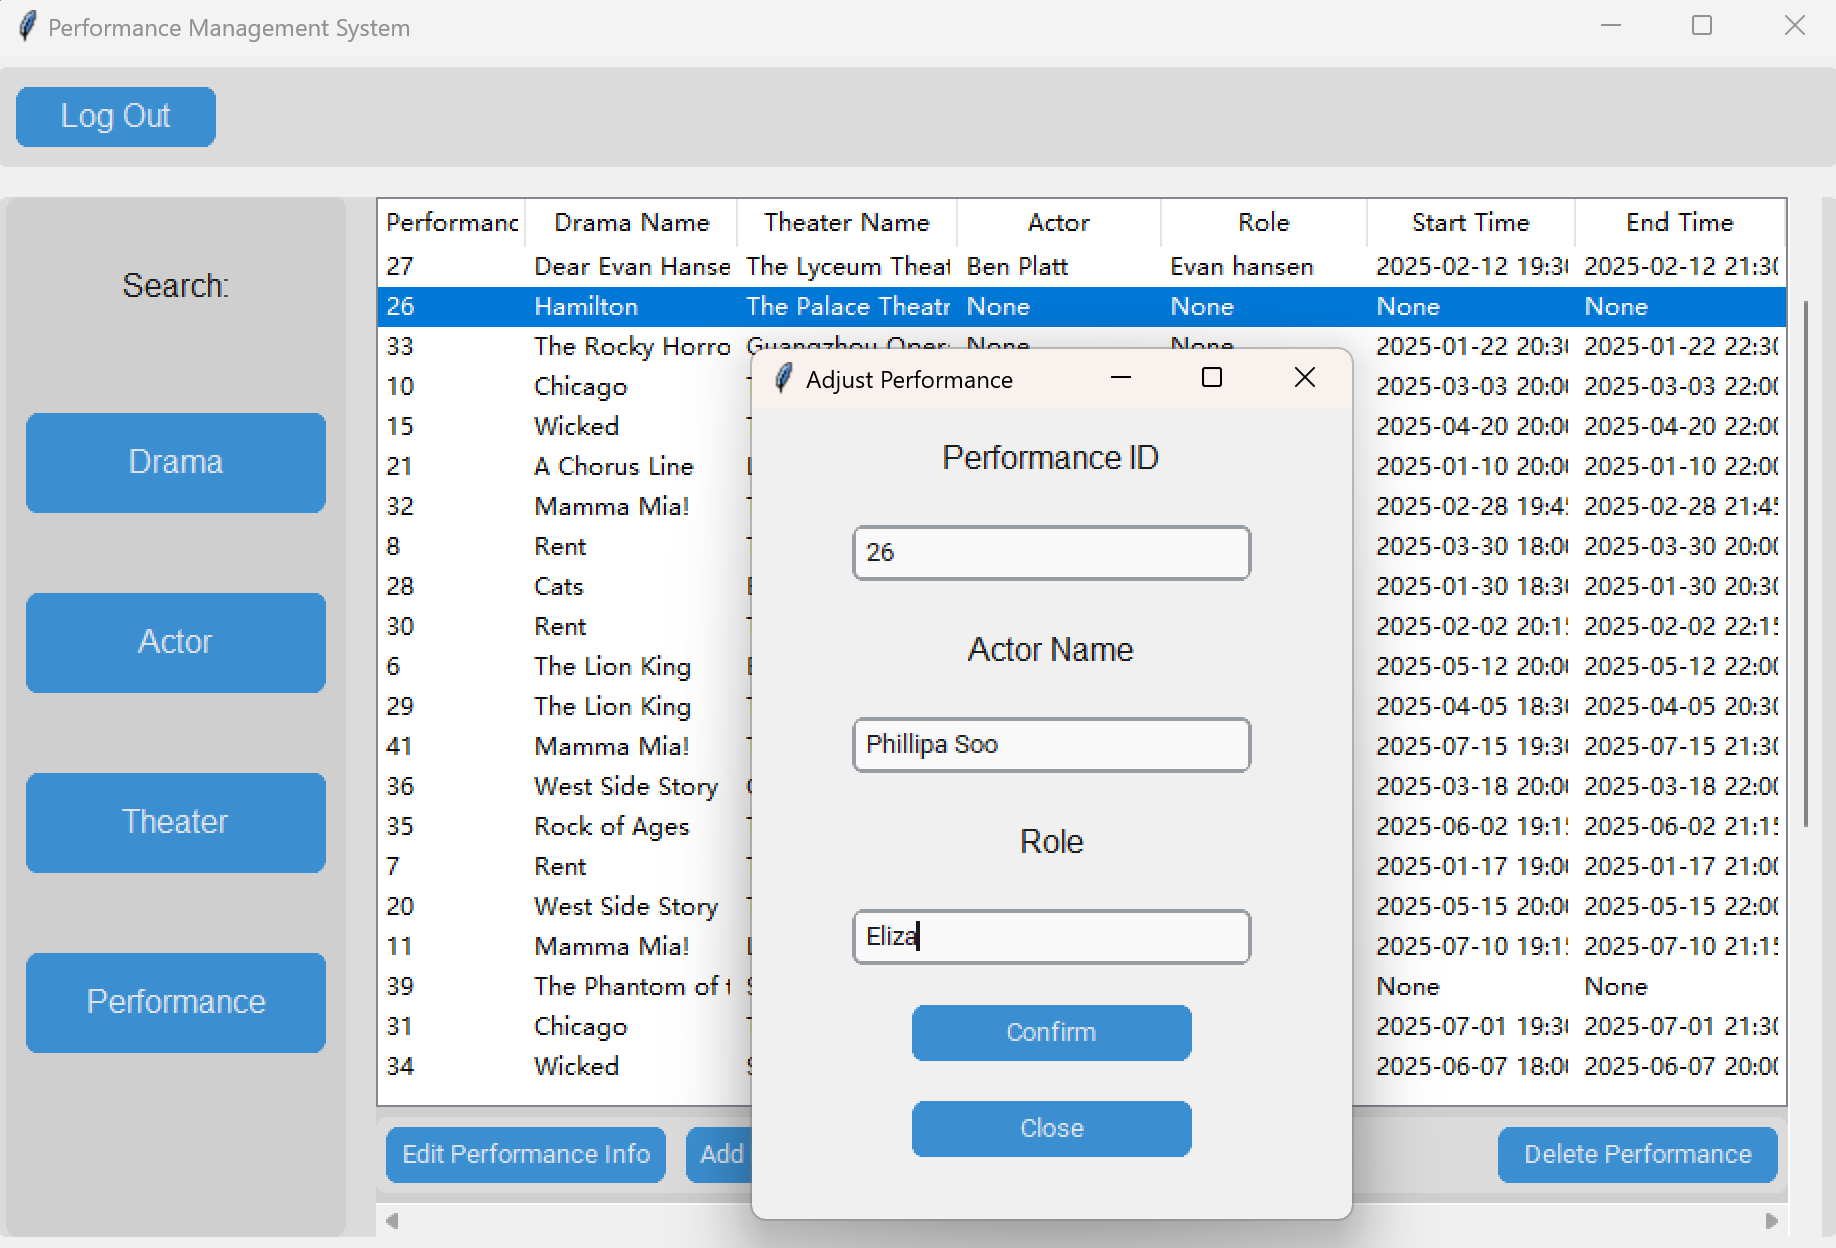
\includegraphics[width=\textwidth]{45.png}
        \caption{Charactor adjust} 
        \label{Figure 45}
    \end{minipage}
    \hfill
    \begin{minipage}{0.48\textwidth}
        \centering
        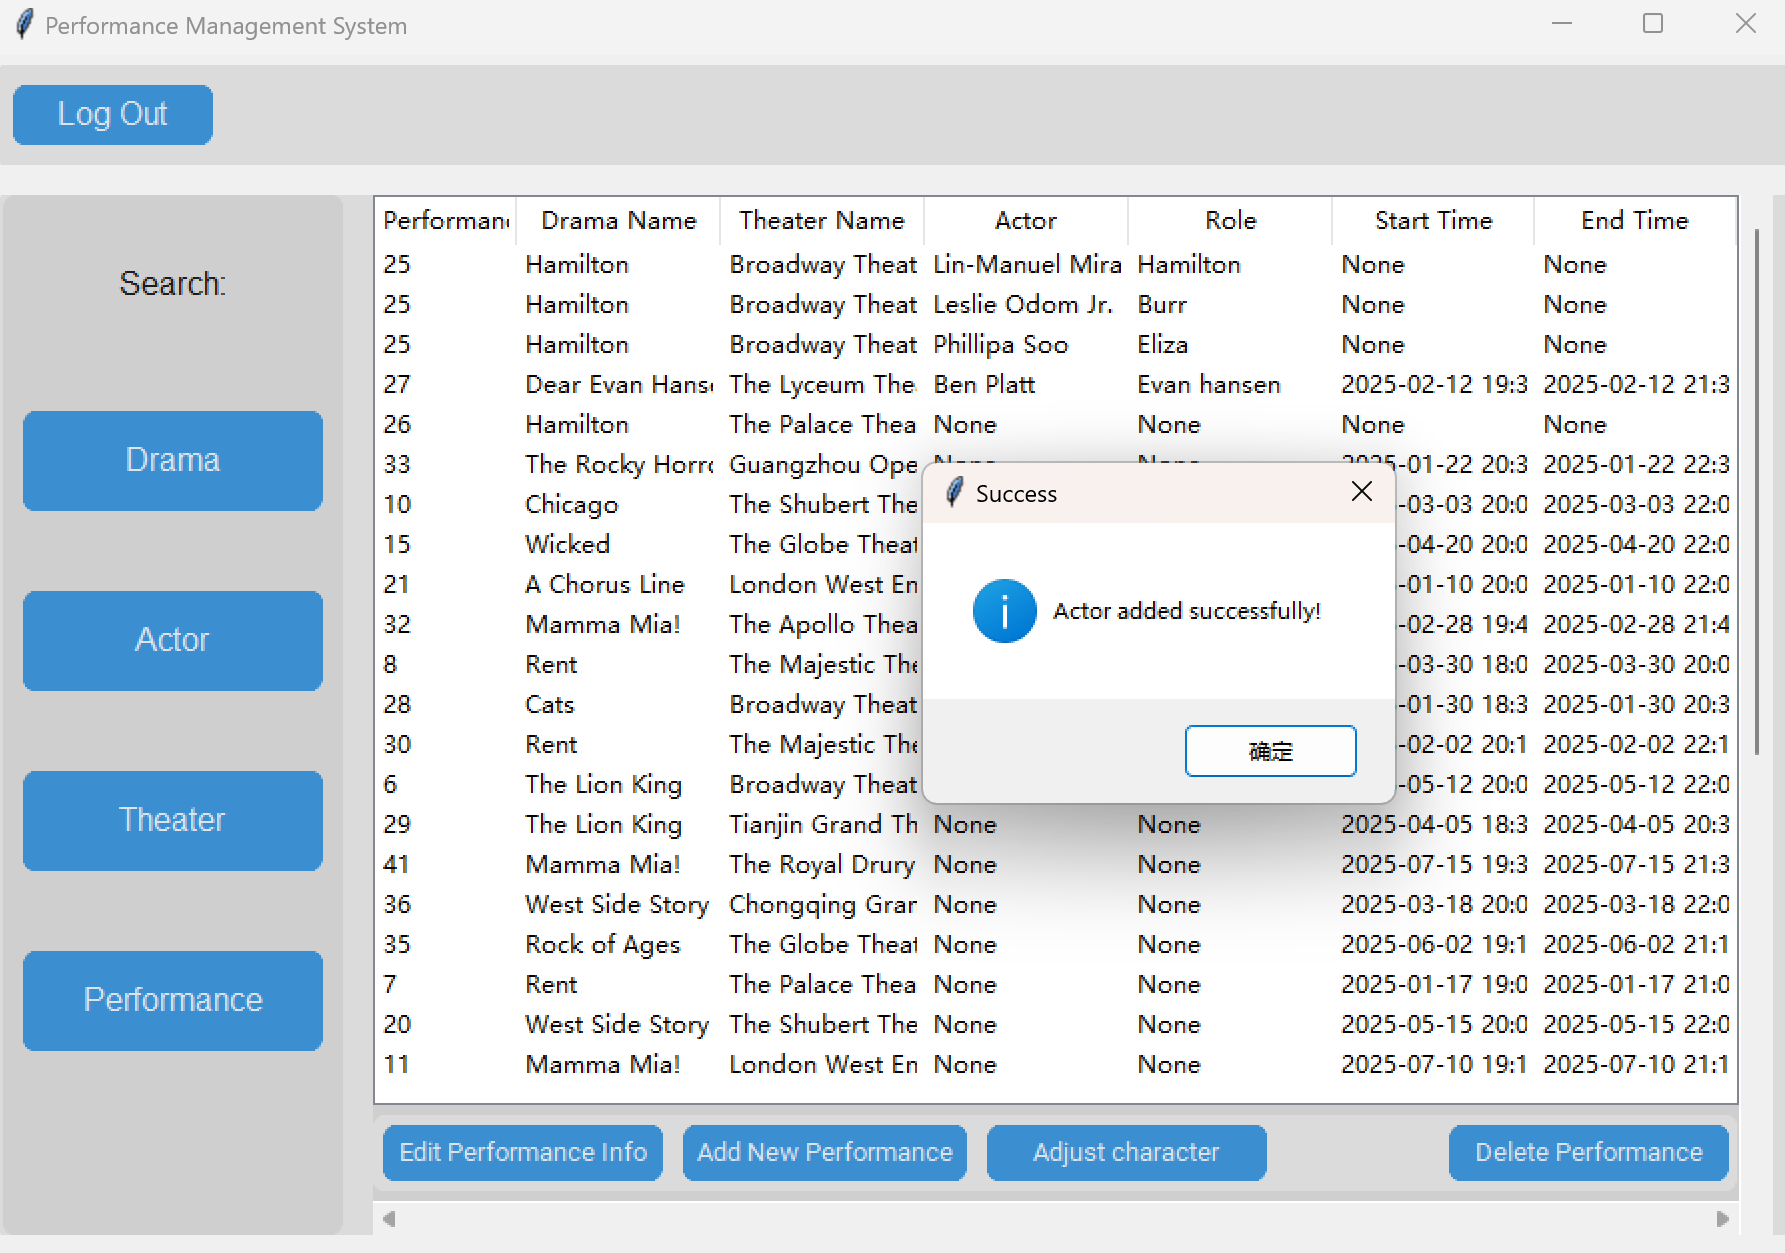
\includegraphics[width=\textwidth]{46.png}
        \caption{After adjust}
        \label{Figure 46}
    \end{minipage}
\end{figure}

\section{Conclusion}
\par Although a lot of effort has been put into this project, drawing inspiration from real-world performance systems and striving to improve functionality, time is limited, and there are still many areas that need refinement. For example, issues like the format for writing to the database, whether the performance schedule corresponds to the drama's duration, and certain constraints still need to be addressed. Additionally, some features are missing, such as allowing users to add comments, share and view comments, and enable ticket refunds. After the course, I will continue to study databases and further improve this program.

\end{document}
